\documentclass[acmtog,anonymous,review]{acmart}
% \documentclass[acmtog,review]{acmart}
% Replace with the assigned paper ID after completing the online form.
\acmSubmissionID{paper ID}

\usepackage{booktabs} % For formal tables

% TOG prefers author-name bib system with square brackets
\citestyle{acmauthoryear}
%\setcitestyle{nosort,square} % nosort to allow for manual chronological ordering



\usepackage[ruled]{algorithm2e} % For algorithms
\renewcommand{\algorithmcfname}{ALGORITHM}
\SetAlFnt{\small}
\SetAlCapFnt{\small}
\SetAlCapNameFnt{\small}
\SetAlCapHSkip{0pt}

% --- Float placement relief ------------------------------------------------
% [t]-only placement caused a large backlog of figures/tables/algorithms to
% queue past LaTeX's \topnumber / \totalnumber limits, dumping onto the
% final pages as a "float-only" block and producing trailing blank pages.
% Wide float-heavy sections (especially figure*) need enough placement
% freedom in ACM's two-column layout; otherwise LaTeX queues them and
% leaves sparse text pages while waiting for a legal top-of-page slot.
\usepackage{placeins} % provides \FloatBarrier; [section] option is
                      % forbidden by acmart (redefines \section).
\renewcommand{\topfraction}{0.95}
\renewcommand{\bottomfraction}{0.8}
\renewcommand{\textfraction}{0.05}
\renewcommand{\floatpagefraction}{0.6}
\renewcommand{\dbltopfraction}{0.95}
\renewcommand{\dblfloatpagefraction}{0.6}
\setcounter{topnumber}{4}
\setcounter{bottomnumber}{2}
\setcounter{totalnumber}{6}
\setcounter{dbltopnumber}{3}
\setlength{\floatsep}{6pt plus 2pt minus 2pt}
\setlength{\textfloatsep}{8pt plus 2pt minus 2pt}
\setlength{\dblfloatsep}{6pt plus 2pt minus 2pt}
\setlength{\dbltextfloatsep}{8pt plus 2pt minus 2pt}

% --- Tagged equation environment (fix hyperref duplicate destinations) -----
% amsmath's \tag{...} replaces the visible equation number but rolls the
% equation counter back at \end{equation}, so multiple \tag-labelled
% equations all end up placing their hyperref anchor at the SAME
% counter value (e.g. equation.24), triggering pdfTeX's "destination
% with the same identifier has been already used, duplicate ignored"
% warnings and breaking \ref navigation to the later tagged eqs.
%
% Workaround: use equation* (unnumbered, no counter anchor) and manually
% set \@currentlabel so \ref prints the custom tag. \phantomsection
% creates a unique hyperref destination right before the equation so
% each \label binds to its own fresh anchor. Usage:
%     \begin{taggedeqn}{P}{P}
%         \hat{\boldsymbol{\theta}} = \arg\min ...
%     \end{taggedeqn}
% First arg is the visible tag text, second is the slug for eq:<slug>.
\makeatletter
\newenvironment{taggedeqn}[2]{%
    \gdef\@currentlabel{#1}%
    \phantomsection\label{eq:#2}%
    \begin{equation*}\tag*{(#1)}%
}{%
    \end{equation*}%
}
\makeatother

% --- Typography relief -----------------------------------------------------
% Let TeX stretch inter-word spacing by up to 3em on tight paragraphs before
% declaring an overfull hbox. This absorbs most small-to-medium overflows
% from long inline math, \texttt{long/file/paths.py}, and multi-line
% compound adjectives without manual line-break hints. Tune down if the
% inter-word spacing becomes visually uneven.
\emergencystretch=3em
\hbadness=2000   % mute "Underfull \hbox" complaints below this badness
\hfuzz=1pt       % tolerate up to 1pt overfull without reporting

% --- Figure placeholder mode ---------------------------------------------
% When \figplaceholdertrue is set, draft-only figures render as framed
% placeholder boxes. The normal submission path is \figplaceholderfalse:
% \figureorplaceholder / \widefigureorplaceholder render the image when
% the file exists and fall back to the same box only when the file is
% still absent.
\newif\iffigplaceholder
\figplaceholderfalse

\newcommand{\figplaceholder}[2][6cm]{%
    \fbox{\parbox[c][#1][c]{0.94\columnwidth}{%
        \centering\small\itshape #2}}%
}
\newcommand{\figplaceholderwide}[2][6cm]{%
    \fbox{\parbox[c][#1][c]{0.97\textwidth}{%
        \centering\small\itshape #2}}%
}
\newcommand{\figureorplaceholder}[4][6cm]{%
    \iffigplaceholder
        \figplaceholder[#1]{#4}%
    \else
        \IfFileExists{#3}{\includegraphics[width=#2]{#3}}{%
            \figplaceholder[#1]{#4}}%
    \fi
}
\newcommand{\widefigureorplaceholder}[4][6cm]{%
    \iffigplaceholder
        \figplaceholderwide[#1]{#4}%
    \else
        \IfFileExists{#3}{\includegraphics[width=#2]{#3}}{%
            \figplaceholderwide[#1]{#4}}%
    \fi
}

% Metadata Information
\acmJournal{TOG}
%\acmVolume{38}
%\acmNumber{4}
%\acmArticle{39}
%\acmYear{2019}
%\acmMonth{7}

% Copyright
%\setcopyright{acmcopyright}
%\setcopyright{acmlicensed}
%\setcopyright{rightsretained}
%\setcopyright{usgov}
%\setcopyright{usgovmixed}
%\setcopyright{cagov}
%\setcopyright{cagovmixed}

% DOI
%\acmDOI{0000001.0000001_2}

% Paper history
%\received{February 2007}
%\received{March 2009}
%\received[final version]{June 2009}
%\received[accepted]{July 2009}


% Document starts
\begin{document}
% Title portion
\title{Fast Non-Newtonian ViRheometry via Local Gaussian-Process Surrogates}

% Authors (suppressed automatically by acmart [anonymous] flag during
% review; will render in the camera-ready when the [anonymous] option
% is removed from \documentclass).
\author{Yuxiang Xiong}
\email{billxiong021@gmail.com}
\affiliation{%
  \institution{Aoyama Gakuin University (AGU)}
  \country{Japan}
}
\author{Mitsuki Hamamichi}
\email{hammik.1231@gmail.com}
\affiliation{%
  \institution{Aoyama Gakuin University (AGU)}
  \country{Japan}
}
\author{Yonghao Yue}
\email{yonghao@it.aoyama.ac.jp}
\affiliation{%
  \institution{Aoyama Gakuin University (AGU)}
  \streetaddress{O-525, Fuchinobe 5-10-1, Chuo-ku}
  \city{Sagamihara}
  \state{Kanagawa}
  \postcode{252-5258}
  \country{Japan}
}

\renewcommand\shortauthors{Xiong, Y. et al.}

\begin{abstract}
We estimate Herschel--Bulkley (HB) parameters $(n,\eta,\sigma_Y)$
from calibrated dam-break observations using a fixed local
Gaussian-process (GP) surrogate. A bank of $2{,}775$ experts is constructed from a cleaned
$407{,}480$-row simulation corpus, with GP fitting restricted to
$325{,}984$ training rows; $2{,}735$ experts are eligible for inverse use. It predicts eight signed front displacements
from material parameters and setup geometry. Within compatible local
supports, bounded continuous CMA-ES jointly fits one material triple
using a Gaussian marginal objective with GP/BAE and observation-error
allowances. The output includes applicability and raw-fit status;
online inversion calls no physical simulator.

Assigned-expert evaluation on $40{,}748$ test rows gives MAE
$0.05297$\,cm, conditional on the response-informed partition.
In a synthetic perturbation study, 62 of 64 fits on 40 parameter
truths pass the raw-fit gate, while substantial parameter and curve
errors remain. On six rheometer-reference materials, mean joint
flow-curve discrepancy is $0.271667$ in natural-log stress RMS.
Recorded joint fits take $13.058$--$25.241$\,s for these materials
and $5.192$--$25.409$\,s for a separate freshness collection, excluding
acquisition, preprocessing and offline replay.

The freshness comparison predicts the same original-batch third
observation from same-batch fast inputs or a simulation-based workflow
using a later remade-batch second capture. Mean IoU over six materials
and 48 frames is $0.913819$ versus $0.877112$. The comparison supports
shorter computational waiting as a practical measurement goal, without
isolating material-change effects. Proxy fit, physical curve agreement,
cross-setup prediction and parameter uniqueness remain distinct claims.

\end{abstract}


%
% The code below should be generated by the tool at
% http://dl.acm.org/ccs.cfm
% Please copy and paste the code instead of the example below.
%

\begin{CCSXML}
<ccs2012>
 <concept>
  <concept_id>10010147.10010371.10010396.10010398</concept_id>
  <concept_desc>Computing methodologies~Physical simulation</concept_desc>
  <concept_significance>500</concept_significance>
 </concept>
 <concept>
  <concept_id>10010147.10010257.10010293</concept_id>
  <concept_desc>Computing methodologies~Computer graphics</concept_desc>
  <concept_significance>300</concept_significance>
 </concept>
 <concept>
  <concept_id>10010147.10010178.10010224</concept_id>
  <concept_desc>Computing methodologies~Machine learning</concept_desc>
  <concept_significance>300</concept_significance>
 </concept>
</ccs2012>
\end{CCSXML}


% \begin{CCSXML}
% <ccs2012>
%  <concept>
%   <concept_id>10010520.10010553.10010562</concept_id>
%   <concept_desc>Computer systems organization~Embedded systems</concept_desc>
%   <concept_significance>500</concept_significance>
%  </concept>
%  <concept>
%   <concept_id>10010520.10010575.10010755</concept_id>
%   <concept_desc>Computer systems organization~Redundancy</concept_desc>
%   <concept_significance>300</concept_significance>
%  </concept>
%  <concept>
%   <concept_id>10010520.10010553.10010554</concept_id>
%   <concept_desc>Computer systems organization~Robotics</concept_desc>
%   <concept_significance>100</concept_significance>
%  </concept>
%  <concept>
%   <concept_id>10003033.10003083.10003095</concept_id>
%   <concept_desc>Networks~Network reliability</concept_desc>
%   <concept_significance>100</concept_significance>
%  </concept>
% </ccs2012>
% \end{CCSXML}

\ccsdesc[500]{Computing methodologies~Physical simulation}
\ccsdesc[300]{Computing methodologies~Computer graphics}
\ccsdesc[300]{Computing methodologies~Machine learning}

%
% End generated code
%


\keywords{Material parameter estimation, Herschel--Bulkley,
non-Newtonian fluids, video-based estimation, Gaussian-process
surrogates, continuous numerical inversion, Bayesian approximation
error, multi-setup measurement}


% Teaser omitted in this draft to avoid duplicating the method overview.

\maketitle

\section{Introduction}

Many everyday fluids---yogurts, pastes, sauces, slurries, cosmetic
emulsions---exhibit non-Newtonian behaviour that governs how they
pour, spread, cling, and deform. Parallel-plate and cone-and-plate
rheometers measure this behaviour through a controlled-gap shear
flow, but fail on materials with inclusions larger than the
measurement gap and on materials whose rheology evolves faster than
the lab procedure can capture.

Non-Newtonian video rheometry~\cite{hamamichi2023nonnewtonian}
addresses this gap by estimating Herschel--Bulkley parameters
from a simple dam-break flow: a material point
method (MPM) forward model is repeatedly executed inside an optimiser
until the simulated flow reproduces the observed silhouette. The
approach handles materials that instrumental rheometers cannot, but its
inner loop takes \emph{around eight hours per experimental setup}. This
latency is especially limiting for materials whose state changes during
measurement---sedimentation, ageing, temperature drift, mixing history,
or cooking cooldown---because the recovered parameter may describe a
past state rather than the current batch. Our goal is therefore not to
change the dam-break physics model, but to make the same forward
relation cheap enough for interactive inverse queries, ambiguity
diagnostics, and repeated freshness checks.

We use a fixed local GP bank to evaluate a continuous inverse objective.
Once calibrated observations are available, bounded CMA-ES jointly fits
one HB parameter triple to the measured setups. The recorded joint fits
take $13.058$--$25.241$\,s for six rheometer-reference materials and
$5.192$--$25.409$\,s for a separate freshness collection. These intervals
include expert selection, numerical search and fit assessment, with
initial forward construction, acquisition, preprocessing and offline
physical replay excluded. We evaluate forward approximation, synthetic
recovery, external flow curves, cross-setup image prediction and cost
as separate questions. Both the simulation-based baseline and our method
use CMA-ES; the computational change replaces repeated physical-forward
calls with fixed-surrogate evaluations.

\emph{(i) Local Gaussian-process (GP) forward surrogate.}
We replace repeated MPM calls by a pre-trained bank of local
Gaussian-process models. The surrogate maps
$(n,\eta,\sigma_Y,W,H)$ to the eight dam-break flow-front positions
$(x_{01},\ldots,x_{08})$ and provides both a prediction and an
uncertainty estimate for inverse estimation. The eight outputs are used
directly; we do not compress them with principal component analysis
(PCA).

\emph{(ii) Supported continuous inversion and quality reporting.}
We select compatible local expert supports and minimise a Gaussian
marginal objective using GP/BAE and observation-error allowances.
The solver returns an HB point estimate with applicability and per-setup
raw-fit status, or an explicit failure. A passing trajectory fit does
not certify parameter uniqueness, physical accuracy or calibrated
confidence. Synthetic recovery and external validation test those
distinct limitations rather than treating a low surrogate loss as truth.

\emph{(iii) Freshness-oriented sequential-measurement evaluation.}
We evaluate two observations acquired close together from one preparation
against a third observation from that preparation. We also complete a
simulation-based workflow that reuses the same first observation but
acquires its recommended second observation from a later, remade batch.
Both frozen estimates predict the same original third observation.
This compares the predictive behaviour and computational burden of the
two workflows; it does not isolate material change from geometry,
observation or numerical effects, or fit a kinetic ageing law.

Hamamichi et al.~\cite{hamamichi2023nonnewtonian} established
the dam-break observation and multi-setup formulation used here.
We retain their physical motivation and optional setup criterion,
while accelerating the forward evaluations used by numerical inversion.
The real-material results use fixed measured geometries. The proposal
module is assessed separately and is not credited with selecting those
geometries or proving that additional observations always improve recovery.

\section{Related Work}

\subsection{Physical Measurements and Flow Rheology Signals}

Quantitative rheology is traditionally measured with rheometers
(parallel-plate, cone-and-plate, or rotational) that apply a
controlled laminar flow under known shear rate to recover the
constitutive relation between shear stress and shear rate. These
instruments require a narrow gap to enforce a clean shear profile,
which excludes materials with millimeter-scale inclusions, as well
as materials whose rheology evolves faster than the lab procedure
can capture. Less-controlled but more accessible alternatives, such
as the Bostwick consistometer, give a single readable measurement
from a simple dam-break test.

Gravity-driven flow has a long pedigree as a rheometric observation
that complements idealized-flow rheometers. The slump test
of~\citet{pashias1996fifty} recovers yield stress from a single
geometric reading; \citet{roussel2005fiftycent} extend this argument
to the spreading regime that matches dam-break geometry directly;
the final-deposit shape of a stopped free-surface flow is itself a
rheological signature~\cite{coussot1996rheological};
and~\citet{ancey2007plasticity} frames the broader class of
gravity-driven yield-stress flows as a standard rheometric regime.
The relation between flow-front position and Herschel--Bulkley
parameters is made quantitative by the similarity analyses
of~\citet{liumei1989slow} and~\citet{balmforth2007two}, the same
analytic framework used by~\citet{hamamichi2023nonnewtonian} to
explain when different Herschel--Bulkley triples produce similar
dam-break trajectories.

Our forward simulator inherits the MPM lineage brought into
graphics by~\cite{stomakhin2013material,jiang2015affine,hu2018moving,
jiang2016material}, with yield-stress rheology realised through
return-mapping
formulations~\cite{yue2015continuum,ram2015material,klar2016drucker,
tampubolon2017multi,wolper2019cdmpm}. We use the Herschel--Bulkley
return map of~\citet{yue2015continuum} on
Taichi~\cite{hu2019taichi}; \citet{nagasawa2019mixing}, from the
same lab as our predecessor, shares our material focus.


\subsection{Video-Based Material Estimation}

Estimating simulation parameters from video by matching rendered and
observed dynamics has a long lineage in graphics and
vision~\cite{bhat2002computing,monszpart2016smash}.
\citet{takahashi2019video} established the video-to-parameter pattern
for viscous fluids by matching rendered and observed dam-break
silhouettes per scene; \citet{hamamichi2023nonnewtonian} extended
this to the Herschel--Bulkley triple $(n,\eta,\sigma_Y)$ and is the
direct predecessor of our work. We inherit their dam-break observation
protocol, parameterisation, and multi-setup formulation for resolving
the yield-stress/consistency degeneracy. The difference is
computational rather than physical: their inverse repeatedly calls
MPM inside the optimiser, whereas ours evaluates the same forward
relation through a trained GP surrogate and reports the remaining
ambiguity explicitly.

Related work recovers material parameters from other visual
modalities: video-based cloth friction~\cite{rasheed2020visual},
particle-image-velocimetry-based rheology through physics-informed
networks~\cite{thakur2025learning}, and consumer-video neural
regression for scalar viscosity~\cite{rauzan2024protorheology}. These
target different material classes or observation modalities and do
not provide the same dam-break video inverse for
$(n,\eta,\sigma_Y)$. Free-surface extraction from experimental video
is treated in~\cite{cochard2009tracking}. Inverse rheometry has also
been approached for pseudoplastic gravity-driven free-surface flows
using adjoint-based inverse models~\cite{martin2015inverse}; our
setting instead uses a three-dimensional MPM dam-break simulator as
the reference forward model and amortises its online cost with a
GP surrogate.

An alternative paradigm pursues parameter recovery via differentiable
simulation. The differentiable MLS-MPM
family~\cite{hu2019chainqueen,hu2020difftaichi,huang2021plasticinelab}
has been applied to deformable and plastic materials;
gradSim~\cite{murthy2021gradsim} demonstrates end-to-end
differentiable physics with differentiable rendering. Most relevant
to non-Newtonian recovery from video,
PAC-NeRF~\cite{li2023pacnerf} couples differentiable MPM with NeRF
rendering to recover viscosity parameters from multi-view video, and
Eastman~\cite{eastman2024recovery} recovers Herschel--Bulkley
parameters from a ketchup column-collapse video via differentiable
MPM and neural rendering. These approaches optimise through a
scene-specific differentiable computation graph. Our aim is
complementary: we precompute a reusable probabilistic emulator for a
fixed dam-break protocol, so that many inverse queries can be run
without a new MPM solve or a new differentiable optimisation for each
video.


\subsection{Identifiability and Multi-Setup Disambiguation}

Free-surface motion can contain substantial rheological information,
but the amount available depends on what part of the free surface is
observed and how it is summarised. \citet{martinpritchard2022inferring}
show that a generalized Newtonian constitutive function can be
identified from free-surface evolution under their model assumptions;
\citet{ahmadi2022identification} analyse the sensitivity of
Herschel--Bulkley parameters to free-surface measurements; and
\citet{muchiri2024identification} recover yield stress and
consistency from shallow-water elevation hydrographs under
viscoplastic rheology. These results motivate free-surface inverse
rheometry, but they do not remove the practical degeneracy created by
our lower-dimensional observation, the eight flow-front positions
$(x_{01},\ldots,x_{08})$.

For this dam-break protocol, \citet{hamamichi2023nonnewtonian}
identify a yield-stress/consistency ridge and propose multi-setup
inversion to reduce it. Additional setups can provide complementary
information, but do not guarantee a unique material triple. We therefore
separate parameter recovery, flow-curve agreement and raw trajectory
fit, and report quality failures alongside point estimates.


\subsection{Surrogate-Accelerated Inverse}

Gaussian-process regression~\cite{rasmussen2006gaussian} pairs
flexible nonparametric regression with calibrated predictive
uncertainty, making it a natural surrogate for expensive simulators.
Local or expert-based GP models~\cite{jordan1994hierarchical,
tresp2001mixtures,liu2018generalized} use specialist regressors to
handle heterogeneous data; our bank follows this local-emulator
principle but routes by dam-break geometry and trajectory shape rather
than by a learned global gate.

Inverting expensive simulators has been studied through Bayesian
calibration~\cite{kennedy2001bayesian} and computer-model
validation~\cite{bayarri2007framework}; Bayesian
optimisation~\cite{snoek2012practical,shahriari2016taking} and
CMA-ES~\cite{hansen2016cma} provide common numerical search layers.
We use CMA-ES on a fixed GP/BAE marginal objective and assess its
returned estimates separately from the forward surrogate's accuracy.

The substitution itself must be validated.
\citet{stuart2018posterior} relate surrogate and simulator posteriors
to predictive error, with learned-hyperparameter extensions
by~\citet{teckentrup2020convergence}. Our point-estimation method uses
GP predictive variance, local validation residual variance and working
observation allowances; it does not construct a posterior or claim
calibrated parameter intervals. Experimental design is often based on
uncertainty or information gain~\cite{chaloner1995bayesian}, including
BAE-aware surrogate designs~\cite{koval2025nonintrusive}.
We retain the inherited loss-normal geometry criterion as an optional
acquisition module, whose numerical consistency is distinct from
demonstrating improved physical recovery.


\section{Background and Problem Setting}
\label{sec:background}

We first define the material model and the forward simulation framework,
then review the video-based inverse problem and its ambiguity. The final
subsection states the inputs, unknowns, and assumptions of the present
estimation task.

\subsection{Herschel--Bulkley Rheology}
\label{sec:hb-rheology}

\paragraph{Flow curve and material parameters.}
We adopt the constitutive description used by
\citet{hamamichi2023nonnewtonian}. A \emph{flow curve} relates the
scalar shear stress $\tau$ to the shear rate $\dot\gamma$ in simple
shear. For example, in a velocity field $v_x=\dot\gamma y$,
$v_y=v_z=0$, the shear rate is the velocity gradient across the flow
and $\tau$ is the corresponding shear component of the Cauchy stress.
The Herschel--Bulkley (HB) model~\cite{herschel1926konsistenzmessungen}
describes the positive-shear, yielded branch of this relation by
\begin{equation}
\label{eq:hb-scalar}
    \tau=\sigma_Y+\eta\dot\gamma^n,
    \qquad \dot\gamma>0.
\end{equation}
Here $\sigma_Y\geq0$ is the yield stress, $\eta>0$ is the
consistency parameter, and $n>0$ is the power-law index. In SI units,
$\tau$ and $\sigma_Y$ are measured in Pa, $\dot\gamma$ in
$\mathrm{s}^{-1}$, $\eta$ in $\mathrm{Pa\,s}^{n}$, and $n$ is
dimensionless. The ideal HB fluid has zero shear rate below its yield
stress; Eq.~\eqref{eq:hb-scalar} specifies its response once it flows.
The consistency scales the rate-dependent contribution, while $n$
controls its dependence on shear rate. In particular, $\eta$ is not
generally a constant dynamic viscosity: the apparent viscosity on the
flowing branch is
\begin{equation}
\label{eq:hb-apparent-viscosity}
    \mu_{\mathrm{app}}(\dot\gamma)
    :=\frac{\tau}{\dot\gamma}
    =\frac{\sigma_Y}{\dot\gamma}+\eta\dot\gamma^{n-1}.
\end{equation}

Following the scope of \citet{hamamichi2023nonnewtonian}, we consider
$0<n\leq1$: $n<1$ gives a shear-thinning power-law contribution.
Setting $n=1$ gives a Bingham response when $\sigma_Y>0$; setting
$\sigma_Y=0$ gives a power-law fluid; imposing both $n=1$ and
$\sigma_Y=0$ gives a Newtonian fluid. These distinctions matter because
a linear post-yield slope does not eliminate the yield threshold.
We use HB because it represents the two responses of interest---a
finite resistance to yielding and rate-dependent flow after yielding---
with a small parameter set that can also be compared with rotational
rheometer measurements. Its use for fluid-like foods is supported by
\citet{nagasawa2019mixing}, and retaining the predecessor's model
lets us study acceleration of the same material-estimation problem.

The HB parameter vector is
\begin{equation}
\label{eq:hb-parameter-domain}
    \boldsymbol{\theta}=(n,\eta,\sigma_Y)\in\Theta,
    \qquad
    \Theta\subset(0,1]\times\mathbb{R}_{>0}\times\mathbb{R}_{\geq0}.
\end{equation}
$\Theta$ denotes the admissible search domain. The finite bounds used
for the surrogate corpus are specified in Sec.~\ref{sec:data}; they
are experimental coverage choices, not a universal range of HB
materials. In particular, a strictly positive training bound on
$\sigma_Y$ excludes the exact zero-yield limit even though the
constitutive family includes it.

\subsection{Constitutive Model and Forward Simulation}
\label{sec:constitutive-reference}
\label{sec:mpm-forward}

\paragraph{From scalar rheology to a three-dimensional model.}
A scalar flow curve alone does not specify a three-dimensional stress
update. The predecessor uses an \emph{elasto-viscoplastic} model:
elastic deformation stores stress, a yield condition determines when
plastic relaxation is active, and a rate-dependent flow rule determines
how quickly that relaxation proceeds. This construction builds on
\citet{yue2015continuum} and \citet{nagasawa2019mixing}.
Crucially, \citet{hamamichi2023nonnewtonian} modify the tensor-to-scalar
normalisation and flow rule to match simple-shear rheometry. We use
that modified formulation as the constitutive reference.

To state the convention explicitly, let $\mathbf v$ be the velocity
field, $L=\nabla\mathbf v$ its gradient, and $\boldsymbol\sigma$ the
Cauchy stress tensor. In three dimensions, define
\begin{equation}
\label{eq:hb-tensor-convention}
\begin{aligned}
    D_{\mathrm H}&=L+L^\top, & D&=\tfrac12D_{\mathrm H},\\
    \boldsymbol\sigma_s
    &=\boldsymbol\sigma-\tfrac13\operatorname{tr}
      (\boldsymbol\sigma)I.
\end{aligned}
\end{equation}
Here $I$ is the identity tensor, $\operatorname{tr}$ is the trace,
and $\boldsymbol\sigma_s$ is the deviatoric stress, with its isotropic
part removed. We denote the predecessor's shear-rate tensor by
$D_{\mathrm H}$ to distinguish it from the half-symmetric velocity
gradient $D$ used in our shear-rate diagnostics. With
$A:B=\sum_{a,b}A_{ab}B_{ab}$ and
$\|A\|_F=\sqrt{A:A}$, their scalar convention becomes
\begin{equation}
\label{eq:hb-equivalent-scalars}
    \dot\gamma_{\mathrm{eq}}
    =\sqrt{\tfrac12 D_{\mathrm H}:D_{\mathrm H}}
    =\sqrt{2D:D},
    \qquad
    \tau_{\mathrm{eq}}=\frac{\|\boldsymbol\sigma_s\|_F}{\sqrt2}.
\end{equation}
These quantities recover the positive scalar shear rate and shear
stress in simple shear. In a general dam-break flow,
$\dot\gamma_{\mathrm{eq}}$ is a local equivalent rate, rather than
an imposed uniform rheometer rate.

Using our stress notation, the predecessor's yield function and HB
relaxation rate are~\cite[Sec.~4.3]{hamamichi2023nonnewtonian}
\begin{equation}
\label{eq:hb-yield-flow}
\begin{aligned}
    \Phi(\boldsymbol\sigma;\sigma_Y)&=\tau_{\mathrm{eq}}-\sigma_Y,\\
    \dot\gamma_{\mathrm{HB}}
    &=\left(\frac{\max(0,\Phi)}{\eta}\right)^{1/n}.
\end{aligned}
\end{equation}
$\Phi\leq0$ indicates no plastic relaxation; $\Phi>0$ activates
relaxation of the elastic state at the specified rate. The scalar
$\dot\gamma_{\mathrm{HB}}$ governs that constitutive update and
should not be identified with the instantaneous kinematic
$\dot\gamma_{\mathrm{eq}}$ in every transient flow. A \emph{return
mapping} is the discrete stress-relaxation update after the elastic
trial step; the flow direction and finite-deformation update follow
the predecessor's derivation. This separation explains how a material
may deform elastically below yield while its ideal steady HB fluid
description has no sub-yield flow. It also explains why recovering the
three flow-curve parameters does not identify the elastic moduli.
The bulk modulus controls resistance to volume change, while the shear
modulus controls elastic shear deformation. The predecessor fixes these
moduli after checking their influence on the tested dam-break shapes
\cite[Sec.~4.2]{hamamichi2023nonnewtonian}; this supports treating
them as prescribed simulator settings for that protocol, rather than
claiming that elastic effects are negligible for all HB materials.

\paragraph{Dam-break geometry.}
The dam-break experiment releases a rectangular column by lifting its
front panel. We take $x$ along downstream motion, $y$ vertically, and
$z$ across the container depth. The initial column length along $x$
is $W$, its height is $H$, and $S=(W,H)$ denotes a setup. The depth
and solid boundaries are held fixed while $W,H$ vary. This protocol
is inherited from \citet{hamamichi2023nonnewtonian}: changing width
and height provides different gravity-driven flow observations without
requiring the narrow measurement gap of a rotational rheometer.
The flow is constrained by a stationary floor and container walls,
with no-slip conditions in the numerical model.


\paragraph{Particle and grid representation.}
The material point method (MPM) represents the material by particles
carrying mass, velocity, and deformation state, while a background
grid is used to update momentum. Particle-to-grid transfer assembles
grid quantities, the grid update applies forces and boundary
conditions, and grid-to-particle transfer updates the material state.
This representation accommodates large deformation without maintaining
a deforming volume mesh.
The constitutive update specifies the material response; the MPM
discretisation specifies how momentum and material state are updated.
Moving-least-squares MPM (MLS-MPM) is one such discretisation
\cite{hu2018moving}; its use in our offline generator is described in
Sec.~\ref{sec:method-bank}.


\subsection{Existing Video Rheometry and Identifiability}
\label{sec:prior-inverse}

\paragraph{The predecessor's objective.}
For a fixed setup $S$, the predecessor estimates material parameters
by repeatedly simulating and rendering candidate materials and comparing
them with the captured video~\cite{hamamichi2023nonnewtonian}.
Using our notation, let $\mathcal V(\boldsymbol\theta;S)$ be the
rendered simulated video and $\mathcal V^{\mathrm{obs}}(S)$ the
experimental video. Its single-setup inverse is written as
\begin{equation}
\label{eq:inverse-generic}
    \hat{\boldsymbol\theta}
    =\arg\min_{\boldsymbol\theta\in\Theta}
    \delta\!\left(\mathcal V(\boldsymbol\theta;S),
                   \mathcal V^{\mathrm{obs}}(S)\right),
\end{equation}
with the averaged binary-silhouette difference
\cite[Eq.~3]{hamamichi2023nonnewtonian}
\begin{equation}
\label{eq:silhouette-delta}
    \delta(\mathcal V,\mathcal V^{\mathrm{obs}})
    =\frac{1}{N_FN_P}\sum_{f=1}^{N_F}
      \left\|b(I_f)-b(I_f^{\mathrm{obs}})\right\|_2^2.
\end{equation}
$I_f$ and $I_f^{\mathrm{obs}}$ denote corresponding frames,
$N_F$ is the number of compared frames, and $N_P$ is the number
of pixels in one frame. The filter $b$ produces a binary mask,
with zero inside the material and one outside, following the
predecessor's convention. The squared norm sums pixelwise differences:
for binary masks, each mismatched pixel contributes one. Thus
$\delta\in[0,1]$ is the fraction of disagreeing pixels averaged
over frames. A fixed mask convention, camera alignment, and time
correspondence are needed for this comparison to be meaningful.

The predecessor searches this objective with CMA-ES, a derivative-free
optimiser that proposes parameter populations and adapts their search
distribution from objective evaluations. The paper motivates this
choice by robustness to experimental-setup and silhouette-extraction
noise~\cite[Sec.~3.1]{hamamichi2023nonnewtonian}. Each evaluation
nevertheless requires a fresh simulation and rendering pass.
Our method changes the observation representation and the evaluation
procedure. Its front-based objective, defined in
Sec.~\ref{sec:inv-loss}, is distinct from the full-image loss in
Eq.~\eqref{eq:silhouette-delta}.

\paragraph{Identifiability and complementary setups.}
\emph{Identifiability} concerns whether different parameter triples
can be distinguished by the available observations. A small image or
front residual alone does not establish parameter recovery: distinct
HB triples may generate nearly indistinguishable flows. The predecessor
studies this ambiguity through a similarity relation and its dependence
on setup geometry~\cite{hamamichi2023nonnewtonian}.

A \emph{ridge} is an extended region in parameter space along which
the observation loss changes little. Such regions motivate adding
observations that respond differently to the competing candidates.
\citet{hamamichi2023nonnewtonian} use a plane-Poiseuille-flow analysis
to guide setup selection and combine observations of the same material
across setups. Joint inference requires each candidate to explain all
observed setups, increasing the number of forward evaluations per
objective call; the total optimisation time also depends on the search
trajectory and stopping rule. This provides the motivation for making
forward evaluations inexpensive through a surrogate.


\subsection{Problem Setting}
\label{sec:problem}
\label{sec:problem-setting}

The input to our material-estimation problem is a video of a dam-break
capture, together with the apparatus geometry and the calibration
information needed to relate the camera to the experimental coordinate
frame. The setup $S=(W,H)$ specifies the initial column length and
height; the container depth and solid boundaries are prescribed.
A release-time reference relates the observed motion to the
corresponding simulated motion. Our objective is to estimate the HB
parameter triple $\boldsymbol{\theta}\in\Theta$ describing the material
response during that capture. Its components, units, and admissible
physical domain are defined in Sec.~\ref{sec:hb-rheology}.

Following the scope of \citet{hamamichi2023nonnewtonian}, we assume a
homogeneous continuum with parameters independent of flow history over
each short capture. This excludes within-capture thixotropic evolution.
Density, elastic moduli, and boundary conditions are prescribed
components of the forward model, so the inverse targets only the HB
triple. Numerical settings are reported in Sec.~\ref{sec:data}.
When videos from several setups are used jointly, they are assumed to
represent the same material state and therefore share one HB triple.
Captures corresponding to different material states define separate
estimation problems, including when measurements are repeated within
one session.

The available videos need not determine a unique parameter triple.
The estimation must therefore account for alternative parameter
combinations that explain the observations within the accuracy of the
forward model and the measurements. A representative estimate requires
an assessment of the remaining ambiguity. The next section defines the
observation representation, its extraction from simulation and video,
and the computational procedure used to evaluate and report candidate
material parameters.

\section{Surrogate-Accelerated Inverse Method}
\label{sec:method-block}

\subsection{Method Overview and Observation Interface}
\label{sec:method-definitions}

We estimate the HB parameters of Sec.~\ref{sec:problem-setting} by
solving a continuous inverse problem on a fixed forward surrogate.
The expensive simulations are performed offline. At inference time,
the observations select applicable local GP models and their search
domains; CMA-ES then searches those domains using only GP predictions.
The forward checkpoints and their error statistics remain fixed during
this search. No MPM simulation, surface reconstruction, rendered-image
comparison, or rheometer measurement is used to rank or select the
online estimate.

\paragraph{Offline and online dependencies.}
The offline stage converts simulated particle motion into eight
flow-front displacements and fits a bank of local GP experts. Each
expert supplies a conditional mean trajectory and a variance allowance
combining its GP predictive variance with validation-residual variance.
The online measurement stage converts video frames into the same
metric observable through camera calibration and contour extraction.
Geometry and the observed trajectory then preselect experts. For each
compatible expert combination, a single material parameter vector must
explain every observed setup. We minimise a joint Gaussian working
objective and report both the numerical estimate and whether its
unweighted prediction errors pass the prescribed quality checks.
These checks assess consistency with the fixed surrogate; they do not
certify that the material parameters are uniquely identified.

The order below follows these dependencies. We first define the shared
observable, then the offline forward model
(Sec.~\ref{sec:surrogate}) and experimental measurement transform
(Sec.~\ref{sec:obs-pipeline}). Section~\ref{sec:retrieval} defines where
the local models may be queried. Section~\ref{sec:inverse} constructs
the error model, objective, numerical solution, and quality report.
Section~\ref{sec:proposer} describes an optional subsequent experiment
using the inherited Hamamichi setup rule. Implementation choices and
the identities of the corresponding evaluations are recorded in
Sec.~\ref{sec:data}.

\paragraph{Inputs, outputs, and scope.}
For one unchanged material state, the input is
$\mathcal O_J=\{(S_j,\mathbf y_{{\rm obs},j})\}_{j=1}^{J}$, where
$S_j=(W_j,H_j)$ is the initial column geometry in cm and each
$\mathbf y_{{\rm obs},j}\in\mathbb R^8$ is a signed displacement
trajectory. All setups share $\boldsymbol\theta=(n,\eta,\sigma_Y)$;
camera parameters and geometry are prescribed measurement inputs,
rather than additional unknown material parameters. The numerical
formulation permits multiple setups, while the reported real-material
inverse results concern single-setup and two-setup joint estimates.
Support for additional inputs is not evidence of recovery performance
for arbitrary setup counts or materials.

The output is an estimate $\hat{\boldsymbol\theta}$, its selected local
models, predicted trajectories, objective value, raw fitting errors,
and a quality or failure status. An estimate that fails the raw-error
gate is retained as a diagnostic result rather than silently discarded.
If no admissible numerical solution exists, the failure is reported
without inventing a parameter value. An optional recommendation is
separate from this inverse output and has its own validity status.
The method does not construct a posterior credible region or a
statistically calibrated set of all compatible HB parameters.

We use $j$ for setups, $d=1,\ldots,8$ for frames, $s$ for GP experts,
and $i$ for offline corpus rows. Material parameters and their physical
units retain the definitions of Sec.~\ref{sec:hb-rheology}.
Table~\ref{tab:subs} summarises the roles of the components.

\begin{table}[!htbp]
\centering\footnotesize
\setlength{\tabcolsep}{4pt}
\caption{Components of the surrogate-based continuous inverse.
The optional acquisition rule follows parameter estimation.}
\label{tab:subs}
\begin{tabular}{@{}p{0.27\linewidth}p{0.51\linewidth}p{0.14\linewidth}@{}}
\toprule
Purpose & Component & Section \\
\midrule
Amortise simulation & Frozen local GP experts and residual variances
 & \S\ref{sec:surrogate} \\
Obtain metric data & Calibrated, signed eight-frame front displacement
 & \S\ref{sec:obs-pipeline} \\
Limit unsupported queries & Geometry/response preselection, intersected
parameter boxes, and local support checks & \S\ref{sec:retrieval} \\
Estimate and assess fit & Joint covariance objective, continuous CMA-ES,
and a separate raw-error gate & \S\ref{sec:inverse} \\
Choose a subsequent geometry & Inherited analytical sensitivity rule
with a marked mapping-repair branch & \S\ref{sec:proposer} \\
\bottomrule
\end{tabular}
\end{table}

\subsubsection{Shared Flow-Front Observation}
\label{sec:shared-observation}

An MPM run produces a high-dimensional particle trajectory, whereas an
experiment produces image frames. We use downstream front displacement
as their common observable because it can be recovered from both
modalities and does not require the simulator to reproduce image
appearance. This representation retains early runout but omits internal
velocities and much of the free-surface shape. Its ability to distinguish
material parameters must therefore be assessed by inverse validation.

\paragraph{Sampling and displacement reference.}
The predecessor uses an initial $1/3$\,s window to limit spreading
and reduce the influence of unmodelled surface tension
\cite[Sec.~7.2]{hamamichi2023nonnewtonian}. We retain this short-time
protocol for the shared observation defined below. It is an operating
assumption whose suitability depends on
the material and scale; choosing a short window does not by itself
make surface tension negligible in every experiment.

Let $a(t)$ be the largest downstream coordinate among the simulated
particles admitted by the front-extraction mask. The mask and recording
rule are specified in Sec.~\ref{sec:method-bank}. We define
\begin{equation}
\label{eq:front-displacement}
    x_i=a(t_i)-a(0),\qquad
    t_i=\frac{i}{24}\,\mathrm{s},\quad i=1,\ldots,8.
\end{equation}
Subtracting the initial front makes $x_i$ a displacement in cm; it is
not the initial column extent plus its subsequent spread. The forward
observable is
\begin{equation}
\label{eq:y-def}
    \mathbf y=(x_1,\ldots,x_8)^\top
    =\mathcal S(\boldsymbol\theta;W,H).
\end{equation}
Here $\mathcal S$ includes simulation followed by front extraction,
with density, depth, boundary conditions, and sampling held fixed.

\paragraph{Simulation and video observation operators.}
We denote extraction from simulated states by $\mathcal{A}_{\rm sim}$
and extraction from calibrated video by $\mathcal{A}_{\rm vid}$:
\begin{equation}
\label{eq:shared-observation}
\begin{aligned}
  \mathbf{y}(\boldsymbol{\theta};S)
  &=\mathcal{A}_{\rm sim}
    \!\left(\mathcal{X}_{\rm MPM}(\boldsymbol{\theta};S)\right),\\
  \mathbf{y}_{\rm obs}(S)
  &=\mathcal{A}_{\rm vid}
    \!\left(I_{1:8};\mathbf{K}_{\rm vid},R^{*},\mathbf{t}^{*},S\right),
  \qquad \mathbf{y},\mathbf{y}_{\rm obs}\in\mathbb{R}^{8}.
\end{aligned}
\end{equation}
Here $\mathcal{X}_{\rm MPM}$ denotes the simulated particle states and
$I_{1:8}$ the experimental frames at $t_1,\ldots,t_8$. The exported
camera intrinsics $\mathbf K_{\rm vid}$ and world-to-camera rotation and
translation $(R^*,\mathbf t^*)$ relate the images to metric geometry;
their estimation is described in Sec.~\ref{sec:calib}. Both operators
target the same physical displacement at the same nominal times.

The frame used as release reference sets the temporal origin. The
simulator subtracts the initial particle-front coordinate, while the
video pipeline subtracts the front-wall coordinate recorded for the
experiment. These references must be aligned; any offset contributes
to observation discrepancy. Section~\ref{sec:calib} describes the
projection and extraction used to obtain the experimental displacement.

The instantaneous-front definition does not enforce temporal
monotonicity. Nonnegative, nondecreasing training trajectories are
selected by the corpus rule in Sec.~\ref{sec:method-bank}; the optional experimental monotone guard is a separate operation in
Sec.~\ref{sec:calib}. The fixed GP runtime returns its decoded mean
without a monotonic projection.
These conventions do not establish a general prohibition on free-surface
retraction. Training observations come directly from particle positions;
surface reconstruction and rendering are used for image-replay
diagnostics and do not generate the eight-dimensional training target.

\subsection{Offline Forward Surrogate}
\label{sec:surrogate}

The offline phase constructs a fixed forward interface from simulated
trajectories. It accepts material parameters, geometry and an explicit
local expert, and returns eight predicted displacements and variances.
Section~\ref{sec:retrieval} defines expert selection for inversion;
Sec.~\ref{sec:obs-pipeline} defines observations and their errors,
which enter the objective in Sec.~\ref{sec:inv-loss}.

\subsubsection{Simulation Corpus and Quality Control}

\label{sec:method-bank}


\paragraph{Trajectory generator.}
\label{sec:offline-simulator}
The corpus is generated offline by a separate CuPy/CUDA MLS-MPM
implementation~\cite{hu2018moving}, using the constitutive reference in
Sec.~\ref{sec:constitutive-reference}. The physical model and numerical
discretisation have different roles: the former determines the material
response, while the latter updates particle and grid states. At solid
grid nodes the implementation sets velocity to zero. Particles flagged
as penetrating the walls are excluded from front extraction, so the
maximum in Eq.~\eqref{eq:front-displacement} is taken over the admitted
particles. The integrator records each sample at the first time step
reaching its nominal $t_i$. Fixed numerical values and unit conversions
are given in Sec.~\ref{sec:data}.

\paragraph{Corpus construction and quality control.}

The surrogate target must be fixed before its architecture or training
procedure can be interpreted.  For each simulated parameter--setup pair,
we apply $\mathcal{A}_{\rm sim}$ in Eq.~\eqref{eq:shared-observation} and
store one trajectory row.  The quality-controlled corpus is
\begin{equation}
\label{eq:clean-corpus}
  \mathcal{D}_{\rm clean}
  =\left\{
  (\boldsymbol{\theta}_i,S_i,\mathbf{y}_i)
  \right\}_{i=1}^{N_{\rm clean}},
  \qquad
  \mathbf{y}_i=\mathcal{A}_{\rm sim}
  \!\left(\mathcal{X}_{\rm MPM}(\boldsymbol{\theta}_i;S_i)\right).
\end{equation}
A \emph{row} therefore means one complete simulated setup and its eight
front positions, rather than one video frame or one GP sample per frame.
A row is called \emph{clean} when its parameters and front positions are
finite and positive and its trajectory satisfies the nondecreasing
admissibility condition $y_{i,1}\leq\cdots\leq y_{i,8}$. This gate
excludes failed outputs and trajectories outside the selected spreading
regime before any
train/validation/test split; it does not select rows according to their
agreement with real experiments.

No training row is generated during an inverse experiment. The stored
target is $(x_1,\ldots,x_8)$ rather than a rendered video or a silhouette
loss. Surrogate fidelity therefore measures agreement with the fixed
trajectory generator, whereas real-material validation also contains
camera, segmentation, constitutive-model, and simulator-to-experiment
discrepancies.

\begin{table}[!htbp]
\centering
\footnotesize
\setlength{\tabcolsep}{5pt}
\caption{Data-integrity and provenance gate for the quality-controlled
MPM trajectory corpus with fixed density
$\rho=1.0\,\mathrm{g\,cm}^{-3}$. This split is the
only source used to train and validate the local GP surrogate; excluded
rows are retained only as cleaning diagnostics.}
\label{tab:data-integrity}
\begin{tabular}{@{}p{0.40\columnwidth}p{0.24\columnwidth}p{0.24\columnwidth}@{}}
\toprule
Check & Value & Decision \\
\midrule
Trajectory generator & CuPy/CUDA MLS-MPM & offline corpus source \\
Raw simulation batches & $8$ CSVs & merged before cleaning \\
Stored observation & CSV fields $x_{01}\ldots x_{08}$ &
  $x_1\ldots x_8$ in Eq.~\eqref{eq:y-def} \\
Raw source rows & $433{,}811$ & input audit pool \\
Finite positive rows & $433{,}811$ & retained \\
Duplicate rows removed & $0$ & no duplicate full rows found \\
Non-monotone trajectories removed & $26{,}331$ & excluded from clean split \\
Quality-controlled rows & $407{,}480$ & train/val/test source \\
Train / validation / test & $325{,}984$ / $40{,}748$ / $40{,}748$ & fixed split \\
Assumed density $\rho$ & $1.0\,\mathrm{g\,cm}^{-3}$ & fixed simulator condition \\
\bottomrule
\end{tabular}
\end{table}

\subsubsection{Local Experts and Offline Partition}

\label{sec:repr}


The clean corpus is too large for a single exact GP, whose standard
training cost grows cubically with the number of rows, and the forward
response changes non-uniformly across the combined material--geometry
domain.  We therefore partition the corpus once, offline, into regions
using the response-informed construction below and fit an exact GP
within each resulting region~\cite{nguyen2008local}.
In this paper, a \emph{local expert} is not an additional physical model:
it is the stored tuple
\begin{equation}
\label{eq:expert-definition}
  \mathcal{E}_s=
  \left(\mathcal{T}_s,\mathcal{V}_s,T_{\xi,s},T_{Y,s},
  \{\mathcal{G}_{s,d}\}_{d=1}^{8},
  \mathbf b^{2}_{\rm BAE,s},\mathcal{M}_s\right),
\end{equation}
where $\mathcal{T}_s\subset\mathcal{D}_{\rm clean}$ is the capped local
training subset, $\mathcal{V}_s$ is its assigned validation subset,
$T_{\xi,s}$ and $T_{Y,s}$ are frozen input and output scalers,
$\mathcal{G}_{s,d}$ is the GP for frame $d$,
$\mathbf b^{2}_{\rm BAE,s}$ is a validation-residual variance,
and $\mathcal{M}_s$ stores the assigned row indices and model configuration.
An expert label $s$ identifies a numerical region, not a material class.  The
term \emph{expert bank} denotes the fixed collection
$\{\mathcal{E}_s\}_{s=1}^{N_E}$.
For later use, define the frame-$d$ training outputs of expert $s$ by
\begin{equation}
  Y_{s,d}
  =\left\{y_{i,d}:
  (\boldsymbol{\theta}_i,S_i,\mathbf{y}_i)\in\mathcal{T}_s\right\},
\end{equation}
and the corresponding BAE covariance by
$\Sigma_{\rm BAE,s}=\mathrm{diag}
(\mathbf b^{2}_{\rm BAE,s})$.

This local construction has two purposes: it keeps exact-GP fitting
tractable and lets the covariance length scales describe a restricted,
more nearly homogeneous response region.  It also introduces a routing
decision, so locality is a hypothesis to be tested rather than a free
guarantee of accuracy.  The evaluation therefore reports held-out error
conditional on the fixed partition and separately examines inverse
support limitations and numerical inverse behaviour.
A neural or polynomial surrogate could also reduce forward cost; the GP
is chosen here because its posterior variance enters the inverse error
budget without training a separate uncertainty model.  We make no claim
that GP is universally superior to those alternatives, or more
physically faithful than MPM.

\paragraph{Feature and output coordinates.}
Each surrogate query is specified physically by
$(\boldsymbol{\theta},S)$.  Because $\eta$ and $\sigma_Y$ span several
orders of magnitude, its five-dimensional GP feature uses base-10
logarithms and the fixed implementation order
\begin{equation}
\label{eq:gp-feature}
    \boldsymbol{\xi}
    =(W,H,n,\log_{10}\eta,\log_{10}\sigma_Y)^\top,
\end{equation}
where $W$ and $H$ are measured in cm. Inside these base-10 logarithms,
$\eta$ and $\sigma_Y$ are numerical values in
$\mathrm{dyn\,s}^{n}\mathrm{cm}^{-2}$ and
$\mathrm{dyn\,cm}^{-2}$, respectively. At the same $n$, their SI
numerical values are obtained by multiplying by 0.1. After an expert $s$ has been
selected, that expert applies its own affine input scaler,
\begin{equation}
\label{eq:xscale}
    \tilde{\boldsymbol{\xi}}_s
    =
    \frac{\boldsymbol{\xi}-\boldsymbol{\mu}_{\xi,s}}
         {\boldsymbol{\omega}_{\xi,s}} .
\end{equation}
The logarithms express multiplicative parameter changes additively, and
the local affine transform prevents geometry or material coordinates
with larger numerical ranges from dominating the GP length-scale fit.
The output is the eight-frame flow-front vector
$\mathbf{y}\in\mathbb{R}^{8}$. Each expert also stores an affine output
scaler fitted on its local training rows,
\begin{equation}
\label{eq:yscale}
    \tilde{\mathbf{y}}_s
    =
    \frac{\mathbf{y}-\boldsymbol{\mu}_{Y,s}}
         {\boldsymbol{\omega}_{Y,s}} .
\end{equation}
The means $\boldsymbol\mu$ and componentwise population standard
deviations $\boldsymbol\omega$ are fitted on local training rows and
frozen; a scale below $10^{-12}$ is replaced by 1 in numerical units. Division is componentwise.
Output scaling similarly conditions the eight local regression targets.
These transforms are GP training coordinates: predictions are decoded back to cm
before inverse residuals are evaluated. These expert-local transforms
are frozen training quantities. Observation-conditioned preselection
and continuous search use different distances, defined in
Sec.~\ref{sec:retrieval}; they do not refit either scaler.

\paragraph{Offline partition and the meaning of locality.}
Let $\kappa_{\rm off}(i)=s$ assign clean row $i$ to region $s$.
The initial 25 regions are the products of five equal-frequency bins
in $\ln(H/W)$ and five in $\ln(\sqrt{HW}/(1\,\mathrm{cm}))$.
These coordinates separate aspect ratio from overall size. Within each
region, recursive splits use terminal runout, normalised trajectory
shape, and a local linear prediction diagnostic. In particular, define
\begin{equation}
\label{eq:partition-span}
 q_{\rm span}(G)=Q_{0.95}\{y_{i,8}:i\in G\}
                 -Q_{0.05}\{y_{i,8}:i\in G\},
\end{equation}
where $G$ is a node's row-index set and $Q_p$ is its empirical
$p$-quantile. This central-90\% width measures terminal-front
heterogeneity with less sensitivity to extreme rows than a full range.

For ordered finite values $a_{(1)}\leq\cdots\leq a_{(N)}$, the
implemented quantile $Q_p$ linearly interpolates between the adjacent
order statistics at position $1+(N-1)p$, with endpoint values at
$p=0,1$. A quantile here describes an empirical distribution of corpus
rows; it does not assign a confidence level to an unknown parameter.
Shape is represented by
$(7\log_{10}(y_{i,8}^{+}/(1\,\mathrm{cm})),\mathbf y_i/y_{i,8}^{+})$,
where $y_{i,8}^{+}=\max(y_{i,8},10^{-8}\,\mathrm{cm})$.
Its first component measures runout scale and the remaining eight
describe temporal shape. Components are standardised within the node;
therefore the factor 7 cancels in this standardisation and is not an
effective relative weight. Let $R_{\rm shape}(G)$ be the 95th percentile
of the Euclidean norms of these standardised shape vectors.

A ridge-regression proxy predicts the eight outputs from the five GP
features in Eq.~\eqref{eq:gp-feature}, using standardised inputs and outputs and an
$L_2$ coefficient penalty of $10^{-3}$. A deterministic node-local
validation subset, approximately 22\% of its rows and at least eight,
provides its decoded weighted RMSE $P_{\rm ridge}(G)$ in cm.

Ridge regression adds a squared-coefficient penalty to a linear
least-squares fit, reducing sensitivity to correlated input directions
\cite{hoerl1970ridge}. Here it is a cheap diagnostic for proposing
partitions. Its penalty strength and validation fraction are fixed
implementation choices, not values prescribed by that reference.
Here weighted RMSE means the square root of the mean of squared
frame residuals multiplied by weights
$(0.65,0.75,0.85,1,1.15,1.25,1.35,1.50)$ before squaring.
This inexpensive proxy detects residual response variation; it is not
the final GP or a physical identifiability measure. The node score is
\begin{equation}
\label{eq:partition-score}
\begin{aligned}
 A(G)={}&\frac{[q_{\rm span}(G)-3\,\mathrm{cm}]_+}{3\,\mathrm{cm}}
 +\frac{[R_{\rm shape}(G)-1.10]_+}{1.10}\\
 &+0.05\frac{[P_{\rm ridge}(G)-0.35\,\mathrm{cm}]_+}{0.35\,\mathrm{cm}}
 +0.03[\ln(|G|/2200)]_+,
\end{aligned}
\end{equation}
with $[a]_+=\max(a,0)$. The terms favour smaller runout/shape variation,
lower proxy error, and manageable node size. They are fixed construction
heuristics, not a test proving GP stationarity.

K-means assigns shape vectors to their nearest centres and updates the
centres to reduce within-cluster squared distances~\cite{lloyd1982least}.
The alternating assignments and centre updates give a local clustering
solution, not a guaranteed global optimum. Candidate splits
are two- or three-way shape K-means, terminal-front
quantile splits, and quantile splits on material coordinates and their
numerical contrasts with the gravitational stress scale $\rho gH$.
The contrast coordinates are $\log_{10}\sigma_Y$, $\log_{10}\eta$, $n$,
$\log_{10}\sigma_Y-\log_{10}\eta$,
$\log_{10}\sigma_Y-\log_{10}(\rho gH)$, and
$\log_{10}\eta-\log_{10}(\rho gH)$, all evaluated as CGS numerical
values. They propose cuts and are not dimensionless physical groups.
Each split maximises the decrease from $A(G)$ to the child-size-weighted
mean score, subject to at least 50 rows per child and a maximum child
span no larger than $\max(3\,\mathrm{cm},q_{\rm span}(G)+0.15\,\mathrm{cm})$.
The required decrease is $0.03$, relaxed to $-0.01$ for nodes above
2,200 rows; recursion is capped at depth 14.
K-means uses four initialisations and at most 6,000 rows to fit centres.
The frozen implementation standardises that subset and the full node
separately before fitting and assignment, respectively, which is an
additional computational approximation.

Finally, leaves with $q_{\rm span}>3$\,cm undergo terminal-front quantile
repair with $2,3,4,5,6,8$, or $10$ children, at least 10 rows per child,
and at most six repair levels. Feasible cuts first minimise the maximum
child span, then its size-weighted mean, then prefer more children;
a cut is accepted only if the maximum child span decreases.
The resulting $N_E=2{,}775$ leaves have maximum span $2.997$\,cm.
Region sizes are min/median/max $10/71/4{,}191$; assigned training
counts are $5/57/3{,}362$, with at most 800 rows fitted per expert.
The 3\,cm criterion bounds the central terminal-front interval, not
every frame's range or the maximum surrogate error.

The partition uses all $407{,}480$ clean responses, including those
labelled validation and test; the GP fit itself uses only training rows.
Consequently, assigned-expert test errors are conditional on a partition
that has seen those responses. They do not establish independent
generalisation of the complete partition-and-routing pipeline.
That claim requires a training-only partition or a new external MPM set.

Each expert uses eight
scalar GP heads because exact scalar-output GP regression provides a
simple batched implementation and a per-frame variance.  The heads share
the same five-dimensional input and partition but do not share output
covariance.  Thus independence is a diagonal covariance approximation,
not a claim that the eight physical front positions are temporally
independent; trajectory-level validation must check the ordered response. No
monotonic projection is imposed on the GP mean. Continuous inversion
checks the decoded prediction separately, allowing only the small
frame-to-frame decrease specified in Sec.~\ref{sec:inverse}.

GP posterior variance alone does not measure all error made by a finite,
locally trained surrogate. We therefore retain the stored diagonal
Bayesian approximation-error (BAE) variance estimated from validation
residuals~\cite{kaipio2005statistical}. Of the $2{,}775$ experts,
$2{,}735$ have external validation rows. The other $40$ use an internal
training holdout for checkpoint selection, whose indices were not
serialised. They remain part of the fixed bank but are excluded
from continuous inverse preselection. Thus bank size and inverse-eligible
pool size are different quantities. Algorithm~\ref{alg:train}
summarises the construction; Sec.~\ref{sec:retrieval} specifies eligibility.


\subsubsection{Gaussian-Process Models and Conditional Predictions}
\label{sec:surr-experts}
Each local expert is a tuple of eight independent exact GP regressors
sharing the same expert-local scaled $5$-D input, following standard GP
regression notation~\cite{rasmussen2006gaussian}. A GP is a distribution
over functions whose values at any finite collection of inputs are
jointly Gaussian. Its mean specifies the expected response and its
covariance kernel specifies how responses at different inputs co-vary;
conditioning on training observations gives the predictive distribution.

``Exact'' denotes conditioning on the full capped local fitting set,
without a sparse inducing-point approximation within that expert. It
does not mean an exact physical simulator or a global GP fitted to all
clean rows. The fitted means, kernel length scales, variances and
likelihood noise are statistical hyperparameters; the queried HB
parameters remain inputs to this fitted model.
The implementation uses
a linear mean and a Mat\'ern-$5/2$ automatic-relevance-determination
(ARD) kernel with an added linear kernel,
$k_s=k_{5/2}+k_{\mathrm{lin}}$.  The linear terms represent the broad
local trend, while the Mat\'ern component represents smooth nonlinear
departures without imposing the infinite differentiability of a
squared-exponential kernel.  ARD gives each of the five encoded inputs
its own length scale.  The Mat\'ern component is
\begin{equation}
\label{eq:matern}
    k_{5/2}(\mathbf{a},\mathbf{b})
    =
    \sigma_f^2
    \left(1+\sqrt{5}\varrho+\tfrac{5}{3}\varrho^2\right)
    e^{-\sqrt{5}\varrho},
    \quad
    \varrho^2=\sum_{h=1}^{5}\frac{(a_h-b_h)^2}{\ell_h^2}.
\end{equation}
Here $\mathbf a,\mathbf b\in\mathbb R^5$ are scaled inputs,
$\sigma_f^2$ is signal variance, and $\ell_h>0$ is the correlation
length for coordinate $h$. The added linear covariance is
$k_{\rm lin}(\mathbf a,\mathbf b)=\sum_h v_h a_hb_h$ with learned
$v_h\geq0$. We suppress the output-head index on $k_s$ and its length scales for
readability; each head has its own fitted covariance hyperparameters.
For output frame $d$,
$m_{s,d}(\mathbf{a})=\beta_{s,d,0}
+\boldsymbol{\beta}_{s,d}^{\top}\mathbf{a}$ is the fitted linear mean.
Let $N_s=|\mathcal{T}_s|$,
$\Xi_s\in\mathbb{R}^{N_s\times5}$ collect the encoded fitting inputs,
$\tilde{\mathbf{y}}_{s,d}\in\mathbb{R}^{N_s}$ collect the encoded
frame-$d$ targets, $K_s\in\mathbb{R}^{N_s\times N_s}$ be their kernel
matrix, and $\mathbf{k}_*\in\mathbb{R}^{N_s}$ contain covariances
between a query and the fitting inputs.
For output frame $d$, the posterior mean and variance are
\begin{align}
\label{eq:gp-predictive}
    \mu_{s,d}(\tilde{\boldsymbol{\xi}}_s)
    &=
    m_{s,d}(\tilde{\boldsymbol{\xi}}_s)
    +\mathbf{k}_*^\top
      (K_s+\sigma_{n,s,d}^2 I)^{-1}
      (\tilde{\mathbf{y}}_{s,d}-\mathbf{m}_{s,d}),
\nonumber\\
    \sigma_{s,d}^2(\tilde{\boldsymbol{\xi}}_s)
    &=
    k_s(\tilde{\boldsymbol{\xi}}_s,\tilde{\boldsymbol{\xi}}_s)
    -
    \mathbf{k}_*^\top
    (K_s+\sigma_{n,s,d}^2 I)^{-1}\mathbf{k}_* .
\end{align}
where $I$ is the $N_s$-dimensional identity and
$\sigma_{n,s,d}^2$ is learned Gaussian likelihood noise in scaled
output units. The displayed variance is for the latent GP function.
$K_s$ and $\mathbf{k}_*$ are formed with the full covariance
$k_s$, and $\mathbf{m}_{s,d}=m_{s,d}(\Xi_s)$ is the linear mean evaluated
at the local fitting inputs.  Equation~\eqref{eq:matern} gives the
smooth Mat\'ern component.
Hyperparameters are fitted by maximising the exact GP marginal
likelihood. Define the centred target
$\mathbf{c}_{s,d}=\tilde{\mathbf{y}}_{s,d}-\mathbf{m}_{s,d}$ and the
noisy covariance $\bar K_{s,d}=K_s+\sigma_{n,s,d}^{2}I$. Then
\begin{equation}
\label{eq:gp-mll}
\begin{aligned}
    \log p(\tilde{\mathbf{y}}_{s,d}\mid \Xi_s)
    ={}&-\tfrac{1}{2}\mathbf{c}_{s,d}^{\top}
      \bar K_{s,d}^{-1}\mathbf{c}_{s,d}
      -\tfrac{1}{2}\log|\bar K_{s,d}| \\
      &-\tfrac{N_s}{2}\log 2\pi .
\end{aligned}
\end{equation}
This objective balances data fit and covariance complexity and permits
all local heads to be trained offline by the same rule, without
observation-specific or material-specific kernel tuning.  Kernel choice
is ultimately assessed by held-out predictive error and standardised
residual calibration rather than by the marginal likelihood alone.

\paragraph{Prediction from a Given Expert.}
\label{sec:surr-top1}
For a given expert $s$, let $\boldsymbol\mu_s$ collect its eight encoded
posterior means. Decoding with its output scaler gives
\begin{equation}
\label{eq:top1}
    \tilde{\mathcal S}_s(\boldsymbol\theta;W,H)
    =\boldsymbol\mu_{Y,s}
     +\boldsymbol\omega_{Y,s}\odot
       \boldsymbol\mu_s(\tilde{\boldsymbol\xi}_s).
\end{equation}
The decoded frame variance is
$\sigma_{\mathrm{GP},s,d}^{2}=\omega_{Y,s,d}^{2}
(\sigma_{s,d}^{2}+\sigma_{n,s,d}^{2})$. The runtime queries the
Gaussian likelihood as well as the latent GP, so this variance includes
learned regression noise. It is not solely epistemic uncertainty;
$\odot$ in Eq.~\eqref{eq:top1} denotes componentwise multiplication.
These are conditional predictions for one specified expert. The native
forward interface adds its stored BAE variance once, as defined below.
During each continuous inverse search, the expert for a setup is fixed
by the combination selected in Sec.~\ref{sec:retrieval}.



\subsubsection{Approximation-Error Model}
\label{sec:surr-mono}
For validation row $i$ assigned to expert $s$, define the residual
$e_{i,d}=y_{i,d}-\tilde{\mathcal S}_{s,d}(\boldsymbol\theta_i;S_i)$.
Let $N_{v,s}$ be its external validation count, $b_{s,d}^2$ the
sample variance of these residuals, and $b_{0,d}^2$ the pooled external
validation residual variance. Variances use the $N-1$ denominator and
a $10^{-6}\,\mathrm{cm}^2$ floor; a singleton local variance takes this
floor. To reduce sensitivity to sparsely populated leaves, the stored
local BAE variance is
\begin{equation}
\label{eq:bae-shrinkage}
 b_{\rm BAE,s,d}^2=w_s b_{s,d}^2+(1-w_s)b_{0,d}^2,
 \qquad w_s=\frac{N_{v,s}}{N_{v,s}+20}.
\end{equation}
The number 20 controls shrinkage toward the pooled estimate; for the
40 leaves without external validation, $w_s=0$.

For example, $N_{v,s}=20$ gives equal weight to local and pooled
variances; increasing the count trusts the local estimate more. This
partial pooling stabilises small validation samples. The count 20 is
an empirical regularisation setting, not an effective number of new
independent observations or a confidence guarantee.
This is an empirical diagonal approximation-error model motivated by
the BAE treatment of reduced forward models~\cite{kaipio2005statistical}.
The stored residual means are not added to the reported forward mean.

\paragraph{Model variance used by continuous inversion.}
For the selected expert, the native interface returns
\begin{equation}
\label{eq:native-model-variance}
 v_{s,d}(\boldsymbol\theta;S)
 =\sigma_{\rm GP,s,d}^2(\boldsymbol\theta;S)
   +b_{\rm BAE,s,d}^2.
\end{equation}
Both terms are in $\mathrm{cm}^2$; $v_{s,d}$ is a variance, not a
standard deviation. The BAE term is not added a second time by the
inverse. The model retains no fitted residual-mean correction. Since
GP variance and validation residual variance need not represent
independent errors, their sum is an empirical allowance, rather than
an exact error decomposition or a confidence-coverage guarantee.

Local residual variance does not identify simulator-to-experiment discrepancy. Variance allowances cannot remove systematic mean bias; surrogate, observation and physical-model errors require separate validation.

\subsubsection{Training and Runtime Reconstruction}
The fitting implementation uses Adam, an adaptive gradient optimiser
that scales updates using running estimates of first and second
gradient moments~\cite{kingma2015adam}. Each epoch here is one update
of the summed negative marginal log-likelihood of the eight heads,
using all capped local fitting rows. The implementation divides each
head's log-likelihood by its local fitting-row count before summing;
this constant scaling leaves that expert's likelihood maximiser unchanged.
The frozen learning-rate setting
is 0.08 and the maximum budget is 80 epochs. A checkpoint is the saved
model and likelihood state at an iteration; selection uses decoded
validation RMSE averaged across frames. Training stops after 12
consecutive epochs without improvement and restores the best state.
This early stopping controls the numerical fitting budget and selects
predictive performance; it does not certify a global optimum of the
marginal likelihood.

The 40 leaves without external validation use a small internal training
holdout to select checkpoints. Its indices were not serialised; the
frozen runtime reconstructs conditioning data from all capped assigned
training rows. Thus checkpoint fitting and runtime conditioning differ
for these leaves. External-validation BAE is unavailable for them and
the pooled fallback above is retained.

\begin{algorithm}[!htbp]
\caption{Offline construction of the reported forward bank.}
\label{alg:train}
\KwData{Clean MPM corpus and fixed train/validation/test labels.}
\KwOut{Frozen GP experts, assigned-row metadata, scalers, and local BAE variances.}
Build response-informed assignments on the clean corpus\;
\ForEach{expert $s$}{
 Cap its training rows at 800 and fit input/output scalers\;
 Fit eight GP heads by Eq.~\eqref{eq:gp-mll}, selecting checkpoints
 with external validation or the documented internal fallback\;
}
Collect external validation residuals and apply
Eq.~\eqref{eq:bae-shrinkage}\;
Store the trained states, scalers, assigned training rows and variances\;
\Return{frozen bank and error-budget metadata.}
\end{algorithm}

This completes the forward-model construction. During inference its
trained parameters, assigned rows, scalers, and local BAE remain fixed;
new measurements change expert preselection, the joint objective, and
its numerical solution. The next stage
constructs those measurements in the shared observation coordinates.

\FloatBarrier
\subsection{Experimental Observation Construction}

\label{sec:calib}
\label{sec:obs-pipeline}


The experimental measurement stage supplies the observable against
which the fixed surrogate is evaluated. It must match the simulation
target's units, spatial reference, and nominal frame times.  Pixel displacement alone is unsuitable because it
changes with camera pose and focal length, whereas the GP target is a
world-space distance in centimetres.  We therefore calibrate the camera,
segment the fluid, back-project its contour to the floor plane, and apply
$\mathcal{A}_{\rm vid}$ to obtain $\mathbf{y}_{\rm obs}$.  Calibration is
introduced here as a necessary measurement transform, not as a layer of
the surrogate: the GP can be trained without a camera, but a real video
cannot be compared with the GP until both are expressed in the common
coordinates of Eq.~\eqref{eq:shared-observation}.


Calibration determines the camera's internal projection parameters and
its pose relative to the apparatus. Known planar geometry constrains
the relation between image measurements and experimental coordinates
\cite{zhang2000flexible}. Our marker-board initial estimate and
silhouette-edge refinement are distinct from the predecessor's camera
workflow. A silhouette mask assigns each pixel to material foreground
or background; here it supplies the contour from which runout is
measured, rather than the full-image residual used by the predecessor.

Back-projection onto the floor is a planar geometric approximation.
An elevated contour or an occluded front need not project to its true
three-dimensional location. Pose error, segmentation error,
release-time uncertainty, and the reference offset described in
Sec.~\ref{sec:shared-observation} therefore contribute to measurement
discrepancy. The GP is trained on simulator outputs and does not use
real-camera calibration to construct its training trajectories.


\paragraph{Scope and acquisition inputs.}
The observation transform has three steps: obtain a camera transform,
extract the fluid contour, and intersect its viewing rays with a known
plane. Camera calibration itself has two stages, initialisation and
silhouette refinement. The branch specified below is the implemented
ChArUco--EPnP/LM--dense-refinement path. Other preprocessing scripts
use manually selected corners or fixed-intrinsic edge refinement.
Their existence does not establish which branch produced each recorded
capture; per-experiment preprocessing provenance is needed for that
attribution. The inverse subsequently consumes the extracted distances.

Let $I_{\rm bg}$ be the board image, $I_0$ the selected initial-column
reference mask, and $I_{1:8}$ the images at the observation times in
Eq.~\eqref{eq:front-displacement}. The distance extractor reads ordered
image files; it neither identifies release nor resamples video timestamps.
These times and the physical release reference must therefore be checked
upstream. A file named \texttt{config\_00} does not by itself prove
the correct temporal origin. Known geometry must include the column's
depth as well as $(W,H)$, and the board-to-apparatus registration.

\subsubsection{Camera Calibration}
\label{sec:camera-calibration}

\paragraph{Stage 1: ChArUco initialisation.}
A printed ChArUco
board combines identifiable ArUco markers with chessboard corners
for metric point correspondences~\cite{garrido2014automatic,garrido2016generation}.
It is placed beside the apparatus with a known position and orientation
in the world frame. Marker identities establish correspondences; known
square size fixes scale. This is a geometric initialisation, not a
probability prior on the material or camera. The standard
pinhole projection~\cite{hartley2004multiple} sends a world point
$\mathbf{P}_{w}$ to pixels via
\begin{equation}
\label{eq:pinhole}
    \mathbf{P}_{c} \;=\; \mathbf{R}\,\mathbf{P}_{w} + \mathbf{t},
    \qquad
    \mathbf{p} \;=\; \tfrac{1}{Z_{c}}\,\mathbf{K}\,\mathbf{P}_{c},
    \quad
    \mathbf{K} = \begin{pmatrix}
          f_{x} & 0     & c_{x} \\
          0     & f_{y} & c_{y} \\
          0     & 0     & 1
        \end{pmatrix}.
\end{equation}
Here $\mathbf P_c=(X_c,Y_c,Z_c)^\top$, $Z_c>0$ for visible
points, $\mathbf p=(u,v,1)^\top$ is a homogeneous pixel coordinate,
$f_x,f_y$ are focal lengths in pixels, and $(c_x,c_y)$ is the principal
point. $R$ is a rotation and $\mathbf t$ a translation; this model
assumes zero skew and no lens-distortion correction. The marker-board
coordinates and translation are represented in metres internally.
Rather than optimising the four intrinsic and six pose degrees of
freedom independently in the
ChArUco initialisation, we impose a level image-right axis and a look-at point on the floor.
The latter is estimated, rather than fixed in advance. These rig
constraints reduce the unknowns in this single-image initialisation;
they do not guarantee a unique solution for every board view. The
compact stored camera vector is
\begin{equation}
\label{eq:theta-cam}
    \boldsymbol{\theta}_{\mathrm{cam}}
    \;=\;
    (l_{x},\,l_{z},\,\theta_{E},\,\phi_{E},\,\psi_E,\,
    \mathrm{fov},\,d_{\mathrm{eye}}),
\end{equation}
where $\mathbf{l} = (l_{x}, 0, l_{z})^{\!\top}$ is the look-at point
on the rig floor, $(\theta_{E}, \phi_{E})$ are the polar and
azimuthal angles of the eye direction, $\psi_E$ is an unused
roll slot in this parameterisation, $d_{\mathrm{eye}}$ is the distance from the world origin to the eye, and
$\mathrm{fov}$ is the vertical field of view. Stage~1 ignores the roll slot, giving six active parameters despite
the seven stored entries. The renderer enforces a
horizontal image-right axis $\mathbf C_x$ (Eq.~\eqref{eq:basis});
it does not estimate an independent roll. The equations use radians;
the stored field of view is in degrees and is converted before taking
trigonometric functions. The eye position and an orthonormal camera
basis are then reconstructed deterministically from
$\boldsymbol{\theta}_{\mathrm{cam}}$:
\begin{equation}
\label{eq:eye}
    \mathbf{E}(\boldsymbol{\theta}_{\mathrm{cam}})
    \;=\; d_{\mathrm{eye}}
    \begin{pmatrix}
        \sin\theta_{E}\cos\phi_{E} \\
        \cos\theta_{E} \\
        -\sin\theta_{E}\sin\phi_{E}
    \end{pmatrix},
\end{equation}
\begin{equation}
\label{eq:basis}
    \mathbf{C}_{z} = \frac{\mathbf{E} - \mathbf{l}}
                           {\|\mathbf{E} - \mathbf{l}\|},
    \quad
    \mathbf{C}_{x} = \frac{(C_{z,3},\,0,\,-C_{z,1})^{\!\top}}
                           {\|(C_{z,3},\,0,\,-C_{z,1})\|},
    \quad
    \mathbf{C}_{y} = \mathbf{C}_{z} \times \mathbf{C}_{x},
\end{equation}
The look-at basis uses image-right $\mathbf C_x$, image-up
$\mathbf C_y$ and backward $\mathbf C_z$. To obtain the positive-depth,
image-down pinhole convention of Eq.~\eqref{eq:pinhole}, set
$R=\operatorname{diag}(1,-1,-1)
[\mathbf C_x\,|\,\mathbf C_y\,|\,\mathbf C_z]^\top$ and
$\mathbf t=-R\mathbf E$. A world point $\mathbf P_i$ first has
look-at coordinates
\begin{equation}
\label{eq:screen}
    \mathbf{Y}_{i}
    \;=\;
    \bigl(
      (\mathbf{P}_{i} - \mathbf{E})\!\cdot\!\mathbf{C}_{x},\;
      (\mathbf{P}_{i} - \mathbf{E})\!\cdot\!\mathbf{C}_{y},\;
      (\mathbf{P}_{i} - \mathbf{E})\!\cdot\!\mathbf{C}_{z}
    \bigr),
\end{equation}
Visible points satisfy $[\mathbf Y_i]_3<0$; the basis construction
requires $\mathbf E\ne\mathbf l$ and a nonvertical viewing axis.
We then apply perspective division. Let
$(W_{\rm px},H_{\rm px})$ be the image dimensions. Matching the renderer's
vertical-field-of-view convention
$f_{y}=H_{\rm px}/(2\tan(\mathrm{fov}/2))$
with $f_x=f_y$ and $(c_x,c_y)=(W_{\rm px}/2,H_{\rm px}/2)$
gives the scale factor
\begin{equation}
\label{eq:scale}
    s_{\rm fov} \;=\; \frac{1}{2\,\tan(\mathrm{fov}/2)},
\end{equation}
and the full reprojection of $\mathbf{P}_{i}$ into the image plane
$[0,W_{\rm px}]\times[0,H_{\rm px}]$ reads
\begin{equation}
\label{eq:project}
    \pi(\mathbf{P}_{i};\,\boldsymbol{\theta}_{\mathrm{cam}})
    \;=\;
    \left(
        \frac{W_{\rm px}}{2}
        +s_{\rm fov}H_{\rm px}
         \frac{[\mathbf{Y}_{i}]_{1}}{|[\mathbf{Y}_{i}]_{3}|},\;
        \frac{H_{\rm px}}{2}
        -s_{\rm fov}H_{\rm px}
         \frac{[\mathbf{Y}_{i}]_{2}}{|[\mathbf{Y}_{i}]_{3}|}
    \right).
\end{equation}

The implementation refines detected marker corners to subpixel
precision before deriving the board-corner correspondences. Stage~1 solves
\begin{equation}
\label{eq:stage1}
    \hat{\boldsymbol{\theta}}_{\mathrm{cam}}
    \;=\;
    \arg\min_{\boldsymbol{\theta}_{\mathrm{cam}}}\,
    \frac{1}{|\mathcal{I}|}
    \sum_{i \in \mathcal{I}}
    \rho_{\delta}\!\bigl(
      \|\mathbf{u}_{i} - \pi(\mathbf{P}_{i};\,\boldsymbol{\theta}_{\mathrm{cam}})\|
    \bigr),
\end{equation}
where $\mathcal{I}$ indexes detected corners with pixel observations
$\mathbf{u}_{i}$ and known board coordinates $\mathbf{P}_{i}$, and
$\rho_{\delta}$ is the Huber loss~\cite{huber1964robust} with a
$\delta = 2$\,px threshold,
\begin{equation}
\label{eq:huber}
    \rho_{\delta}(e)
    \;=\;
    \begin{cases}
        \tfrac{1}{2}e^{2}, & e < \delta, \\
        \delta\bigl(e - \tfrac{1}{2}\delta\bigr), & e \ge \delta,
    \end{cases}
\end{equation}
which grows linearly beyond the threshold and reduces the influence
of a badly located corner. It does not remove geometric bias.
Eq.~\eqref{eq:stage1} is minimised with
Nelder--Mead~\cite{nelder1965simplex}, returning
$\mathbf{K}_{0}$ (from $\mathrm{fov}$ and image size) and an initial
extrinsic $(R_{0}, \mathbf{t}_{0})$.

Nelder--Mead uses a simplex of seven trial points for the six active
camera parameters and updates it using objective values without
requiring projection derivatives. It is a local numerical search;
the compact parameterisation and robust corner loss motivate its use
here, but neither establishes a globally optimal camera pose.

\paragraph{Stage 2: silhouette-guided pose refinement.}
The board and container may be imperfectly aligned even after
Stage~1; Stage~2 therefore uses the
initial-column silhouette in $I_0$. The implementation
first converts the Stage-1 look-at solution into a pinhole intrinsic
matrix $\mathbf{K}_0$ and pose $(R_0,\mathbf{t}_0)$. It then projects the
known cuboid $[0,W_m]\times[0,H_m]\times[0,D_m]$, where
$W_m=W/100$, $H_m=H/100$, and $D_m=0.04$ are numerical lengths
in metres. Thus the fixed column depth is 4\,cm and all cuboid
coordinates have been converted to the camera's metre convention.
The refinement takes the convex
hull of the visible
projected vertices, and snaps those vertices to nearest pixels on the
target outer contour. This gives a sparse set of 3-D/2-D
correspondences
\begin{equation}
\label{eq:pnp-corr}
    \{(\mathbf{X}_m,\mathbf{u}_m)\}_{m=1}^{M},
    \qquad
    \mathbf{u}_m
    =
    \arg\min_{\mathbf{u}\in\partial T}
    \|\mathbf{u}-\pi(\mathbf{X}_m;\boldsymbol{\theta}_{\mathrm{cam}})\|_2 ,
\end{equation}
Here $\partial T$ is the outer contour of the largest foreground
region in the supplied reference mask. It must represent the known
initial cuboid; shadows, apparatus edges or fluid already outside the
column can bias the match. $\pi$ in Eq.~\eqref{eq:pnp-corr} is evaluated
at the fitted initial camera $\hat{\boldsymbol\theta}_{\rm cam}$ and
in the reference-mask pixel coordinates. Nearest contour points are
provisional matches, not detected physical corner identities. The
implementation requires at least four vertices projected inside the
image before forming their convex hull; a usable nondegenerate
correspondence set is also needed for the pose solve.

The convex hull is the smallest convex image region containing the
selected projected vertices; its boundary supplies the cuboid's
outer polygon. PnP estimates rotation and translation from known
3-D points and their 2-D correspondences under fixed intrinsics.
Holding $K_0$ fixed in this sparse solve separates pose refinement
from the later dense adjustment of focal length and principal point.
These correspondences initialise the standard
perspective-$n$-point solve: efficient PnP (EPnP)~\cite{lepetit2009epnp} provides a
closed-form pose estimate, then OpenCV's Levenberg--Marquardt PnP
refinement~\cite{levenberg1944method,marquardt1963algorithm} minimises
pixel reprojection error. Here $\pi_{K_0}$ returns the two pixel
coordinates from Eq.~\eqref{eq:pinhole} using fixed $K_0$.

Levenberg--Marquardt computes damped least-squares updates, balancing
local curvature-based steps with more strongly regularised steps
when needed. Thus the expression below denotes the local refined
solution reached from EPnP, rather than a guarantee of the global
minimum.
\begin{equation}
\label{eq:pnp-lm}
    (R_1,\mathbf{t}_1)
    =
    \arg\min_{R,\mathbf{t}}
    \sum_{m=1}^{M}
    \|\mathbf{u}_m-\pi_{\mathbf{K}_0}(\mathbf{X}_m;R,\mathbf{t})\|_2^2 .
\end{equation}
The final implemented refinement is a dense silhouette least-squares
polish~\cite{bates1988nonlinear}. The projected container silhouette is
sampled uniformly along its boundary, matched to the target contour by
nearest neighbours, and augmented with a left-boundary profile term intended to reduce one-sided contour misalignment. This weighting
cannot by itself recover a boundary hidden by occlusion or shadows. Let $\Delta=(\Delta\boldsymbol\omega,\Delta\mathbf t,
\Delta_f,\Delta_{c_x},\Delta_{c_y})\in\mathbb R^9$ be an update to the
PnP solution. The first three entries add to its Rodrigues rotation
vector, the next three to translation, $f=f_0\exp(\Delta_f)$ changes
the shared focal length, and the final two shift the principal point.
Denote this mapping from $\Delta$ to $(K,R,\mathbf t)$ by $U(\Delta)$.

Writing $\mathbf r_1$ for the Rodrigues vector of $R_1$, this means
$R=\operatorname{Rodrigues}(\mathbf r_1+\Delta\boldsymbol\omega)$,
$\mathbf t=\mathbf t_1+\Delta\mathbf t$, and
$(c_x,c_y)=(c_{x,0}+\Delta_{c_x},c_{y,0}+\Delta_{c_y})$,
with the shared focal length specified above. The symbol
$\operatorname{Rodrigues}$ converts an axis--angle vector to its
rotation matrix.
The fitted camera is
\begin{equation}
\label{eq:dense-refine}
\begin{aligned}
 \Delta^*=\arg\min_{\Delta\in\mathcal B_\Delta}
 \sum_b a^2\left(\sqrt{1+(r_b(\Delta)/a)^2}-1\right),\\
 (K^*,R^*,\mathbf t^*)=U(\Delta^*).
\end{aligned}
\end{equation}
Here $b$ indexes scalar entries of the concatenated contour,
left-profile and regularisation residual vector $\mathbf r$,
$\mathcal B_\Delta$ is the componentwise box specified below, and
$a=2$ is the numerical soft-$\ell_1$ scale. The Rodrigues vector
represents rotation by an axis direction and an angle; its update is
additive in that vector, not an independent Euler-angle update.
The centre of $U$ is $(K_0,R_1,\mathbf t_1)$, so $U(0)$ is the PnP result. The robust
penalty is approximately quadratic near zero and linear for large
residuals. Residual multipliers below convert the geometric and
regularisation terms to the fixed numerical scales used by the solver;
this objective is not a pixel RMSE.

For contour residuals, sample 384 points on the projected boundary and
up to 320 on the target contour, and subtract nearest neighbours in
both directions. The projected-to-target residual multiplier is
$w(u)=1+3.5[\operatorname{clip}((u_{\max}-u)/(u_{\max}-u_{\min}),0,1)]^2$;
the reverse direction uses $0.6w(u)$. Here $u_{\min},u_{\max}$ are
the target's horizontal bounds with denominator floored at 1 pixel,
and $\operatorname{clip}$ restricts a value to the indicated interval.
The larger weights on the image left target the observed one-sided
alignment problem; they are rig-specific rather than camera-model
constants. At 56 target scanlines, a left profile records the minimum
horizontal contour coordinate within a 2.5-pixel vertical band. Its
projected-minus-target residual is multiplied by 5; a missing projected
or target profile receives the fixed numerical penalty 400 or 100,
respectively, and a jointly absent pair contributes zero.

Regularisation multiplies the three rotation updates by 0.8,
translations in metres by 25, the log-focal update by 0.30 and principal
point updates in pixels by 0.015. Componentwise update bounds are
$\pm0.25$ radians, $\pm0.03$\,m, $\pm0.15$ and $\pm60$\,px for
those respective groups. These restrictions limit calibration drift
while allowing silhouette alignment to correct the initial pose.
The solver uses bounded trust-region least squares with at most 200
function evaluations; the final transform is checked by reprojection
and contour overlay, not solely by its combined optimisation cost.

A trust region restricts each update to a neighbourhood in which a
local approximation to the residuals is used, then adjusts that
neighbourhood according to the achieved decrease. The box constraints
also remain active. The update penalties discourage camera drift;
they are calibration regularisers, not a probability prior on HB
parameters or an independent estimate of measurement uncertainty.


\subsubsection{Metric Flow-Front Extraction}
\label{sec:metric-front}

\paragraph{Camera export, image resolution and extraction intrinsics.}
The camera XML stores the eye, orientation, a window size
$(W_{\rm xml},H_{\rm xml})$ and vertical field of view $\varphi_{\rm xml}$.
The extraction reader reconstructs a centred principal point. For an
input frame of size $(W_{\rm img},H_{\rm img})$ it permits a uniform resolution change
$s_f=W_{\rm img}/W_{\rm xml}=H_{\rm img}/H_{\rm xml}$ and reconstructs
\begin{equation}
\label{eq:camera-export-intrinsics}
\begin{aligned}
 f_{\rm vid}&=s_f\frac{H_{\rm xml}}{2\tan(\varphi_{\rm xml}/2)},\\
 K_{\rm vid}&=\begin{pmatrix}
 f_{\rm vid}&0&W_{\rm img}/2\\0&f_{\rm vid}&H_{\rm img}/2\\0&0&1
 \end{pmatrix}.
\end{aligned}
\end{equation}
Angles in this equation are in radians. The corresponding pose is
$(R^*,\mathbf t^*)$, up to serialization precision. Fitted principal-point
offsets in $K^*$ are absent from the XML and cannot be recovered by this
reader. Consequently, the fitted camera and the camera actually used
for extraction must be distinguished.

Resolution also matters. The writer stores half the width and height
passed to it and computes the field of view from that passed full height
and the fitted focal length. The reader's rescaling recovers the fitted
focal length when those dimensions match the coordinates in which it
was fitted. In the inspected calibration entry point, dense refinement
uses the target-mask resolution, while export is passed the board-image
resolution. If these differ, a further scale error can remain even when
the reader accepts the aspect ratio. Thus consistent image coordinates,
absence of unaccounted cropping, and the actual exported transform are
part of the measurement contract. The main inverse error allowance does
not correct an inconsistent export. A camera-interface correction would
require re-extraction and validation of the affected observations.

\paragraph{Flow-front extraction.}
For each supplied observation image $I_i$, the extractor reads
grayscale values and defines foreground pixels by intensity below the
threshold. Inputs can already be binary masks; raw-video region-of-interest (ROI) selection
and any earlier mask editing belong to upstream preprocessing. The
default extraction uses grayscale intensity thresholding
(threshold $128$, black
foreground by default) followed by morphological opening and closing
on a $3\times3$ square neighbourhood~\cite{gonzalez2018digital}.
Opening erodes then dilates the foreground to remove small protrusions;
closing dilates then erodes it to fill small gaps. Only the largest
8-connected foreground component (pixels linked by edges or corners) is retained to reject spurious
specks. We then extract the outer contour $\partial\Omega_{i}$ of
the foreground mask at frame $i$ and back-project every contour
pixel $\mathbf{u} = (u, v)$ to the world ground plane $y = 0$
through the calibrated pinhole camera. With
$\mathbf{C}_{w} = -(R^*)^{\!\top}\,\mathbf{t}^*$ the world-frame camera
centre and
$\mathbf{d}(\mathbf{u}) = (R^*)^{\!\top}\,(\mathbf{K}_{\rm vid})^{-1}
\,(u, v, 1)^{\!\top}$
the world-frame ray direction, the ray
\begin{equation}
\label{eq:backproj}
    \mathbf{P}_{w}(\lambda)
    \;=\; \mathbf{C}_{w} + \lambda\,\mathbf{d}(\mathbf{u})
\end{equation}
meets the floor at
$\lambda^{\star} = -[\mathbf{C}_{w}]_{y}/[\mathbf{d}(\mathbf{u})]_{y}$.
We discard rays parallel to the floor ($|d_y|\leq10^{-12}$ in
the implemented ray convention) or with $\lambda^*\leq0$; extraction
fails if no valid intersection remains. The ray coordinates and camera translation in
Eq.~\eqref{eq:backproj} are numerical values in metres. The extractor
subtracts the reference in metres and converts the resulting distance
to cm. Let
$\mathbf{e}_{\rm flow} \in \mathbb{R}^{2}$ be the unit flow direction in
the world $xz$-plane ($\mathbf{e}_{\rm flow} = (1, 0)$ for our apparatus), and
let $x^{\mathrm{front}}_{\mathrm{box},m}$ be the reference projection
in metres. With the default $(1,0)$ flow direction and the cuboid origin
above, the settings give $x^{\mathrm{front}}_{\mathrm{box},m}=W/100$
when $W$ is numerical cm. A different flow direction needs a reference
projection consistent with that direction. The flow
distance at frame $t_{i}$ is the farthest signed projection of
$\partial\Omega_{i}$ onto $\mathbf{e}_{\rm flow}$ relative to that front wall,
\begin{equation}
\label{eq:xi}
    x_{i} \;=\;
    100\left(\max_{\mathbf{u} \in \partial\Omega_{i}^{\rm valid}}
    \Bigl[\mathbf{e}_{\rm flow}^{\!\top}
          \bigl(\mathbf{P}_{w}(\lambda^{\star}(\mathbf{u}))\bigr)_{xz}\Bigr]
    \;-\; x^{\mathrm{front}}_{\mathrm{box},m}\right).
\end{equation}
Here $\partial\Omega_i^{\rm valid}$ is the subset with valid floor
intersections; the factor 100 converts the bracketed distance in metres
to $x_i$ in cm. Intersecting the entire silhouette with the floor estimates
a projected runout, which can differ from the ground-contact front when
the visible contour is elevated.
Finally, the extraction script exposes an optional monotone guard,
$x_i\leftarrow\max(x_i,x_{i-1})$ for $i=2,\ldots,8$, with $x_1$ unchanged, for cases where residual
binarisation noise introduces a backward jump. It is disabled by default
and must be recorded when enabled; it cannot correct the physical
reference and does not guarantee nonnegative displacements. The stored observation
used by the inverse is
$\mathbf{y}_{\mathrm{obs}} = (x_{1}, \dots, x_{8})
\in \mathbb{R}^{8}$; its signs and reference alignment must be checked before it is consumed by
Algorithm~\ref{alg:invert}.

\subsubsection{Observation Error and Validation Scope}
The extracted trajectory is a measurement, not an exact ground-truth
front. Let $\mathbf y_{\rm exp}$ denote the latent physical front
under the chosen projection convention and write
\begin{equation}
\label{eq:observation-error}
 \mathbf y_{\rm obs}=\mathbf y_{\rm exp}
                      +\boldsymbol\varepsilon_{\rm meas}.
\end{equation}
The error $\boldsymbol\varepsilon_{\rm meas}$ can contain absolute pixel
and segmentation error, scale-dependent error, release-time error,
and bias shared across frames. A single independent variance per frame
does not represent all of these effects. Section~\ref{sec:inv-loss}
therefore defines the working covariance used for numerical scoring,
including a shared scale coefficient that is integrated out. Its
constants are empirical modelling assumptions, not independently
measured distributions of camera or timing error.

To separate the roles of the errors, let $\hat{\mathbf y}_s
=\tilde{\mathcal S}_s(\boldsymbol\theta;S)$ be the decoded prediction
in cm and $\mathcal S$ the fixed trajectory generator at
the same material and geometry. Then
\begin{equation}
\label{eq:observation-model-gap}
\begin{aligned}
 \mathbf y_{\rm obs}-\hat{\mathbf y}_s
 ={}&(\mathbf y_{\rm exp}-\mathcal S)
     +(\mathcal S-\hat{\mathbf y}_s)
     +\boldsymbol\varepsilon_{\rm meas}.
\end{aligned}
\end{equation}
The terms are physical simulator discrepancy, surrogate approximation
error, and measurement error. Simulation-based GP/BAE statistics address
aspects of the second term; they do not separately identify physical
discrepancy in an experiment. That discrepancy can be confounded with
the inferred parameters~\cite{kennedy2001bayesian,brynjarsdottir2014discrepancy}.
Camera overlays assess image alignment, while independent metric checks
are needed to quantify displacement accuracy. Neither a small
reprojection residual nor an inflated covariance repairs an incorrect
release frame, lost camera parameter, inconsistent export resolution,
or elevated contour.

The inverse consumes the stored signed observations without clipping
negative entries or re-extracting them. Thus differences between the
simulation's initial-front reference and the video's wall reference
remain visible. Nominal timing and spatial alignment must be preserved
in the input record; the objective is not a procedure for identifying
their causal error from residual shape.

\begin{algorithm}[!htbp]
\caption{Camera calibration and metric observation extraction.}
\label{alg:calib}
\KwIn{Board image and world corner coordinates; initial-column reference
mask; known cuboid geometry; eight time-aligned observation images;
their image dimensions.}
\KwOut{Fitted camera $(K^*,R^*,\mathbf t^*)$, exported extraction
camera $K_{\rm vid}$ with its pose, and $\mathbf y_{\rm obs}$ in cm.}
Fit the constrained ChArUco initialisation by
Eqs.~\eqref{eq:stage1}--\eqref{eq:huber}\;
Form cuboid-to-contour correspondences in reference-mask coordinates
and run EPnP followed by LM refinement\;
Refine the camera with the dense residual objective in
Eq.~\eqref{eq:dense-refine}\;
Export and reload the camera, accounting for the principal-point and
resolution limitations in Eq.~\eqref{eq:camera-export-intrinsics}\;
\ForEach{observation image $I_i$}{
 Threshold, clean and extract its largest foreground contour\;
 Intersect valid rays with the floor by Eq.~\eqref{eq:backproj}\;
 Subtract the physical reference and convert to cm by Eq.~\eqref{eq:xi}\;
}
If enabled, apply the recorded temporal monotone guard\;
\Return{$\mathbf y_{\rm obs}=(x_1,\ldots,x_8)^\top$ and calibration metadata.}
\end{algorithm}

The output of this measurement stage is the set of setup geometries
and signed eight-frame observations, together with the camera,
reference, and timing records. The next stage uses only these observed
data and frozen corpus metadata to select local search domains; it
does not obtain extra measurements from held-out images or a rheometer.

\FloatBarrier
\FloatBarrier
\subsection{Observation-Conditioned Expert Selection and Supported Search}
\label{sec:retrieval}

The fixed bank contains many local forward models rather than one globally
valid predictor. An inverse query must therefore identify models that cover
the measured geometry and a continuous parameter domain on which those models
can be used. We separate this selection from the inverse objective: nearby
training trajectories propose experts and starting points, whereas the
returned material parameters are determined by numerical optimisation.
The supported search defined here uses the observed setups only.

\paragraph{Numerical parameter coordinates.}
\label{sec:search-coordinates}
For numerical optimisation define
$\mathbf z=(n,\ln\eta,\ln\sigma_Y)$. The logarithms use the positive
numerical parameter values in the simulator's CGS units:
$\mathrm{dyn\,s}^{n}\mathrm{cm}^{-2}$ for $\eta$ and
$\mathrm{dyn\,cm}^{-2}$ for $\sigma_Y$. The consistency unit depends on
$n$, as in the HB law; the coordinate convention fixes numerical units
without changing that constitutive relation. The inverse transform is
$(n,\eta,\sigma_Y)=(z_1,\exp z_2,\exp z_3)$ in those units.
Natural logarithms express multiplicative changes additively and reduce
the numerical imbalance caused by the parameter ranges. The sampled
domain excludes zero yield stress. These search coordinates differ from
the base-10 coordinates and expert-local scaling used by the fixed GP.

\paragraph{Geometry screening and trajectory-based preselection.}
Let $\mathcal G_s$ denote the clean training rows assigned to expert $s$,
including their geometries $(W_i,H_i)$, parameters $\boldsymbol\theta_i$,
and eight-frame simulated trajectories $\mathbf y_i$.
The subset actually used to fit that expert is denoted
$\mathcal T_s\subseteq\mathcal G_s$; it can be smaller because local GP
fitting is capped. Keeping these sets distinct is necessary because
preselection uses $\mathcal G_s$, while the applicability test below uses
$\mathcal T_s$.
Only the $2{,}735$ experts with the required external-validation record
are eligible; the $40$ internal-validation fallback experts remain in
the fixed bank but are excluded from inverse selection.

For an observation $j$, write $S_j=(W_j,H_j)$ and
$\mathbf y_j=\mathbf y_{{\rm obs},j}$ to simplify notation.
An expert is geometry-eligible when both measured dimensions lie within
its training ranges, enlarged by $\delta_g=0.063$\,cm on either side:
\begin{equation}
\label{eq:inverse-geometry-screen}
\begin{aligned}
 \min_{i\in\mathcal G_s}W_i-\delta_g
 &\leq W_j\leq\max_{i\in\mathcal G_s}W_i+\delta_g,\\
 \min_{i\in\mathcal G_s}H_i-\delta_g
 &\leq H_j\leq\max_{i\in\mathcal G_s}H_i+\delta_g.
\end{aligned}
\end{equation}
This tolerance accommodates a small mismatch between measured and sampled
geometry. It does not make every parameter inside the expert's box supported.

Within each eligible expert, compare every training row with the observation:
\begin{equation}
\label{eq:inverse-preselection-score}
\begin{aligned}
 a_{ij}&=\left[\frac18\sum_{d=1}^{8}
  \left(\frac{y_{i,d}-y_{j,d}}
  {\max(y_{j,d},0.1\,\mathrm{cm})}\right)^2\right]^{1/2},\\
 g_{ij}&=\left\|\frac{(W_i-W_j,\ H_i-H_j)}{0.5\,\mathrm{cm}}\right\|_2,\\
 \rho_{sj}&=\min_{i\in\mathcal G_s}\{a_{ij}+0.2g_{ij}\},\qquad
 i^*_{sj}=\mathop{\rm arg\,min}_{i\in\mathcal G_s}
             \{a_{ij}+0.2g_{ij}\}.
\end{aligned}
\end{equation}
The response term compares the measured temporal profile, while the geometry
term discourages selecting an otherwise similar trajectory from a distant
column size. The denominator floor limits the influence of observations near
zero; the implemented convention uses $\max(y_{j,d},0.1\,\mathrm{cm})$,
including for a signed negative displacement. It does not replace the signed
observation by a nonnegative trajectory. These distances are proposal
heuristics, rather than error variances or the final inverse loss.

For each setup retain at most six experts with the smallest $\rho_{sj}$,
breaking ties by the fixed expert identifier. Denote this list by
$\mathcal P_j$. The corresponding training parameter
$\mathbf z^0_{sj}=\mathbf z(\boldsymbol\theta_{i^*_{sj}})$ supplies a
starting point in the natural-log coordinates of
Sec.~\ref{sec:search-coordinates}. No training row is accepted directly
as the material estimate merely because it is a close neighbour.

\paragraph{A shared continuous domain for each expert combination.}
\label{sec:inv-box}
The same material state must explain every observed setup, but the local
expert may differ between setups. Form combinations
$c=(s_1,\ldots,s_J)\in\mathcal P_1\times\cdots\times\mathcal P_J$.
For each expert let $\mathbf l_s$ and $\mathbf h_s$ be the componentwise
minimum and maximum of $\mathbf z_i$, $i\in\mathcal G_s$.
In the fixed CGS numerical convention, the global bounds are
\begin{equation}
\label{eq:inverse-global-box}
 \mathbf l_G=(0.3,\ln10^{-3},\ln10^{-3}),\qquad
 \mathbf h_G=(1,\ln300,\ln400).
\end{equation}
Intersect the global box with all selected experts' boxes:
\begin{equation}
\label{eq:inverse-combination-box}
 \mathbf l_c=\max(\mathbf l_G,\mathbf l_{s_1},\ldots,\mathbf l_{s_J}),
 \qquad
 \mathbf h_c=\min(\mathbf h_G,\mathbf h_{s_1},\ldots,\mathbf h_{s_J}).
\end{equation}
The extrema are componentwise. Discard a combination if any coordinate
span is below $10^{-4}$ in these numerical coordinates. Sort the remaining
combinations by $\sum_j\rho_{s_jj}$, then by their ordered expert identifiers,
and optimise at most the first eight. This finite routing budget limits
online cost; it can omit a better-supported combination and is not an
exhaustive search over the entire bank. Within one optimisation, $s_j$ is
fixed for each setup. The GP does not switch experts as the material
parameters move inside that combination's domain.

\paragraph{Applicability beyond an axis-aligned box.}
A box can contain unsampled gaps, particularly in five-dimensional
parameter--geometry space. To reduce extrapolation within it, define
\begin{equation}
\label{eq:inverse-support-distance}
\begin{aligned}
 \boldsymbol\xi(\boldsymbol\theta,S)
   &=(W,H,n,\log_{10}\eta,\log_{10}\sigma_Y),\\
 d_{sj}(\boldsymbol\theta)
   &=\min_{i\in\mathcal T_s}
      \left\|\frac{\boldsymbol\xi(\boldsymbol\theta,S_j)
                         -\boldsymbol\xi_i}{\mathbf q_s}\right\|_2,\\
 \mathbf q_s&=\max\left\{
  \operatorname{sd}_{\rm pop}\{\boldsymbol\xi_i:i\in\mathcal T_s\},
  \mathbf q_{\min}\right\},\\
 \mathbf q_{\min}&=(0.2\,\mathrm{cm},0.2\,\mathrm{cm},0.07,0.25,0.25).
\end{aligned}
\end{equation}
All divisions and the scale maximum are componentwise; the standard
deviations are population standard deviations of actual fitted inputs.
The base-10 logarithms use the same CGS numerical units as the fixed
forward model and differ from the natural logarithms used for optimisation.
The floors prevent a nearly constant local coordinate from dominating the
distance. The nearest fitted-input distance must be at most four.
This requirement reduces local extrapolation risk; it neither places the
query in a training convex hull nor certifies a prediction-error bound.

Let $\mu_{j,d}(\boldsymbol\theta)$ and
$v_{j,d}(\boldsymbol\theta)$ denote the selected expert's decoded native
mean and variance, in cm and $\mathrm{cm}^2$, respectively. The native
variance already includes the fixed GP and approximation-error allowances
described in Sec.~\ref{sec:surrogate}; those terms are not added a second
time by the inverse. A parameter is valid for combination $c$ only if,
for every setup, its predictions and variances are finite and satisfy
\begin{equation}
\label{eq:inverse-validity}
\begin{gathered}
 \mu_{j,d}>0,\qquad v_{j,d}\geq0,\qquad d_{s_jj}\leq4,\\
 \mu_{j,d+1}-\mu_{j,d}\geq-0.05\,\mathrm{cm},\quad d=1,\ldots,7,
 \qquad\mathbf l_c\leq\mathbf z\leq\mathbf h_c.
\end{gathered}
\end{equation}
The small allowable decrease is an applicability convention for this
forward corpus, not a universal physical law prohibiting surface
retraction. Observations remain signed and are not subjected to this
prediction-validity test. Invalid predictions receive a large numerical
penalty during search and are never admitted as supported outputs.
\label{sec:inv-sy}
There is no material-specific yield-stress anchor or rheometer prior.

\subsection{Joint Marginal-Likelihood Inference and Quality Reporting}
\label{sec:inverse}

We now define the objective within one selected expert combination.
Two decisions have different purposes: a covariance-aware objective
orders supported numerical estimates, while an unweighted observation
error prevents a large uncertainty allowance from making a visibly poor
fit acceptable. Both use only the measured setups.

\subsubsection{Error assumptions and marginalisation}
\label{sec:inv-loss}
For setup $j$, abbreviate the residual as
$\mathbf r_j(\boldsymbol\theta)=\boldsymbol\mu_j(\boldsymbol\theta)-\mathbf y_j$.
Define two fixed observation-derived scales,
\begin{equation}
\label{eq:inverse-observation-scales}
 s_{j,d}=\max(|y_{j,d}|,0.05\,\mathrm{cm}),\qquad
 \Delta_{j,d}=|y_{j,d}-y_{j,d-1}|,\qquad y_{j,0}=0.
\end{equation}
The first describes relative displacement uncertainty, with a positive
floor near the release reference. The second converts an assumed
fractional timing error into a displacement scale using the measured
advance over each interval. It is a working timing approximation, not a
measurement of timestamp error.

The conditional residual model is
\begin{equation}
\label{eq:inverse-nuisance-model}
 \mathbf r_j=a_j\mathbf s_j+\boldsymbol\epsilon_j,\qquad
 a_j\sim\mathcal N(0,\sigma_b^2),\qquad
 \boldsymbol\epsilon_j\sim\mathcal N(\mathbf0,D_j),
\end{equation}
where the scalar bias coefficient and diagonal residual term are independent,
and
\begin{equation}
\label{eq:inverse-diagonal-budget}
 D_j(\boldsymbol\theta)=\operatorname{diag}_{d=1}^{8}
 \left[v_{j,d}(\boldsymbol\theta)+\sigma_a^2
             +(\sigma_r s_{j,d})^2+(\sigma_t\Delta_{j,d})^2\right].
\end{equation}
Here $\sigma_a=0.05$\,cm is an absolute observation allowance,
$\sigma_r=0.05$ is a relative allowance, $\sigma_t=0.30$ is the
interval-displacement timing coefficient, and $\sigma_b=0.05$ is the
standard deviation of the shared dimensionless bias coefficient.
The bias shares one coefficient across frames of a setup, so the resulting
centimetre displacement is $a_js_{j,d}$, rather than the same offset at
all frames. No linear-trend nuisance is active in the reported protocol.
These numerical allowances were fixed during development from
observed-setup residual analysis. They have no independent confidence-coverage
calibration and are not constants derived from the HB law.

Integrating over $a_j$ gives
\begin{equation}
\label{eq:inverse-marginal-covariance}
 \int p(\mathbf r_j\mid a_j,\boldsymbol\theta)p(a_j)\,da_j
   =\mathcal N\!\left(\mathbf0,C_j(\boldsymbol\theta)\right),
 \qquad C_j=D_j+\sigma_b^2\mathbf s_j\mathbf s_j^\top.
\end{equation}
Thus the working covariance includes an off-diagonal, rank-one shared
bias contribution even though the GP heads are independent. Its native
GP variance remains parameter-dependent. The observation-derived scales
are fixed, but the full covariance is not fixed during optimisation.
The model does not include cross-setup correlation or arbitrary
frame-to-frame simulator discrepancy.

\subsubsection{Joint objective for one material state}
\label{sec:inv-joint}
Let $\ell_0=1$\,cm, $\bar{\mathbf r}_j=\mathbf r_j/\ell_0$ and
$\bar C_j=C_j/\ell_0^2$. Dropping the parameter-independent Gaussian
constant and averaging over the eight frames gives
\begin{equation}
\label{eq:inverse-marginal-loss}
 \mathcal L_j(\boldsymbol\theta;c)
   =\frac1{16}\left[
    \bar{\mathbf r}_j^\top\bar C_j^{-1}\bar{\mathbf r}_j
      +\ln\det\bar C_j\right],\qquad
 \mathcal L_{1:J}=\sum_{j=1}^{J}\mathcal L_j.
\end{equation}
The reference unit makes the logarithm dimensionless and matches
numerical evaluation with centimetre-valued arrays. The quadratic term
weights mismatch by its stated uncertainty; the log-determinant term
penalises increasing uncertainty to explain a residual. Consequently
this objective differs from both plain least squares and a residual-only
Mahalanobis score. Its value is a working marginal likelihood, rather than
a calibrated posterior probability of the material parameters.

For numerical stability use the Cholesky factorisation
$\bar C_j=A_jA_j^\top$, solve
$A_j\mathbf w_j=\bar{\mathbf r}_j$, and compute
$\mathbf w_j^\top\mathbf w_j+2\sum_d\ln(A_{j,dd})$.
The positive absolute variance makes the mathematical working covariance
positive definite when native variances are finite and nonnegative.
No explicit matrix inverse is formed. Summing over setups corresponds
to a working conditional-independence assumption. The same parameter
triple must explain every measured geometry; the assumption does not
remove shared real-model or camera errors between setups.

\subsubsection{Bounded continuous CMA-ES search}
For a combination $c$, map its transformed parameter box to the unit cube:
\begin{equation}
\label{eq:inverse-unit-coordinates}
 \mathbf z=\mathbf l_c+
       \mathbf u\odot(\mathbf h_c-\mathbf l_c),\qquad
       \mathbf u\in[0,1]^3.
\end{equation}
Log coordinates accommodate multiplicative parameter changes, and this
additional affine normalisation gives the optimiser a common numerical
scale in the three coordinates. We use bounded CMA-ES, a derivative-free
continuous numerical search~\cite{hansen2016cma}, with three restarts per
combination, population size 12, initial unit-coordinate standard deviation
0.22, and at most 100 generations per restart. This is numerical
optimisation on a fixed surrogate, not a closed-form analytical inversion.
No physical simulation is called to score or select an online iterate.

With two observations, the three initial transformed points are the
first setup's selected neighbour, the second setup's selected neighbour,
and their arithmetic mean in $\mathbf z$. With one observation, the first
two starts coincide with its selected neighbour; the third is drawn
uniformly from $[0.1,0.9]^3$ in unit coordinates. In either case the
mapped starting coordinates are clipped componentwise to $[0.05,0.95]$.
The clipping avoids starting exactly on the bound and does not modify
the search box itself. The primary reported protocol supports one- and
two-setup fitting; a larger number requires an explicitly specified
and validated extension.

The deterministic seed for restart $r$ of combination $p$ is
$20260918+10000i_{\rm case}+1000k+100p+r$, with zero-based case index $i_{\rm case}$,
combination index $p$, and restart index $r$. The stage code is $k=0$
for the joint fit and $k=1,2$ for the separately reported single-setup
fits. Seeds make repeats traceable within the recorded input order;
they are not independent experimental replicates.
Stopping uses the implementation's objective tolerance $10^{-7}$,
coordinate tolerance $10^{-6}$, or its generation budget and other
recorded CMA-ES termination conditions. A budget stop is reported as
budget exhaustion, not evidence of convergence. There are at most
$8\times3\times100\times12=28{,}800$ primary population evaluations
for a two-setup fit; smaller routing lists and early stopping reduce
the actual count. Final-point reevaluation and other diagnostics are
additional operations and must be distinguished in timing records.
Finite restarts, a finite expert shortlist and numerical stopping
provide no global-optimality guarantee.

For an invalid prediction at a setup, the search uses the penalty
$10^8+10^4\max(d_{s_jj}-4,0)^2$ instead of that setup's likelihood;
setup contributions are then summed. The large penalty steers the
optimiser toward supported points without treating extrapolated predictions
as acceptable. It is a numerical search device, not part of a probabilistic
error model.

\subsubsection{Returned estimate, residual gate and failure states}
\label{sec:inverse-output}
The reported protocol retains only each restart's returned best CMA-ES
point for output selection. It reevaluates that point and discards it
if any setup fails Eq.~\eqref{eq:inverse-validity}. It does not retain
every visited feasible point, perform a further feasibility refinement,
or infer a continuous credible region from the search history.

Let $\mathcal B$ be the resulting collection of valid restart records
$(\boldsymbol\theta,c)$. The expert combination must be retained with
the parameters: two combinations can predict different means and
variances at the same material point.
For each measured setup define the raw, dimensionless relative RMSE
\begin{equation}
\label{eq:inverse-raw-relative-rmse}
\begin{aligned}
 E_j(\boldsymbol\theta;c)&=
 \left[\frac{\frac18\sum_{d=1}^{8}
      (\mu_{j,d}(\boldsymbol\theta)-y_{j,d})^2}
 {\max\{\frac18\sum_{d=1}^{8}y_{j,d}^2,
                    10^{-12}\,\mathrm{cm}^2\}}\right]^{1/2},\\
 \mathcal A&=\{(\boldsymbol\theta,c)\in\mathcal B:
                         \max_jE_j(\boldsymbol\theta;c)\leq0.20\}.
\end{aligned}
\end{equation}
This metric normalises total squared residual by observed curve energy;
it is not the mean of framewise percentage errors. Unlike the covariance
score, it gives no uncertainty credit for a large raw mismatch. Applying
the gate to every setup prevents one well-fit observation from concealing
another poorly fit observation.

If $\mathcal A$ is nonempty, return
$ (\widehat{\boldsymbol\theta},\hat c)
=\arg\min_{(\boldsymbol\theta,c)\in\mathcal A}
\mathcal L_{1:J}(\boldsymbol\theta;c)$ and mark the proxy fit as accepted.
The returned parameter and its expert combination are selected together.
If $\mathcal A$ is
empty but $\mathcal B$ is nonempty, return its minimum-loss point
as a diagnostic estimate and mark the raw fit for review. It remains
in evaluation with that status rather than being silently removed.
If a setup has no geometry-eligible shortlisted expert, return a
geometry-support failure without an estimate. If no valid restart output
exists---including when every expert combination has an empty or
numerically degenerate shared box---return a supported-solution failure.
An estimate is not fabricated in either failure case.

The output records the estimate and corresponding flow curve, expert
combination, objective, per-setup means, standard deviations, raw RMSE,
relative RMSE, local support distances, actual evaluation counts and
termination conditions. It also flags a coordinate within 0.01 of a
unit-box boundary. That flag describes proximity to the selected shared
box, which need not coincide with the global physical bound.
Passing the raw-fit gate asserts compatibility with the observed
trajectories under this proxy and threshold. It establishes neither
agreement with an independent rheometer, held-out silhouette accuracy,
HB parameter uniqueness, nor calibrated confidence. Likewise,
unsupported or review outcomes do not by themselves disprove the HB
constitutive family: observation errors, model discrepancy, limited
expert coverage and finite optimisation can all contribute.

\begin{algorithm}[!htbp]
\caption{Supported surrogate inverse with numerical search and raw-fit reporting.}
\label{alg:invert}
\KwIn{One or two observations $\{(S_j,\mathbf y_j)\}_{j=1}^{J}$;
fixed forward bank, error assumptions, support rules and search budget.}
\KwOut{HB estimate with quality and numerical diagnostics, or a support failure.}
Screen experts by Eq.~\eqref{eq:inverse-geometry-screen}; retain at most
six per setup using Eq.~\eqref{eq:inverse-preselection-score}\;
\If{any setup has no eligible expert}{\Return{geometry-support failure}\;}
Intersect expert parameter boxes, discard degenerate combinations, and
retain at most eight by summed preselection score\;
Initialise the valid restart-output collection $\mathcal B=\varnothing$\;
\ForEach{retained expert combination}{
 Fix one expert per setup and map its shared box to $[0,1]^3$\;
 \ForEach{of three deterministic restarts}{
  Run bounded CMA-ES with supported marginal loss
  \eqref{eq:inverse-marginal-loss} and invalid-point penalties\;
  Reevaluate the returned best point and record stopping and cost\;
  Add its $(\boldsymbol\theta,c)$ record to $\mathcal B$ only if every setup is valid\;
 }
}
\If{$\mathcal B=\varnothing$}{\Return{supported-solution failure}\;}
Form $\mathcal A$ by Eq.~\eqref{eq:inverse-raw-relative-rmse}\;
\eIf{$\mathcal A\ne\varnothing$}{
 Return the minimum-loss point in $\mathcal A$ with accepted-fit status\;
}{
 Return the minimum-loss point in $\mathcal B$ with raw-fit-review status\;
}
\end{algorithm}

\paragraph{Development and validation boundary.}
\label{sec:no-leakage-boundary}
Offline forward fitting, response-informed partitioning, approximation-error
estimation, inverse error assumptions and numerical budget choices have
different data uses. Validation and test rows are excluded from GP fitting
but participate in the response-informed partitioning, as described in
Sec.~\ref{sec:surrogate}.
The numerical choices here are development conventions; their origin does
not imply independently calibrated uncertainty or universal performance.
At inference, all expert scores, losses and output-quality decisions use
only the recorded observation geometry and trajectories, the fixed bank,
and these fixed rules. Material names, rheometer curves and held-out
replay images do not select parameters or tune thresholds. Independent
physical or image comparisons are therefore evaluation evidence, rather
than extra terms in the inverse objective. Simulator discrepancy can
still be confounded with inferred parameters~\cite{kennedy2001bayesian,
brynjarsdottir2014discrepancy}; the covariance model does not identify
its cause or remove that confounding.

\subsection{Next-Setup Proposal}
\label{sec:proposer}

\paragraph{Purpose and information available at selection time.}
After estimating a material from $J$ observations, an optional design
stage recommends the next dam-break geometry $S=(W,H)$. Its inputs are
the selected estimate $\widehat{\boldsymbol\theta}$ and the geometries
$S_1,\ldots,S_J$ already observed. We retain the plane-Poiseuille
sensitivity construction and direction-complementarity criterion of
\citet{hamamichi2023nonnewtonian}. The proposal uses one selected
estimate. It neither changes that estimate nor uses a held-out
observation, rheometer reference, GP prediction, or new physical simulation
to rank geometries. A new measurement at the proposed geometry can
subsequently enter the same joint inverse objective as the earlier
observations. Thus selection is causal in its use of observations;
whether a new observation improves recovery is a separate evaluation
question.

\paragraph{A channel-flow proxy for dam-break sensitivity.}
The inherited approximation relates a dam-break experiment to steady
plane-Poiseuille flow between parallel plates. Here $P>0$ denotes the
pressure decrease per unit channel length, $L>0$ the channel half-width,
and $\zeta\in[-L,L]$ the cross-channel coordinate. These are auxiliary
quantities for setup selection, not additional unknowns of the video
inverse. The approximation is useful because its HB velocity profile
and local material sensitivity have analytical expressions, whereas a
new dam-break simulation for every candidate geometry would be expensive.
It does not assert that the two flow fields are identical or that their
parameter sensitivities agree everywhere.

The bridge to the channel is the frozen polynomial distributed with
the predecessor's public implementation. Let
$(\eta_{\rm SI},n,\sigma_{Y,\rm SI},H_m,W_m)$ be numerical values in
SI units, with consistency in $\mathrm{Pa\,s}^{n}$, stress in Pa, and
lengths in m. Its ordered features are
\begin{equation}
\label{eq:bridge-features}
\begin{aligned}
 \mathbf v=(&\eta_{\rm SI},n,\sigma_{Y,\rm SI},H_m,W_m,\\
 &\eta_{\rm SI}^{-1},n^{-1},
 (\sigma_{Y,\rm SI}+10^{-4})^{-1},H_m^{-1},W_m^{-1})^\top.
\end{aligned}
\end{equation}
The offset $10^{-4}$ has numerical stress units of Pa and belongs only
to the reciprocal feature; it does not modify the HB yield stress.
With the inherited constant $c_0$, linear coefficients $\mathbf a$,
and symmetric quadratic-coefficient matrix $B$, the mapping is
\begin{equation}
\label{eq:bridge-map}
\begin{aligned}
 b(\mathbf v)&=c_0+\mathbf a^\top\mathbf v
                    +\tfrac12\mathbf v^\top B\mathbf v,\\
 C_{\rm SI}&=(5+495b(\mathbf v))\,\mathrm{Pa},\\
 P_{\rm SI}&=2500\,\mathrm{Pa\,m}^{-1},\qquad
 L_{\rm SI}=C_{\rm SI}/P_{\rm SI}.
\end{aligned}
\end{equation}
The 66 coefficients comprise one constant, ten linear and 55 independent
quadratic entries. The factor $1/2$ follows the stored polynomial
convention, including diagonal terms. The mixed-unit features are
numerical regression inputs, not dimensionless similarity groups.
The affine denormalisation does not clamp $C_{\rm SI}$ to
$[5,500]$\,Pa: extrapolated values can lie outside that interval or
be negative. No coefficient is fitted to the new material observations.
We use the public-code coefficient version; the supplementary
coefficient listing is a different version and is not substituted here.

Before evaluating sensitivity, conversion to CGS gives
$P=250\,\mathrm{dyn\,cm}^{-3}$, $L=100L_{\rm SI}$ in cm, and
$c=PL=10C_{\rm SI}$ in $\mathrm{dyn\,cm}^{-2}$. The inherited
normal depends on geometry through this scalar $c$. A positive yielded
region requires $c>\sigma_Y$; an invalid bridge value therefore cannot
simply be passed to the yielded-profile formula.

\paragraph{Velocity profile and its material derivatives.}
For fully developed channel flow, the shear-stress magnitude is
$P|\zeta|$. The unyielded central plug has half-width
$l=\sigma_Y/P$. In the sheared region $|\zeta|>l$, the HB relation
gives $|\partial u/\partial\zeta|=[(P|\zeta|-\sigma_Y)/\eta]^{1/n}$.
Integrating from the no-slip wall $u(L)=0$ and imposing symmetry gives
\begin{equation}
\label{eq:pp-velocity}
\begin{aligned}
 l&=\sigma_Y/P,\qquad
 u_{\max}=\frac{n}{n+1}\left(\frac P\eta\right)^{1/n}(L-l)^{(n+1)/n},\\
 u(\zeta;\boldsymbol\theta,P,L)
 &=u_{\max}\left[1-\left(\frac{[|\zeta|-l]_+}{L-l}\right)^{(n+1)/n}\right],
\end{aligned}
\end{equation}
where $[x]_+=\max(x,0)$. The centre moves at constant speed
$u_{\max}$, while the velocity falls to zero at the walls. The
expression requires positive finite $\eta,n,P$ and $PL>\sigma_Y$.

To compare nearby materials, reorder the parameters as
$\mathbf m=(\eta,n,\sigma_Y)$ and hold the proxy channel $(P,L)$
fixed at the one selected by the current estimate and candidate geometry.
The profile-comparison loss and its Hessian are
\begin{equation}
\label{eq:pp-hessian}
\begin{aligned}
 \mathcal L_{\rm PP}(\mathbf m',\mathbf m;P,L)
 &=\int_0^L [u(\zeta;\mathbf m',P,L)-u(\zeta;\mathbf m,P,L)]^2\,d\zeta,\\
 H_a&=\left.\nabla_{\mathbf m'}^2\mathcal L_{\rm PP}\right|_{\mathbf m'=\mathbf m}.
\end{aligned}
\end{equation}
In particular, these derivatives do not differentiate through the
polynomial bridge. At $\mathbf m'=\mathbf m$ the profile residual is
zero, so its second-derivative term vanishes and
\begin{equation}
\label{eq:pp-hessian-gram}
 H_a=2\int_0^L
       (\nabla_{\mathbf m}u)(\nabla_{\mathbf m}u)^\top\,d\zeta.
\end{equation}
This Gram form is positive semidefinite and measures local profile
change. Equivalently, a small perturbation gives
$\mathcal L_{\rm PP}(\mathbf m+\Delta\mathbf m,\mathbf m)
=\tfrac12\Delta\mathbf m^\top H_a\Delta\mathbf m
+o(\|\Delta\mathbf m\|^2)$.

For completeness, the integrand can be evaluated without numerical
differentiation. Set $w=L-l$, $a=(n+1)/n$,
$R=P w/\eta$, and $A=\eta R^{(n+1)/n}/[P(n+1)]$, all using the
numerical CGS convention of the inherited derivative calculation. Define
\[
\begin{aligned}
 a_\eta=-A/\eta,\qquad
 &a_n=A\!\left(\frac{1}{n+1}-\frac{\ln R}{n}\right),\\
 b_n=A/n,\qquad &a_\sigma=-R^{1/n}/P.
\end{aligned}
\]
The numerical value inside $\ln R$ follows that fixed unit convention;
it does not introduce a unit-independent information metric.
In the plug, $\nabla_{\mathbf m}u=(a_\eta,a_n,a_\sigma)^\top$.
In the sheared region, with $t=(\zeta-l)/w\in(0,1]$,
\[
 \nabla_{\mathbf m}u=
 \begin{pmatrix}
  a_\eta(1-t^a)\\
  a_n(1-t^a)+b_n t^a\ln t\\
  a_\sigma(1-t^{1/n})
 \end{pmatrix}.
\]
The limit $t^a\ln t\to0$ defines the plug boundary. Substitution into
Eq.~\eqref{eq:pp-hessian-gram} reduces each Hessian entry to elementary
power and power--log integrals. This is the analytical sensitivity
construction inherited from \citet[Sec.~5.4]{hamamichi2023nonnewtonian}.
It is a channel-profile Hessian, not the Hessian or Fisher information
of the GP-based inverse objective.

\paragraph{Loss-normal scaling and its interpretation.}
The strongest-curvature eigenvector of $H_a$ describes the material
combination that most changes the local profile loss in its numerical
parameter coordinates. We use the predecessor's specific ordering of
operations: first compute its unit principal eigenvector
$\mathbf e_{\max}$, then rescale and normalise it,
\begin{equation}
\label{eq:hessian-normal}
 \boldsymbol\nu(\widehat{\boldsymbol\theta};S)
 =\frac{D\mathbf e_{\max}}{\|D\mathbf e_{\max}\|_2},\qquad
 D=\operatorname{diag}(299.999,0.7,400).
\end{equation}
The diagonal values are the predecessor's CGS box widths in
$(\eta,n,\sigma_Y)$ order; the zero lower yield-stress bound belongs
only to this inherited normal scaling, not to our positive inverse
search domain. This is eigenvector-then-scale normalisation, not the
principal eigenvector of $D H_a D$, and it does not use the inverse's
natural-log search coordinates. Squared inner products of normals
are insensitive to the arbitrary eigenvector sign.

A usable normal requires finite curvature, a positive largest
eigenvalue, and a separated leading eigenspace. The implementation
rejects a direction when the leading gap is no greater than
$10^{-12}$ times the largest eigenvalue. Even a valid normal is a
one-direction summary: reduced alignment between two such summaries
does not establish full-rank information in three material parameters,
parameter uniqueness, or a calibrated confidence region.

\paragraph{Geometry grid, score, and deterministic selection.}
For a valid current estimate, the normal of every already observed
geometry must be available. Candidate geometries follow the public
reference implementation: both $H$ and $W$ range from 2.0 to 7.0\,cm
in 0.1\,cm increments, giving $51\times51$ candidates. Height is
enumerated in the outer loop and width in the inner loop, with numerical
values constructed as integer tenths multiplied by 0.1. The rule does
not exclude previously observed geometries and does not filter the grid
by GP coverage. Candidates with $PL\leq\sigma_Y$ or no finite usable
normal are skipped. For the remaining set $\mathcal W$, selection is
\begin{equation}
\label{eq:proposer}
 S_{J+1}^*=\arg\min_{S\in\mathcal W}
 \left[\sum_{j=1}^{J}
   \left\langle
    \boldsymbol\nu(\widehat{\boldsymbol\theta};S_j),
    \boldsymbol\nu(\widehat{\boldsymbol\theta};S)
   \right\rangle^2\right]^{1/2}.
\end{equation}
The minimum seeks a proxy direction least aligned with the existing
ones. The square root preserves the predecessor's reported score,
although omitting it would leave the exact ordering unchanged.
The stored minimum changes only under a strict decrease in score;
an exact tie therefore selects the first enumerated geometry, with
the smallest height and then the smallest width. Near-tie and boundary
diagnostics do not change this decision. GP training support may be
reported for the selected geometry without predicting a displacement
or changing the ranking; the absence of a support diagnostic is not
evidence that support has been checked successfully.

\paragraph{Flagged continuation when the bridge is invalid.}
At some estimates the frozen bridge gives $PL\leq\sigma_Y$ for an
already observed geometry, so it cannot supply a yielded-flow normal.
The public reference code terminates in that situation. We instead apply the
common-offset idea described by \citet[Supplement~A, Sec.~6]{hamamichi2023nonnewtonian}
and flag the recommendation as repaired. The adapter also treats
nonfinite or degenerate observed normals as unusable and attempts this
same flagged path; if a usable direction cannot be formed it reports
failure. A valid complete set of observed normals follows the unchanged
reference path. Let $\mathcal D$ contain both the complete
0.1\,cm candidate grid and the already observed geometries. Using
CGS stresses throughout, define
\[
\begin{aligned}
 \delta&=\max\!\left(0,\sigma_Y+\varepsilon-
                 \min_{S\in\mathcal D}c(S)\right),\\
 c_{\rm repaired}(S)&=c(S)+\delta,\qquad
 \varepsilon=10^{-5}\,\mathrm{dyn\,cm}^{-2}.
\end{aligned}
\]
The floor is $10^{-6}$\,Pa in SI. Each shifted channel satisfies
$c_{\rm repaired}\geq\sigma_Y+\varepsilon$, allowing the same profile,
normal, score, enumeration and tie rule to be used. One common shift
preserves the ordering of the mapped $c$ values; it does not preserve
the original normals or certify the physical accuracy of their mapping.

The supplementary material describes the offset but the public search
code does not implement that branch. Our adapter additionally includes
the observed geometries in the minimum defining $\delta$, rather than
using the candidate grid alone. On this branch, the Hessian is evaluated
after division by a positive scalar to avoid overflow or underflow,
and a symmetric eigensolver is used before the same range scaling.
Positive scalar division leaves its exact eigendirections unchanged.
These numerical conventions are distinct from refitting or
recalibrating the bridge, and the repaired recommendation remains
explicitly marked in the output.

\paragraph{Failure states and limits.}
No estimate, a nonpositive or nonfinite parameter vector, or an empty
observed-geometry list yields no recommendation. An invalid observed
mapping also yields no recommendation if continuation is disabled,
if the mapped values are nonfinite, or if a usable shifted direction
cannot be formed. If the valid-mapping search has no usable candidate,
it reports failure instead of returning the reference code's
out-of-domain placeholder geometry. We do not silently discard an
invalid observed direction or substitute a distance-based geometry.

The bridge is a frozen empirical proxy, particularly sensitive to
reciprocal features at small consistency values; the available
calibration provenance does not establish a physical validity boundary
for every material estimate. Common-offset continuation restores a
numerically defined recommendation, not the physical mapping itself.
The grid rule can select a boundary geometry, a repeated geometry, or
a geometry unsupported by the fixed GP at the current estimate. Its
complementarity score alone therefore provides no guarantee of improved
HB recovery, superiority to random selection, or full identifiability.
These questions require separate comparisons using additional
observations. The fixed-setup inverse and replay results do not by
themselves validate an adaptive setup-selection loop.


\FloatBarrier
\subsection{Implementation Configuration and Reproducibility}
\label{sec:data}

This subsection separates fixed numerical choices, execution provenance,
and the identities of the comparisons. They are needed to reproduce a
method, but do not supply additional evidence of accuracy. Literature
supports the GP, approximation-error, numerical-search and channel-flow
principles. The geometry tolerance, expert budget, noise coefficients,
support threshold, and raw-fit gate are this implementation's empirical
development settings; they are not optimal values implied by those
principles.

\paragraph{Units and fixed physical model.}
The offline trajectory generator uses centimetre--gram--second units,
grid spacing $\Delta x=0.126$\,cm, and density
$\rho=1.0\,\mathrm{g\,cm}^{-3}$. The global inverse search bounds are
$n\in[0.3,1]$, $\eta\in[10^{-3},300]$,
$\sigma_Y\in[10^{-3},400]$, and $W,H\in[2,7]$\,cm.
Here $\eta$ is expressed in $\mathrm{dyn\,s}^{n}\mathrm{cm}^{-2}$
and $\sigma_Y$ in $\mathrm{dyn\,cm}^{-2}$. Since
$1\,\mathrm{dyn\,cm}^{-2}=0.1$\,Pa, converting both numerical
$\eta$ and $\sigma_Y$ to SI multiplies them by 0.1 at the same $n$.
The assumed density configures the surrogate; it is not a measured
density for every experimental material. A different simulator or
density in a physical replay must be identified as a different
evaluation condition rather than silently equated with training.

\paragraph{Frozen forward and inverse configuration.}
The bank, learned scalers, model checkpoints, and stored BAE statistics
are reused without material-specific retraining or refitting to real
observations. The $325{,}984$ training rows describe a data split,
not the sum of fitting-set sizes across the capped experts. The
stored fitting counts sum to $294{,}554$ across all $2{,}775$ experts,
and to $294{,}122$ across the $2{,}735$ inverse-eligible experts.
Table~\ref{tab:hyper} records the continuous inverse configuration.
The local residual correction is disabled; in particular, no residual
mean is fitted online. GP predictions use CPU float64 arithmetic.

\begin{table}[!htbp]
\centering\footnotesize
\setlength{\tabcolsep}{4pt}
\caption{Fixed configuration of the continuous surrogate inverse.
Budgets are upper limits, not claims of numerical convergence.}
\label{tab:hyper}
\begin{tabular}{@{}p{0.34\linewidth}p{0.60\linewidth}@{}}
\toprule
Component & Configuration \\
\midrule
Corpus & $407{,}480$ clean rows; train/validation/test
$325{,}984/40{,}748/40{,}748$ \\
Forward bank & $2{,}775$ local experts; $2{,}735$ eligible for inverse use \\
GP and fitting & Eight scalar heads; linear mean; Mat\'ern-$5/2$
ARD plus linear kernel; at most 800 rows and 80 fitting updates;
learning rate 0.08; checkpoint patience 12 \\
Native model variance & Likelihood-predictive GP variance plus
stored local BAE once; shrinkage count 20; no global inflation \\
Expert preselection & Geometry tolerance 0.063\,cm; response plus
0.2 times geometry distance; at most six experts per setup \\
Combination search & Intersect global and expert parameter boxes;
discard spans below $10^{-4}$; at most eight combinations \\
Applicability & Positive finite means, finite nonnegative variance,
decrease at most 0.05\,cm per frame interval, support distance at most 4 \\
Working noise & Absolute 0.05\,cm; relative 0.05; interval-displacement
coefficient 0.30; shared relative-bias standard deviation 0.05 \\
Objective & Sum of eight-frame averaged marginal Gaussian losses;
full diagonal-plus-rank-one covariance \\
CMA-ES & Three restarts, population 12, at most 100 generations;
initial unit-box standard deviation 0.22 \\
Stopping & Objective tolerance $10^{-7}$; coordinate tolerance
$10^{-6}$; budget and other numerical stops recorded separately \\
Main search budget & At most $28{,}800$ population evaluations for
two setups; at most $21{,}600$ for one setup \\
Output selection & Valid returned restart optima only; require
every raw relative RMSE $\leq0.20$ for accepted-fit status \\
Optional next setup & Single selected estimate; inherited loss-normal
alignment; 0.1\,cm grid; flagged common-offset continuation \\
\bottomrule
\end{tabular}
\end{table}

The saved result-producing environment records CMA-ES library 4.4.1,
PyTorch 2.8.0, GPyTorch 1.14.2, NumPy 2.2.6, SciPy 1.16.3, and
pandas 2.3.3. Source and package versions identify execution;
they are not scientific definitions of the objective.
The saved single- and two-setup results use the same forward and
numerical/error conventions. The rheometer-reference material run
additionally records the two individual setup fits. Identifying this
stage difference prevents a joint-estimate time from being compared
with a single-observation computation.

\paragraph{What a reproducible record must bind.}
A run must bind the actual source snapshot and its file hashes,
complete configuration, ordered case list and input hashes, fixed
forward checkpoints and scalers, eligible expert metadata, random
seeds, and environment. A directory name or the repository's latest
commit cannot establish that identity. Each fit records selected
experts, shared box, restarts, evaluation counts, numerical stops,
returned point, fitting quality, and wall-time scope. Loading,
observation extraction, inverse search, proposal, and physical replay
are separate stages. Physical replay evaluates already fixed
parameters; it is not an extra online candidate filter.

For a video observation, preserve image/mask files, frame ordering
and available timestamps, measured geometry, physical displacement
reference, camera configuration, image dimensions, preprocessing
branch, and any monotone guard. A record of the implemented camera
branch does not establish that the branch produced every recorded
capture. Reusing extracted observations is also distinct from
repeating camera calibration or performing a new material experiment.
Neither unseen material behaviour nor missing acquisition metadata is
reconstructed by recompiling or rerunning the inverse.

The real-material and fast freshness estimates use fixed measured
geometries. They do not consume the optional recommendation of
Sec.~\ref{sec:proposer}. The simulation-based freshness comparison
uses its own second-setup proposal and remade-batch observation.
All returned parameters are fixed before image-space evaluation.

\section{Evaluation}
\label{sec:results}

\subsection{Protocols, References, and Metrics}
\label{sec:experimental-setup}

The evaluation asks separate questions about the forward approximation,
the numerical inverse, external material agreement, prediction at a new
geometry, and computational latency. A small surrogate fitting residual
does not answer all of these questions. In particular, compatibility
with the observed fronts is distinct from agreement with a rheometer,
agreement with an independently rendered silhouette, and uniqueness of
the HB parameters. We therefore state the input, reference, fixed
conditions, and statistical unit for each experiment before interpreting
its results~\cite{bastos2009diagnostics,bayarri2007framework}.

The inverse evaluated here is the supported continuous search of
Sec.~\ref{sec:inverse}: fixed expert combinations, a shared material
parameter vector, the marginal Gaussian objective and a separate
raw-error gate. The forward bank, objective, numerical budget and
quality rules are held fixed across its reported experiments.

\paragraph{Evaluation layers and reference information.}
Table~\ref{tab:evaluation-scope} summarises the questions. Forward
prediction is compared with the stored MPM trajectory target, whereas
real-material flow curves are compared with an external rheometer
reference. In the primary prediction panel, a third geometry is used only after the fitted parameters
have been fixed. These references are not extra observations in the
inverse objective. Material names, rheometer curves, and third-setup
IoU do not choose the online estimate or its acceptance threshold.
Simulation-to-experiment discrepancy can nevertheless be confounded
with the parameters~\cite{kennedy2001bayesian}; excluding a reference
from single-run selection does not make a repeatedly inspected
development collection an untouched generalisation test.

\begin{table}[!htbp]
\centering\footnotesize
\setlength{\tabcolsep}{4pt}
\caption{Evaluation questions and the scope of the available evidence.
The completed freshness workflow comparison is distinct from the
unperformed controls needed for causal attribution to material drift.}
\label{tab:evaluation-scope}
\begin{tabular}{@{}p{0.30\linewidth}p{0.62\linewidth}@{}}
\toprule
Question & Reference and interpretation \\
\midrule
Forward fidelity & Stored simulation fronts; errors conditional on
the response-informed partition \\
Inverse recovery & Known synthetic parameters and curves;
paired perturbation conditions with distinct material and fit counts \\
Real-material agreement & Six rheometer-reference materials,
individual and joint fits; curve agreement rather than parameter truth \\
New-geometry prediction & Six different materials, two observed
setups and an excluded third setup; 48 framewise mask comparisons \\
Computational cost & Saved numerical and simulation-stage times,
with loading, setup count, caching, and budget scope stated \\
Time-sensitive acquisition & Completed same-batch versus later-remade-batch
workflow comparison; causal drift controls remain separate \\
\bottomrule
\end{tabular}
\end{table}

\paragraph{Data populations and dependence.}
The forward evaluation uses all $40{,}748$ rows of the fixed test
split $T_{\mathrm{fwd}}$, disjoint from the $325{,}984$ GP fitting rows.
Validation rows estimate BAE. Since all clean responses participated
in partition construction, assigned-expert fidelity is conditional on
that partition and does not validate the inverse preselection policy.

The synthetic noise experiment uses 40 parameter triples and two
geometries per triple. A 24-input no-time-shift control reuses a subset
of those same parameters, geometries and realised noise vectors.
There are 64 fits but 40 distinct parameter truths. All support or
raw-fit failures remain in the denominators. These cases were inspected
during development and are not an untouched generalisation test.

The rheometer collection contains Chuno, Okonomiyaki sauce,
moisturising milk, lotion, pork-cutlet sauce, and sweet bean paste,
with two measured setups per material. The freshness collection
instead contains cream, custard, egg foam, potato-starch paste,
oats, and yolk emulsion, with two inverse observations and a third
replay geometry. Its main fast route uses the original same-batch
sequence; the simulation-based route reuses the first observation
and a later remade-batch second capture. They share one original-batch
third target per material, not two independent test specimens.
These remain two distinct six-material collections.
Multiple frames from one material are repeated measurements, not
independent materials. Neither collection supplies a known true HB
parameter vector for a real specimen.

\paragraph{Simulation reference and comparison conditions.}
The simulation-in-the-loop approach of
\citet{hamamichi2023nonnewtonian} motivates the physical task and
computational baseline. It uses rendered-image differences, whereas
our inverse uses eight metric front displacements. The fixed surrogate
uses MLS-MPM training data; the image replays and simulation-based
baseline use uGIMP. Their discretisations, density assumptions,
observations and execution environments are stated with each evaluation.
The same HB law does not make these matched optimiser workloads.

The simulation-based freshness workflow in Sec.~\ref{sec:freshness}
has completed first-setup fits, geometry proposals, supplementary
second captures from later remade batches, joint fits, and prediction
at the same original third setup used by the fast workflow. The two
workflows share their first input and third evaluation target, but
their second captures and geometries differ. This is a workflow
comparison, not a matched-input optimiser ablation. We report the
first and joint simulation-based stages separately from the fast joint
fit; their different platforms and timing scopes do not define a strict
speedup factor. The assumed common density
$1.0\,\mathrm{g\,cm}^{-3}$ is a model condition, not a density
measurement for every material.

\paragraph{Forward-error metrics.}
For $N$ simulated trajectories, let
$e_{i,d}=\hat y_{i,d}-y_{i,d}$ in cm, with $d=1,\ldots,8$.
The pooled errors are
\begin{equation}
\label{eq:mae}
\begin{aligned}
 \mathrm{MAE}&=\frac{1}{8N}\sum_{i=1}^{N}\sum_{d=1}^{8}|e_{i,d}|,\\
 \mathrm{RMSE}&=\left[\frac{1}{8N}\sum_{i=1}^{N}\sum_{d=1}^{8}
                                        e_{i,d}^{2}\right]^{1/2}.
\end{aligned}
\end{equation}
Both remain in cm. A per-frame MAE averages over rows at a fixed
frame; it is not a separate material replicate. For
$\bar y_d=N^{-1}\sum_i y_{i,d}$, define
\begin{equation}
\label{eq:forward-r2}
 R_d^2=1-\frac{\sum_i e_{i,d}^2}{\sum_i(y_{i,d}-\bar y_d)^2},
 \qquad \overline{R^2}=\frac18\sum_{d=1}^{8}R_d^2.
\end{equation}
The outputs have nonzero variance. This arithmetic mean of framewise
coefficients differs from a coefficient obtained by pooling all
frames. To expose tails, we also take empirical quantiles of
$a_i=\max_d|e_{i,d}|$, one maximum error per trajectory. Quantiles
follow the interpolation convention in Sec.~\ref{sec:repr}.

\paragraph{Synthetic parameter recovery.}
For positive synthetic truth $\boldsymbol\theta^\star$, parameter
errors are reported as $|\hat n-n^\star|$,
$|\ln(\hat\eta/\eta^\star)|$ and
$|\ln(\hat\sigma_Y/\sigma_Y^\star)|$. Natural-log ratios measure
multiplicative error and use the same units in each numerator and
denominator. These recovery errors use truth only after inference.
Fit acceptance instead uses the observed-trajectory relative RMSE of
Eq.~\eqref{eq:inverse-raw-relative-rmse}; acceptance is not a recovery rate.

\paragraph{External flow-curve agreement.}
For real materials, a measured rheometer sweep and an HB fit to that
sweep provide two related references. The fitted HB curve is a model
of the measurement, not exact material-parameter truth. With all
stresses expressed in Pa, the primary curve error is
\begin{equation}
\label{eq:E}
\begin{aligned}
 E_{\rm flow}&=\left[\frac1{101}\sum_{q=1}^{101}
      \left(\ln\frac{\hat\tau(\gamma_q)}{\tau_{\rm ref}(\gamma_q)}
      \right)^2\right]^{1/2},\\
 \gamma_q&=10^{2(q-1)/100}\,\mathrm{s}^{-1}.
\end{aligned}
\end{equation}
It compares estimated and reference HB curves at 101 log-spaced
rates from 1 to $100\,\mathrm{s}^{-1}$ using natural logarithms.
The RMS log stress ratio is not a percentage error or a pointwise
bound. It differs from direct residuals at raw rheometer samples.
The grid, units and reference fit remain common to all three
single-setup and joint estimates.

\paragraph{Front and image agreement at a fixed geometry.}
For replayed fronts, report the median of the eight absolute
displacement errors and the final error $|\hat x_8-x_{{\rm obs},8}|$
in cm. Foreground sets $A_d,B_d$ must use the same camera, image
dimensions, temporal reference, and mask convention. On an image
of $N_{\rm pix}$ pixels, define
\begin{equation}
\label{eq:mask-metrics}
 \mathrm{IoU}_d=\frac{|A_d\cap B_d|}{|A_d\cup B_d|},\qquad
 X_d=\frac{|A_d\mathbin{\triangle}B_d|}{N_{\rm pix}}.
\end{equation}
The symmetric difference $\triangle$ is pixelwise exclusive OR.
Two empty foreground masks receive IoU 1. Higher IoU and lower
$X_d$ indicate better image agreement. XOR is normalised by the
whole image: a large background can make it small despite a visible
foreground discrepancy. It must therefore not be interpreted as
foreground accuracy or substituted for IoU.

The freshness result averages frames 1--8 for each material, then
averages the six material means. This equals the arithmetic mean of
all 48 framewise IoUs. Frame 0 is excluded. It is not the ratio of
pixel-pooled intersection and union. Framewise median and minimum use
the same 48 values; material-level summaries are labelled separately.

\paragraph{Visual conventions and timing scope.}
The real-material flow panels use two rows of three log--log plots,
SI axis units, serif mathematical labels, a black dotted measured
sweep, red first-setup estimation, and blue joint estimation.
The first setup remains the red curve even if the other single
setup has lower reference error. The main freshness mask panel has
six material rows and four columns: observation, contour overlay,
simulation-based mismatch, and fast-method mismatch. Observations are
black; the simulation-based baseline is orange and the fast method
cyan. Orange or cyan pixels denote all XOR mismatches of that method,
including both extra and missing predictions. Overlap remains black
and background white; a black observed outline locates the reference
boundary. Frame~8 is fixed for display. Its labels are distinct from
the eight-frame table averages.
Any common crop is for display only; metrics use the full original
images. Saved mask pixels and original result figures are not
retouched to improve agreement. These conventions keep the display
comparable as the estimated parameters change.

For timing, identify the measured interval, number of setups,
loading and cache state, platform, budget and included diagnostics.
A single saved fit is not a repeated latency benchmark.
Section~\ref{sec:timebudget} reports inverse and simulation-stage
costs without inferring a universal real-time guarantee or a
matched-accuracy speedup from different computational workloads.


\paragraph{Flow-regime diagnostic.}
\label{sec:flow-regime-diagnostic}
To interpret the relative contributions of the two terms in the same
HB law, we introduce a characteristic shear rate. For
$\sigma_Y>0$, equality of the yield and power-law contributions,
$\sigma_Y=\eta(\dot\gamma^\star)^n$, gives
\begin{equation}
\label{eq:gammastar}
    \dot\gamma^\star=(\sigma_Y/\eta)^{1/n}.
\end{equation}
This is an algebraic diagnostic of Eq.~\eqref{eq:hb-scalar},
expressed in $\mathrm{s}^{-1}$. Below this scale the yield contribution
is larger; above it the power-law contribution is larger. It is a
crossover between stress contributions, not a finite shear-rate
threshold at which an ideal HB fluid starts yielding. Rewriting the
constitutive relation gives
\begin{equation}
\label{eq:hb-factored}
    \tau(\dot\gamma)=\eta\dot\gamma^n
    \left[1+\left(\frac{\dot\gamma^\star}{\dot\gamma}\right)^n\right].
\end{equation}
At fixed $n$ and fixed positive $\dot\gamma$, define the relative
stress sensitivity to a positive parameter $p$ by
$s_p=(p/\tau)(\partial\tau/\partial p)$. This is the fractional
change in stress per fractional change in that parameter. Direct
differentiation yields $s_{\sigma_Y}=\sigma_Y/\tau$ and
$s_\eta=\eta\dot\gamma^n/\tau$, hence
\begin{equation}
\label{eq:ridge}
    \frac{s_{\sigma_Y}}{s_\eta}
    =\frac{\sigma_Y}{\eta\dot\gamma^n}
    =\left(\frac{\dot\gamma^\star}{\dot\gamma}\right)^n
    \longrightarrow0
    \quad\text{as }\dot\gamma/\dot\gamma^\star\to\infty.
\end{equation}
The calculation explains why high-rate stress data can constrain the
yield contribution weakly relative to the consistency contribution.
It does not determine the sensitivity of a complete transient video:
the simulated velocity field and local shear rates also change with
the material parameters. We therefore use this scale to interpret
flow regimes, and evaluate parameter recovery separately; the scale is not an identifiability test.


\subsection{Surrogate Fidelity}
\label{sec:fidelity}

This experiment tests the fixed bank's approximation of the simulated
eight-frame trajectories. All $40{,}748$ test rows are disjoint from the
$325{,}984$ GP fitting rows. Each query uses its partition-assigned
expert, with the saved checkpoints and float64 evaluation.
Because the partition was constructed using all clean responses,
this evaluates local regression conditional on that partition; it is
not an independent test of training-only partition construction or
the observation-conditioned inverse expert-selection policy.

Table~\ref{tab:fidelity} reports pooled MAE $0.05297$\,cm and RMSE
$0.10583$\,cm. The mean framewise coefficient is $0.999403$.
Errors grow toward the final frames. For the largest absolute error
within each eight-frame trajectory, the median, p95, p99 and p99.9
are $0.076$, $0.353$, $0.632$ and $1.129$\,cm.
Average fidelity therefore does not bound each inverse query.

\begin{table}[!htbp]
\centering\footnotesize
\setlength{\tabcolsep}{4pt}
\caption{Assigned-expert fidelity on all 40,748 rows of the fixed test split. Overall errors pool all row--frame residuals; the reported coefficient is the mean of eight framewise coefficients. Per-frame MAE exposes temporal error growth.}
\label{tab:fidelity}
\begin{tabular}{@{}lr@{}}
\toprule
Quantity & Value \\
\midrule
Overall MAE [cm] & 0.05297 \\
Overall RMSE [cm] & 0.10583 \\
Mean framewise $R^2$ & 0.999403 \\
\midrule
Frame 1--4 MAE [cm] & 0.0036 / 0.0139 / 0.0289 / 0.0461 \\
Frame 5--8 MAE [cm] & 0.0737 / 0.0814 / 0.0882 / 0.0880 \\
\bottomrule
\end{tabular}
\end{table}

\begin{figure*}[!htbp]
\centering
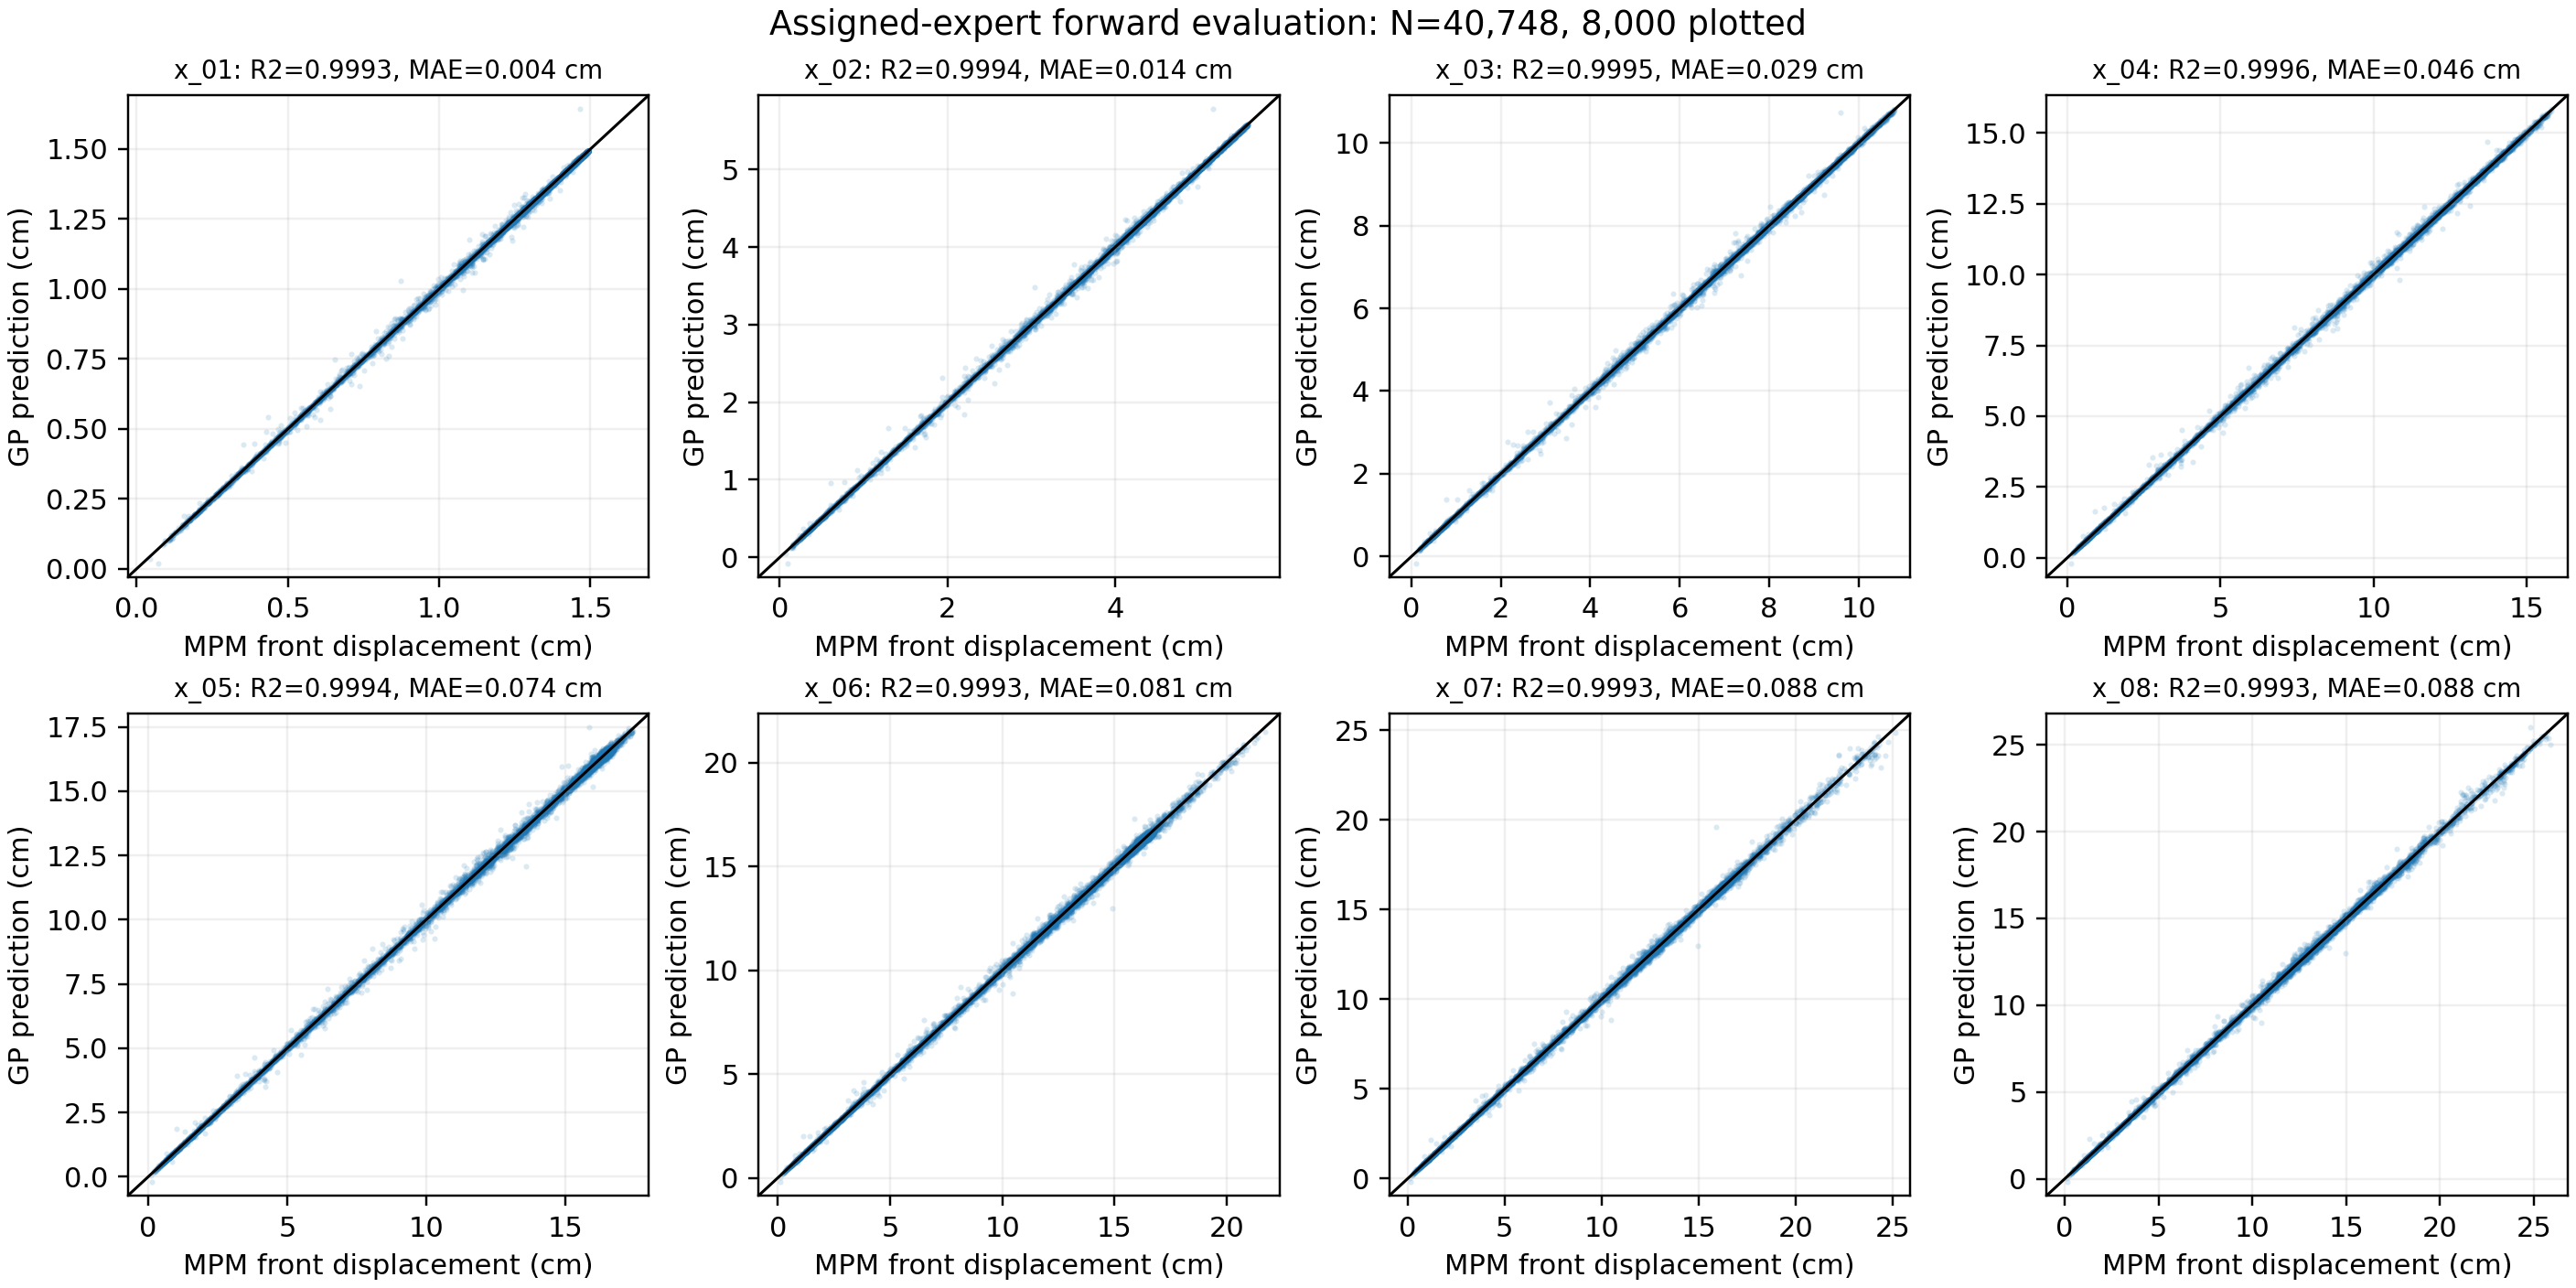
\includegraphics[width=\textwidth]{figs/true_vs_pred_current_gp.png}
\caption{Assigned-expert predictions versus simulated fronts at eight
frames. Metrics use all 40,748 test rows; 8,000 are displayed.
The response-informed partition is fixed before this checkpoint evaluation.}
\Description{Eight parity plots with a common simulated-versus-predicted
interpretation and per-frame errors.}
\label{fig:parity}
\end{figure*}

The bank supplies native GP variance and local BAE variance once to
the inverse. Local external-validation counts have minimum, median and
maximum $0/8/430$. The 40 validation-empty experts use the pooled
BAE fallback and are excluded from the 2,735-expert inverse pool.
For frame 8, pooled residual mean, standard deviation and absolute
p95 are $-0.00070$\,cm, $0.13782$\,cm and $0.28195$\,cm.
No residual mean is fitted online. The variance allowances are not
independently calibrated confidence intervals for material parameters.

The parity plots compare simulator trajectories, not camera measurements.
Synthetic recovery, rheometer agreement, observed-setup direct simulation
and third-setup images assess the remaining links separately.


\subsection{Validation with Synthetic 3D Emulations}
\label{sec:mainresults}

Synthetic observations supply parameter truths by construction.
The experiment tests whether small observed-front residuals imply
accurate flow curves or parameter triples under specified observation
perturbations. The simulator, inverse objective, budget and output
rules are those of the reported continuous method.



\subsubsection{Two-Setup Recovery Under Observation Perturbations}
\label{sec:continuous-synthetic}
The completed panel contains 40 triples drawn from rows of the fixed
forward corpus's held-out split, restricted to $n\in[0.3,1]$,
$\eta\in[1,300]$ and $\sigma_Y\in[1,400]$ in CGS.
For each material, two geometries are drawn uniformly from
$[2,7]^2$\,cm, at least 1.5\,cm apart in Euclidean geometry distance.
The fixed-density MLS simulator generates new eight-frame trajectories
at those geometries. Pairs with nonfinite output or maximum displacement
below 0.3\,cm in both setups are rejected and recorded.
This conditional sampling does not cover the full smallest-value
tails or the exact zero-yield limit.

\paragraph{Synthetic observation construction.}
Let $\mathbf x_j$ be a clean simulated trajectory.
A shared shift $\delta_j$ moves all sample times of setup $j$ by the
same fraction of a frame. Between samples, shape-preserving piecewise
cubic interpolation is applied after appending $x_j(0)=0$;
beyond frame 8 the final interval slope is extrapolated.
Writing the resulting trajectory as $\mathbf x_j^{\delta_j}$,
\[
 y_{j,d}=(1+\beta_j)x_{j,d}^{\delta_j}+\epsilon_{j,d},\qquad
 \beta_j\sim\mathcal N(0,0.03^2),
\]
\[
 \epsilon_{j,d}\sim\mathcal N\!\left(0,\,
 (0.02|x_{j,d}^{\delta_j}|)^2+(0.02\,\mathrm{cm})^2\right).
\]
The shift is drawn from $\mathcal N(0.2,0.4^2)$ frames and clipped
to $[-0.9,1.0]$ frames. Its scale was motivated by observed freshness
setup residual analyses. This is a development noise scenario rather
than an independently measured experimental law, and differs from
the solver's per-interval timing approximation.
The clean curves, shifts, scale biases and injected noise are stored
alongside the material truth.

The shifted condition contains 40 distinct parameter triples.
A paired control removes the time shift from 24 of them while
retaining the same geometries, multiplicative biases and realised
additive-noise vectors. Noise is not resampled or rescaled.
Thus 64 fits concern 40 parameter truths; the no-shift row is not
an independent material collection. All cases have been inspected
during development, so the panel is not an untouched generalisation test.

\paragraph{Fit and recovery.}
The evaluated protocol uses the reported continuous objective and
restart-output selection, without feasible-history retention, extra
feasibility refinement, expert mixing, or online physical simulation.
For synthetic truth, Eq.~\eqref{eq:E} is evaluated with
$\tau_{\rm ref}=\tau^\star$ on 101 rates from 1 to
100\,$\mathrm{s}^{-1}$; denote it by $E_{\rm flow}^{[1,100]}$.
The companion $E_{\rm flow}^{[3,30]}$ uses the same RMS natural-log
stress ratio on 51 geometrically spaced rates from 3 to
30\,$\mathrm{s}^{-1}$. Neither interval is asserted to equal the
shear-rate range uniquely identified by dam-break motion.

The parameter-error columns use $\Delta n=\hat n-n^\star$,
$|\Delta\ln\eta|=|\ln(\hat\eta/\eta^\star)|$, and
$|\Delta\ln\sigma_Y|=|\ln(\hat\sigma_Y/\sigma_Y^\star)|$.
The positive parameters are compared in the same fixed CGS convention;
these logarithmic ratios quantify multiplicative parameter errors.

\begin{table*}[!htbp]
\centering\footnotesize
\setlength{\tabcolsep}{4pt}
\caption{Two-setup recovery under observation perturbations. Both raw-fit-review cases remain in the recovery summaries. The no-shift control repeats 24 of the 40 parameter truths; fit counts are not independent material counts.}
\label{tab:continuous-synthetic}
\begin{tabular}{@{}lrrrrrrrr@{}}
\toprule
Observation condition & Fits & No estimate & Accepted & $E_{\rm flow}^{[1,100]}$ p50 / mean & $E_{\rm flow}^{[3,30]}$ p50 / mean & $|\Delta n|$ p50 & $|\Delta\ln\eta|$ p50 & $|\Delta\ln\sigma_Y|$ p50 \\
\midrule
Shifted observations & 40 & 0 & 38 & 0.379 / 0.545 & 0.352 / 0.480 & 0.163 & 0.751 & 2.811 \\
Paired subset, no shift & 24 & 0 & 24 & 0.232 / 0.279 & 0.160 / 0.221 & 0.164 & 0.830 & 1.761 \\
\bottomrule
\end{tabular}
\end{table*}

All 64 inputs return supported estimates; 62 pass the raw-fit gate.
For the 40 shifted inputs, median worst-setup relative RMSE is 0.071,
but median curve error is 0.379 and median yield-stress log-ratio
error is 2.811. Passing a proxy-fit gate therefore does not certify
parameter recovery. Within the paired 24-case subset, removing the
time shift lowers median wide-interval curve error from 0.362 to 0.232.
The comparison concerns the specified perturbations; it does not
identify a real video's time origin or establish a unique HB triple.



\subsubsection{Next-Setup Implementation Checks}
\label{sec:setup-validation}
The acquisition module in Sec.~\ref{sec:proposer} has two validation
questions: whether its inherited numerical rule is implemented
consistently, and whether the resulting extra observation improves
material recovery. Numerical availability alone cannot answer the
second question.

\paragraph{Implementation consistency and repair scope.}
For 338 estimates with a valid physical mapping, the proposed
geometry agrees case by case with an independent transcription of
the public Hamamichi rule. The availability audit evaluates 624
estimation-derived inputs and 600 random parameter/geometry inputs,
including extra small-consistency cases. All 1,224 return a proposal;
508 require common-offset continuation. Four independent numerical
formulations select the same geometry in all 508 continuation cases.
These checks establish numerical availability on the audited inputs,
not calibrated mapping physics or GP support at every proposal.

These checks concern numerical consistency and availability of the
optional proposal. They do not establish that its physical mapping is
calibrated, that every recommended geometry has surrogate support, or
that this rule improves recovery over a random design. The formal
real-material and fast freshness estimates use fixed geometries;
their performance does not validate an adaptive acquisition loop.

\subsection{Validation with Real-World Experiments}
\label{sec:rheometer}

This experiment tests whether parameters inferred from measured dam-break
trajectories agree with an independent constitutive reference. The six
materials are Chuno sauce, Okonomiyaki sauce, moisturising milk, lotion,
pork-cutlet sauce, and sweet bean paste. They differ from the six materials
in the freshness application. For each material, we evaluate the first
setup alone, the second setup alone, and their joint estimate. This design
separates fit to an observed transient from agreement with a rheometer,
and tests the value and limitations of combining physical conditions.

\subsubsection{Continuous Inference on the Measured Setup Pairs}
The two measured geometries in Tab.~\ref{tab:rheo-recovery} and their
eight-frame metric trajectories are fixed inputs. The continuous inverse
uses the frozen forward bank, expert-selection rules, marginal objective,
CMA-ES budget, and raw-fit reporting of Secs.~\ref{sec:retrieval}
and~\ref{sec:inverse}. No material-specific representative selection,
rheometer curve, or image-replay error changes its returned estimate.
The geometry pairs were acquired previously; this experiment does not
implement the adaptive recommendation loop of Sec.~\ref{sec:proposer}.

The observation audit reconstructed all twelve trajectories from their
saved masks and camera configurations and matched the 96 stored
displacements to numerical precision. This checks extraction under the
stored calibration, rather than independently certifying its physical
accuracy or identifying the original camera-fitting branch. For the
continuous runs, the ordered observation files, extracted-array hashes,
source snapshot, and protocol are bound to the saved numerical outputs.
All eighteen single-setup and joint estimates use the same forward bank
and error assumptions.

\paragraph{Rheometer reference and evaluation interval.}
The rotational-rheometer sweeps span $0.1$--$1000\,\mathrm{s}^{-1}$.
The stored reference HB parameters were fitted to fourteen sweep samples
over $1$--$398\,\mathrm{s}^{-1}$ by nonlinear least squares in shear
stress, with nonnegative bounds on consistency and yield stress and
$0\leq n\leq1$. All six fitted references have strictly positive
consistency, yield stress, and exponent.
These reference fits describe the rheometer data under the HB family;
they are not synthetic ground-truth material parameters.

The primary flow discrepancy is $E_{\rm flow}$ of Eq.~\eqref{eq:E}:
the RMS natural logarithm of predicted-to-reference HB stress on 101
log-spaced rates from $1$ to $100\,\mathrm{s}^{-1}$. This interval is
distinct from the wider measured sweep and reference-fitting interval.
The metric does not enter optimisation or output selection.

\begin{table*}[!htbp]
\centering\footnotesize
\setlength{\tabcolsep}{5pt}
\caption{Two-setup continuous estimates on six rheometer-reference materials. Geometries are $(W,H)$ in cm; $\hat n$ is dimensionless, $\hat\eta$ is in $\mathrm{Pa\,s}^{\hat n}$ and $\hat\sigma_Y$ in Pa. All joint fits pass the observed-front gate. External curve errors are reported separately in Table~\ref{tab:real-flow-stage-comparison}.}
\label{tab:rheo-recovery}
\begin{tabular}{@{}lccccc@{}}
\toprule
Material & $(W_1,H_1)$ & $(W_2,H_2)$ & $\hat n$
 & $\hat\eta$ & $\hat\sigma_Y$ \\
\midrule
Chuno & $(2.5,2.7)$ & $(4.0,2.0)$ & 0.739850 & 0.445357 & 6.713774 \\
Okonomiyaki & $(2.2,2.5)$ & $(7.0,7.0)$ & 0.338356 & 13.020025 & 0.163128 \\
Moisturising milk & $(4.5,3.5)$ & $(4.5,2.0)$ & 0.305020 & 6.187268 & 11.240282 \\
Lotion & $(6.1,2.8)$ & $(7.0,6.5)$ & 0.919571 & 1.239826 & 20.268173 \\
Pork-cutlet sauce & $(6.5,2.1)$ & $(7.0,7.0)$ & 0.686133 & 0.988307 & 7.834970 \\
Sweet bean paste & $(4.8,4.1)$ & $(2.5,2.5)$ & 0.857275 & 6.292245 & 33.384066 \\
\bottomrule
\end{tabular}
\end{table*}

\paragraph{Single versus joint estimates.}
The mean $E_{\rm flow}$ is $0.280483$ for setup~1, $0.671716$ for
setup~2, and $0.271667$ for the joint inverse
(Tab.~\ref{tab:real-flow-stage-comparison}). The joint estimate improves
over setup~1 for four materials, but is worse for Chuno and moisturising
milk. Relative to the better of the two individual fits, it is also
worse for sweet bean paste. Selecting the better individual fit with
the rheometer would use the evaluation reference to make an inverse
decision; we therefore report both individual results and consistently
draw setup~1 as the single-setup curve. The second setup is neither
silently substituted for setup~1 nor selected separately for each material.

All eighteen stages pass the proxy raw-fit gate. For the six joint fits,
the per-setup relative RMSE ranges from $0.0177$ to $0.0905$, below
the common threshold $0.20$. In spite of those accepted fits, the
joint flow discrepancy ranges from $0.106578$ to $0.534329$.
This distinction is central: agreement with eight front displacements
does not establish agreement with the full constitutive flow curve.
The joint moisturising-milk and lotion estimates are flagged near a
selected parameter-box boundary; this is a numerical-domain diagnostic,
not by itself proof of non-identifiability or incorrect physics.

\begin{table}[!htbp]
\centering\footnotesize
\setlength{\tabcolsep}{4pt}
\caption{External flow-curve error $E_{\rm flow}$ for each individual and joint estimate. All columns use the same inverse protocol, rheometer HB reference and 101-rate grid. Lower is better; these are log-stress RMS values, not percentages.}
\label{tab:real-flow-stage-comparison}
\begin{tabular}{@{}lrrr@{}}
\toprule
Material & Setup 1 & Setup 2 & Joint \\
\midrule
Chuno & 0.466053 & 0.292016 & 0.534329 \\
Okonomiyaki & 0.132814 & 1.377618 & 0.106578 \\
Moisturising milk & 0.283706 & 0.232754 & 0.291679 \\
Lotion & 0.243308 & 1.083810 & 0.219834 \\
Pork-cutlet sauce & 0.215398 & 0.885328 & 0.160617 \\
Sweet bean paste & 0.341618 & 0.158772 & 0.316967 \\
\midrule
Mean & 0.280483 & 0.671716 & 0.271667 \\
\bottomrule
\end{tabular}
\end{table}



\begin{figure*}[!htbp]
    \centering
    \begin{minipage}[t]{0.32\textwidth}
        \centering
        \figureorplaceholder[2.45cm]{\linewidth}{outputs/current_method_20261001/real6_Chuno.pdf}{(a) Chuno: measured rheometer sweep, setup-1 inverse, and joint inverse.}\\
        {\footnotesize (a) Chuno (Japanese thickened sauce)}
    \end{minipage}\hfill
    \begin{minipage}[t]{0.32\textwidth}
        \centering
        \figureorplaceholder[2.45cm]{\linewidth}{outputs/current_method_20261001/real6_Okonomiyaki.pdf}{(b) Okonomiyaki: measured rheometer sweep, setup-1 inverse, and joint inverse.}\\
        {\footnotesize (b) Okonomiyaki (cabbage pancake sauce)}
    \end{minipage}\hfill
    \begin{minipage}[t]{0.32\textwidth}
        \centering
        \figureorplaceholder[2.45cm]{\linewidth}{outputs/current_method_20261001/real6_MoisturizingMilk.pdf}{(c) Moisturising milk: measured rheometer sweep, setup-1 inverse, and joint inverse.}\\
        {\footnotesize (c) Moisturising milk}
    \end{minipage}\\[4pt]
    \begin{minipage}[t]{0.32\textwidth}
        \centering
        \figureorplaceholder[2.45cm]{\linewidth}{outputs/current_method_20261001/real6_Lotion.pdf}{(d) Lotion: measured rheometer sweep, setup-1 inverse, and joint inverse.}\\
        {\footnotesize (d) Lotion}
    \end{minipage}\hfill
    \begin{minipage}[t]{0.32\textwidth}
        \centering
        \figureorplaceholder[2.45cm]{\linewidth}{outputs/current_method_20261001/real6_Tonkatsu.pdf}{(e) Pork-cutlet sauce: measured rheometer sweep, setup-1 inverse, and joint inverse.}\\
        {\footnotesize (e) Japanese pork-cutlet sauce}
    \end{minipage}\hfill
    \begin{minipage}[t]{0.32\textwidth}
        \centering
        \figureorplaceholder[2.45cm]{\linewidth}{outputs/current_method_20261001/real6_SweetBeanPaste.pdf}{(f) Sweet bean paste: measured rheometer sweep, setup-1 inverse, and joint inverse.}\\
        {\footnotesize (f) Sweet bean paste}
    \end{minipage}
    \caption{Flow-curve validation of the continuous surrogate inverse
    on six real materials. Black dotted lines show the measured
    rheometer sweeps, red lines the setup-1 estimates, and blue lines
    the estimates jointly fitted to setups 1 and 2. In the inherited
    axis notation, $\sigma_s$ denotes the scalar shear stress $\tau$
    used in the HB law. Each existing panel uses logarithmic axes,
    the same rate and stress limits, and the same serif mathematical
    typography. The reference HB fits supply the numerical errors in
    Tab.~\ref{tab:real-flow-stage-comparison}; a separate HB-fit curve
    is not drawn. The plotting parameters equal the eighteen formal
    stage estimates. Setup~2 results are tabulated rather than used
    to choose the red curve. There is no real-domain representative
    selector between the inverse output and these curves.}
    \Description{Two rows of three log-log plots. Each shows black
    dotted rheometer measurements, a red setup-1 HB curve, and a blue
    joint HB curve for one real material.}
    \label{fig:flow-real}
\end{figure*}

The flow curves use the saved formal estimates and preserve the
black dotted/red/blue, log-axis and serif mathematical conventions.
Formal joint fits take $13.058$--$25.241$\,s under the scope in
Sec.~\ref{sec:timebudget}. Image-space validation of these real-material
estimates would require their own parameter-matched simulations,
camera configurations and masks; the flow-curve comparison alone does
not provide that validation.

\subsubsection{Reference-Model Shear-Rate Regimes}
A rheometer flow curve and a dam-break video sample a material in
different regimes. The rheometer imposes controlled, approximately steady
shear rates, whereas the dam-break experiment produces a transient,
spatially heterogeneous free-surface flow. Agreement with a rheometer
flow curve therefore should not be interpreted uniformly over the entire
sweep; the relevant question is which shear-rate regimes are excited by
the real validation setup
~\citep{balmforth2007two,pashias1996fifty,ahmadi2022identification,muchiri2024identification}.

The regime diagnostic replays each measured setup using the HB fit
to the rheometer sweep as a reference material. It records equivalent
shear rate $\dot\gamma_{\mathrm{eq}}=\sqrt{2D:D}$ over eight frames,
takes nonzero-particle quantiles per frame, then the temporal median
of each quantile. Figure~\ref{fig:gammadot-real} describes the
reference simulator's shear-rate support in those experimental
geometries. It uses no inverse candidate parameters and is not a
video measurement of shear rate.

The reference-model regime diagnostic uses MLS-MPM at
$\rho=1.025\,\mathrm{g\,cm}^{-3}$ and time step
$7.5\times10^{-5}$\,s, whereas the surrogate corpus uses
$\rho=1.0\,\mathrm{g\,cm}^{-3}$. This distinct reference condition
must be retained when interpreting the plotted support. The diagnostic
does not validate the continuous inverse's returned parameters or
equate the density assumptions of the two simulations.

For a local velocity field $\mathbf v$, the tensor
$D=(\nabla\mathbf v+\nabla\mathbf v^\top)/2$ measures the symmetric
rate of deformation. The scalar $\sqrt{2D:D}$ of
Eq.~\eqref{eq:hb-equivalent-scalars} equals the imposed rate in simple
shear but varies over particles and time in the dam break. It is the
kinematic equivalent rate, rather than the plastic-relaxation rate
$\dot\gamma_{\rm HB}$ of Eq.~\eqref{eq:hb-yield-flow}.
The transition scale follows by equating the reference HB yield and
rate-dependent stress contributions,
$\sigma_{Y,\rm ref}=\eta_{\rm ref}(\dot\gamma^\star)^{n_{\rm ref}}$,
giving Eq.~\eqref{eq:gammastar}. The ratio of their relative stress
sensitivities is $(\dot\gamma^\star/\dot\gamma)^{n_{\rm ref}}$
as derived in Eq.~\eqref{eq:ridge}; the yield contribution becomes
relatively weaker at high rates. This local constitutive argument
explains the diagnostic's purpose without proving identifiability
from a transient video.

We interpret this support through the HB transition scale
$\dot\gamma^\star=(\sigma_Y/\eta)^{1/n}$ from
Eq.~\eqref{eq:gammastar}. Setup pairs that sample both the
yield-sensitive and viscous/power-law-dominated regimes can provide
complementary information about $\sigma_Y$ and $(\eta,n)$. In contrast,
two setups whose shear-rate distributions remain in the same regime
provide more redundant information and may leave a continuum of
near-equivalent HB parameters.

The combined dam-break support summaries in Tab.~\ref{tab:gammadot-real} all lie
inside the measured rheometer interval $0.1$--$1000\,\mathrm{s}^{-1}$,
but they occupy only a subset of that interval. Thus flow-curve
agreement should be read most strongly over the overlap between the
rheometer sweep and the dam-break shear-rate support. Agreement outside
that support is a post-hoc HB extrapolation diagnostic rather than
direct video-supported validation. The setup pairs in this audit are
the measured real-material validation setups used by the inverse, not
pairs selected to maximise $\dot\gamma$ coverage; a separate
candidate-setup sweep would be required to claim maximal shear-rate
coverage.

\begin{table}[!htbp]
\centering
\footnotesize
\setlength{\tabcolsep}{4pt}
\caption{Dam-break shear-rate support under the rheometer-reference HB
material model. For each real material, the two measured validation
setups are replayed using the HB fit to the rheometer sweep, and
$\dot\gamma_{\mathrm{eq}}=\sqrt{2D:D}$ is summarised from nonzero
particle values. For each setup, take the temporal median of each
framewise p5, p50 and p95; across the two setups, report the minimum
p5 summary, the geometric mean of the p50 summaries, and the maximum
p95 summary. These are combined support descriptors, not quantiles
of a pooled particle--frame sample. These
values bound the interpretation of the flow-curve overlays; they do not
imply maximal setup coverage or validation of the entire rheometer
sweep. All three columns are in $\mathrm{s}^{-1}$.}
\label{tab:gammadot-real}
\begin{tabular}{@{}lccc@{}}
\toprule
Material & $\dot\gamma_{p5}$ & $\dot\gamma_{p50}$ &
$\dot\gamma_{p95}$ \\
\midrule
Chuno              & $1.70$ & $11.54$ & $35.99$ \\
Okonomiyaki        & $0.30$ & $4.88$  & $35.63$ \\
Moisturising milk  & $0.18$ & $4.58$  & $26.34$ \\
Lotion             & $0.17$ & $5.16$  & $33.98$ \\
Pork-cutlet sauce  & $0.36$ & $7.88$  & $63.89$ \\
Sweet bean paste   & $0.11$ & $1.95$  & $6.99$ \\
\bottomrule
\end{tabular}
\end{table}

\begin{figure*}[!htbp]
    \centering
    \begin{tabular}{ccc}
        \figureorplaceholder[2.45cm]{0.30\textwidth}{outputs/gamma_color_alignment_20261028/gamma_Chuno.png}{(a) Chuno shear-rate histogram.} &
        \figureorplaceholder[2.45cm]{0.30\textwidth}{outputs/gamma_color_alignment_20261028/gamma_Okonomiyaki.png}{(b) Okonomiyaki shear-rate histogram.} &
        \figureorplaceholder[2.45cm]{0.30\textwidth}{outputs/gamma_color_alignment_20261028/gamma_MoisturizingMilk.png}{(c) Moisturising milk shear-rate histogram.}\\
        \figureorplaceholder[2.45cm]{0.30\textwidth}{outputs/gamma_color_alignment_20261028/gamma_Lotion.png}{(d) Lotion shear-rate histogram.} &
        \figureorplaceholder[2.45cm]{0.30\textwidth}{outputs/gamma_color_alignment_20261028/gamma_Tonkatsu.png}{(e) Japanese pork-cutlet sauce shear-rate histogram.} &
        \figureorplaceholder[2.45cm]{0.30\textwidth}{outputs/gamma_color_alignment_20261028/gamma_SweetBeanPaste.png}{(f) Sweet bean paste shear-rate histogram.}
    \end{tabular}
    \caption{Shear-rate coverage of the real validation setups.
    Histograms show $\log_{10}\dot\gamma_{\mathrm{eq}}$ for the
    rheometer-reference material replayed in the two setup geometries
    used by the real experiments. Red denotes setup~1 and blue denotes
    setup~2, using the red/blue palette of Fig.~\ref{fig:flow-real}.
    In that flow-curve figure, blue denotes the joint estimate from both
    setups; the blue histogram here describes the second geometry alone.
    The gray interval marks the
    rheometer-measured shear-rate range, dashed vertical lines mark the
    HB-fit interval used for flow-curve comparison, and the horizontal
    bars below the curves show each setup's p5--p95 interval. The HB
    transition scale is interpreted in the text and is not drawn.
    These plots audit the
    reference-model shear-rate support for the video geometries; they are not histograms of
    the inverse candidate parameters.}
    \Description{Six log-shear-rate histograms showing that the
    dam-break support for setup 1 and setup 2 lies inside the
    rheometer-measured shear-rate interval for the real-material
    validation panel. Each plot identifies its material and the two
    measured geometries.}
    \label{fig:gammadot-real}
\end{figure*}

The reference-model distributions differ across the observed setups.
The setup median-rate separation is about $0.62$, $0.55$, and $0.71$
base-10 units for Okonomiyaki, lotion, and pork-cutlet sauce,
respectively; the corresponding separation is about $0.19$ for both
Chuno and sweet bean paste. The first group therefore excites more
distinct rate ranges under the reference model. This observation is
consistent with complementary constitutive information, but does not
establish that the corresponding transient inverse has full rank or
that adding a setup must improve its point estimate.

For Chuno, both setups mainly probe rates above the reference
transition scale, limiting their distinct information about a
yield-dominated response. Its continuous joint inverse has small
observed-front residuals but the largest real-material flow discrepancy.
For sweet bean paste, the combined p95 descriptor is only about
$7\,\mathrm{s}^{-1}$; agreement at substantially larger rates is
therefore an HB extrapolation diagnostic rather than direct support
from the dominant dam-break rate range. These are model-conditioned
interpretations. The histograms do not isolate the cause of the
remaining errors, which can also involve measurement error, simulator
discrepancy, surrogate coverage, and finite numerical search.



\subsection{Freshness-Oriented Sequential Measurement}
\label{sec:freshness}

\subsubsection{Question, preparation batches and observation roles}
Here, freshness concerns the temporal consistency of the material
represented by successive observations and the resulting estimate.
Simulation-in-the-loop estimation can impose hours of computation
before the next geometry is available. Continuing the sequence may then
require a newly prepared specimen; following the same preparation
procedure does not guarantee the same rheological response. A fast
inverse can reduce this computational waiting and the need to combine
captures across preparations. We examine the predictive behaviour and
recorded computation cost of these two practical workflows, rather
than defining a freshness parameter or identifying an ageing law.

The six materials are cream, custard, egg foam, potato-starch paste
(Katakuriko), oat paste, and yolk emulsion. They differ from the
rheometer-reference collection in Sec.~\ref{sec:rheometer}.
For each material, batch~A denotes the original preparation: setups~1,
2 and~3 were acquired close together from that batch. Batch~B denotes
a later, separately prepared specimen used for the simulation-based
workflow's supplementary setup~2. This preparation relationship was
confirmed by the experimenter. Exact preparation-to-capture intervals,
temperature histories and constitutive drift magnitudes were not
measured in this comparison. Batch labels identify specimen provenance;
they do not certify exactly constant HB parameters within a batch or
a known parameter change between batches.

The fast workflow fits the two stored front trajectories from
batch~A setups~1 and~2 using Sec.~\ref{sec:inverse}, freezes the
returned parameters, and predicts batch~A setup~3. The simulation-based
workflow reuses exactly the same first observation from batch~A,
performs the first-setup fit and setup-2 proposal, and acquires the
supplementary second observation from batch~B at the proposed geometry.
It then fits those two observations jointly and freezes the optimiser
library's returned parameters before predicting the same batch~A
setup~3. Figure~\ref{fig:fresh-workflow} separates these observation
sources from the later computation and scoring stages. The original
fast captures use their existing geometries; they did not consume the
simulation-based proposals.

\begin{figure*}[!htbp]
\centering
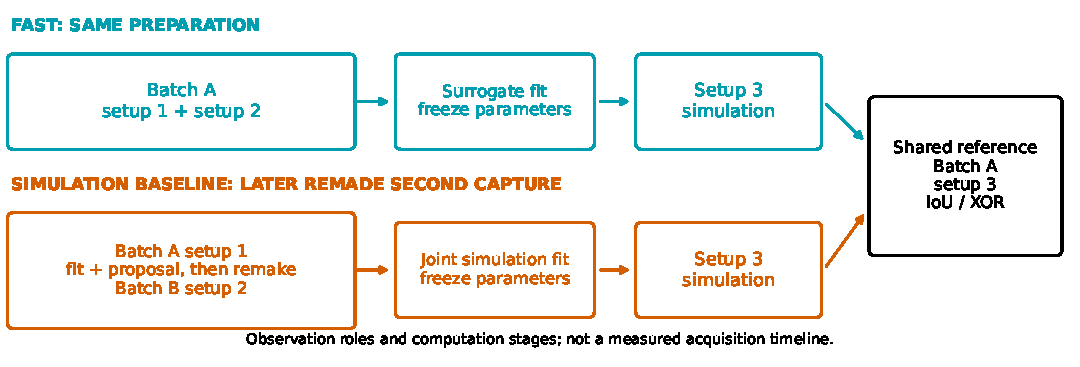
\includegraphics[width=0.98\textwidth]{figs/freshness_workflow_20261022/workflow_batches.pdf}
\caption{Observation roles in the freshness workflow comparison.
The original fast fit uses batch~A setups~1 and~2. The simulation-based
workflow uses the same batch~A setup~1, then a recommended setup~2
captured from a later, remade batch~B. Both returned parameter triples
are frozen before prediction at the common third geometry and scoring
against batch~A setup~3. The arrows show data dependencies, not a
measured acquisition timeline. Simulation does not create or change
the preparation batch of the recorded reference.}
\Description{Two routes with different second observations produce
frozen parameters, simulate the same third geometry, and compare with
one original-batch third observation.}
\label{fig:fresh-workflow}
\end{figure*}

Both joint fits still assume that one HB triple explains their two
inputs. If the remade specimen responds differently, the cross-batch
simulation-based estimate may be a compromise rather than the true
parameters of either preparation. The known batch difference does not
by itself measure that response change. The common third observation
tests prediction of batch~A, not prediction of a future batch~B capture.
Neither fit uses setup~3 in its objective, initialisation, parameter
selection or quality gate. Offline simulation dates do not change the
material state represented by the original recording, and fit-call
durations do not reconstruct the physical acquisition intervals.

\subsubsection{Frozen estimates and common third-setup evaluation}
Table~\ref{tab:fresh-holdout} retains the original fast parameters and
observed-setup fit states. The simulation-based stages and returned
parameters are reported in Sec.~\ref{sec:freshness-simulation-baseline}.
The second geometries differ as follows; the first input and third
evaluation geometry remain common within each material.

\begin{table}[!htbp]
\centering\small
\caption{Second-observation geometry $(W,H)$ in cm and preparation
source. The two columns are different captures, not alternative
processing of one video.}
\label{tab:fresh-second-geometries}
\begin{tabular}{@{}lll@{}}
\toprule
Material & Fast: batch A & Simulation: batch B \\
\midrule
Cream & $(6.0,2.0)$ & $(3.5,2.0)$ \\
Custard & $(6.0,2.5)$ & $(2.0,2.0)$ \\
Egg foam & $(7.0,7.0)$ & $(2.9,2.2)$ \\
Katakuriko & $(6.5,2.0)$ & $(2.0,2.0)$ \\
Oats & $(3.0,2.0)$ & $(2.3,2.0)$ \\
Yolk emulsion & $(7.0,5.2)$ & $(7.0,7.0)$ \\
\bottomrule
\end{tabular}
\end{table}

For setup~3, both predictions use identical observed masks, camera
parameters and geometry settings, and the same full-resolution scoring
rasteriser. Density $1.0\,\mathrm{g\,cm}^{-3}$ is a common modelling
assumption, not a measurement of each specimen's actual density.
The original fast replay uses the saved Windows uGIMP
implementation; the simulation-based replay uses the restored Linux
native chain. Shared recorded geometry, density and discretisation
settings do not establish bitwise equivalence of those implementations.
Together with the different second observations and inverse objectives,
this limits the comparison to the implemented workflows.

The unmodified $1920\times1080$ masks at frames~1--8 are scored using
the IoU and whole-image XOR definitions in
Sec.~\ref{sec:experimental-setup}. Each material score is its
eight-frame arithmetic mean; the panel mean weights all 48 frames
equally. Frame~0 and the supplementary second oat sequence are
excluded. No pixel-pooled aggregation or display crop changes a score.
All six outputs, including raw-fit-review estimates, remain in the
denominator. Parameters and source masks are not changed by this
comparison.

\begin{table*}[!htbp]
\centering\small
\setlength{\tabcolsep}{5pt}
\caption{Frozen two-setup freshness parameters and observed-front fit. Consistency and yield stress are in SI units; $E_1$ and $E_2$ are the relative RMSEs of Eq.~\eqref{eq:inverse-raw-relative-rmse}, shown as percentages. A dagger marks a raw-fit-review outcome retained in the third-setup evaluation in Table~\ref{tab:fresh-workflow-results}.}
\label{tab:fresh-holdout}
\begin{tabular}{@{}lrrrrr@{}}
\toprule
Material & $\hat n$ & $\hat\eta$ [Pa\,s$^{\hat n}$]
 & $\hat\sigma_Y$ [Pa] & $E_1$ [\%] & $E_2$ [\%] \\
\midrule
Cream & 0.421888 & 8.639542 & 17.001523 & 7.90 & 9.36 \\
Custard & 0.312045 & 27.038608 & 32.717517 & 6.77 & 17.93 \\
Egg foam & 0.999607 & 0.028926 & 0.000110 & 14.57 & 13.04 \\
Katakuriko$^\dagger$ & 0.590753 & 17.771245 & 13.459427 & 25.73 & 63.33 \\
Oats$^\dagger$ & 0.345508 & 29.684491 & 12.230795 & 7.75 & 22.46 \\
Yolk emulsion & 0.518600 & 19.184349 & 5.270152 & 2.25 & 2.09 \\
\bottomrule
\end{tabular}
\end{table*}

The 48-frame mean IoU is $0.9138190412$, with framewise median
$0.924592$ and minimum $0.805576$; mean whole-image XOR is
$0.00436332$. Tables~\ref{tab:fresh-holdout} and~\ref{tab:fresh-workflow-results} separate observed-front fit from third-setup mask agreement.
Katakuriko fails the raw-fit gate at both observed setups, and oats
fails it at the second, despite the oat replay's mean IoU of $0.956437$.
Their diagnostic parameters and replay scores remain reported, but
neither case is counted as an accepted inverse. The other four estimates
pass the surrogate raw-fit gate. Passing that gate does not establish
true HB parameter recovery, a unique constitutive fit, or independent
physical accuracy.


\paragraph{Main workflow comparison.}
Table~\ref{tab:fresh-workflow-results} compares the original fast
estimate with the completed simulation-based joint estimate on the
common batch~A setup~3. Mean IoU increases from $0.877112$ to
$0.913819$, a difference of about $3.67$ percentage points; mean
whole-image XOR decreases from $0.006449$ to $0.004363$.
The fast workflow has higher mean IoU and lower mean XOR for five
materials; egg foam is slightly better for the simulation-based
workflow. No material is removed on the basis of fit state or
third-setup performance.

\begin{table*}[!htbp]
\centering\small
\setlength{\tabcolsep}{7pt}
\caption{Main freshness workflow comparison on the same original-batch
third observation. Each entry averages frames~1--8 at full resolution;
the final row gives the 48-frame equal-weight mean. The simulation-based
fit combines batch~A setup~1 with remade-batch setup~2; the fast fit
uses batch~A setups~1 and~2. A dagger retains a fast raw-fit-review
outcome; it does not signify an accepted estimate.}
\label{tab:fresh-workflow-results}
\begin{tabular}{@{}lrrrrl@{}}
\toprule
 & \multicolumn{2}{c}{Mean IoU} & \multicolumn{2}{c}{Mean whole-image XOR} & \\
Material & Simulation & Fast & Simulation & Fast & Fast fit state \\
\midrule
Cream & 0.901224 & 0.955744 & 0.006709 & 0.002743 & Accepted \\
Custard & 0.889537 & 0.925007 & 0.002881 & 0.001824 & Accepted \\
Egg foam & 0.865286 & 0.859504 & 0.011161 & 0.011730 & Accepted \\
Katakuriko$^\dagger$ & 0.855454 & 0.879360 & 0.005442 & 0.004328 & Raw-fit review \\
Oats$^\dagger$ & 0.894278 & 0.956437 & 0.008878 & 0.003310 & Raw-fit review \\
Yolk emulsion & 0.856896 & 0.906862 & 0.003622 & 0.002245 & Accepted \\
\midrule
All six / 48 frames & 0.877112 & 0.913819 & 0.006449 & 0.004363 & Four accepted, two review \\
\bottomrule
\end{tabular}
\end{table*}

The error maps in Fig.~\ref{fig:fresh-binary} show how these aggregate
scores relate to shape. For cream and oats, the simulation-based
prediction increasingly extends beyond the observed right-hand and
lower boundary in later frames; the fast mismatch band is narrower.
Egg foam retains irregular upper-edge and lower-boundary errors in
both workflows, and its frame-8 ranking does not represent the
eight-frame mean. Yolk emulsion still has a visible fast-method
mismatch at the right boundary in frame~8. Improvements are therefore
neither uniform across frames nor present at every boundary location.
These residual shapes do not identify temperature, bubble or ageing
changes as their cause.

\paragraph{Direct-simulation check at the observed setups.}
An already completed offline check evaluates the frozen joint parameters
at both observed geometries with the separate MLS-MPM implementation.
The validation entry point fixes density to
$1.0\,\mathrm{g\,cm}^{-3}$ and passes the saved parameter triple,
$W$, and $H$ directly to the simulator; it does not reoptimise them.
The simulated fronts, GP means and measured trajectories are preserved
for all twelve setup queries.

For this check, $E_j^{\rm MLS}$ is the curve-energy-normalised RMSE of
Eq.~\eqref{eq:inverse-raw-relative-rmse} with the GP mean replaced by
the direct simulated eight-frame displacement. The GP--MLS discrepancy
is the unnormalised RMS difference between those two predicted
displacement vectors, in cm. These are observed-setup physical-forward
diagnostics, rather than third-setup mask scores.

\begin{table}[!htbp]
\centering\footnotesize
\setlength{\tabcolsep}{4pt}
\caption{Completed direct MLS checks of the frozen freshness parameters
at the two observed setups. $E_j^{\rm MLS}$ is dimensionless and shown
as a fraction. The last two columns are GP--MLS displacement RMS in cm.
No parameter or quality status is changed by this offline check.}
\label{tab:freshness-observed-mls}
\begin{tabular}{@{}lrrrr@{}}
\toprule
Material & $E_1^{\rm MLS}$ & $E_2^{\rm MLS}$
 & GP--MLS 1 & GP--MLS 2\\
\midrule
Cream & 0.0934 & 0.3217 & 0.1492 & 0.3351\\
Custard & 0.1074 & 0.2210 & 0.0778 & 0.0072\\
Egg foam & 0.1431 & 0.1183 & 0.0709 & 0.7498\\
Katakuriko & 0.3648 & 0.6534 & 0.3996 & 0.0410\\
Oats & 0.4270 & 0.2336 & 0.9780 & 0.0193\\
Yolk emulsion & 0.0381 & 0.0171 & 0.0183 & 0.0176\\
\bottomrule
\end{tabular}
\end{table}

Proxy fit, direct simulated front fit and held-out silhouette agreement
can differ substantially. Cream's second setup has GP relative RMSE
0.0936 but direct MLS relative RMSE 0.3217. Oats' first setup changes
from GP error 0.0775 to MLS error 0.4270, despite the third-setup
mean IoU of 0.9564. Consequently, a high held-out mask overlap cannot
substitute for observed-setup forward agreement, and a passing GP gate
does not guarantee that a physical replay passes the same numerical
error level. We retain the original proxy status rather than invent
a new acceptance classification from this check.

The diagnostics also have different simulator identities: the fixed
GP was trained on the offline CuPy/CUDA MLS-MPM corpus, this observed
check uses the separate headless MLS implementation, and the third-setup
image replay uses the uGIMP implementation. A GP--MLS
difference therefore need not be pure GP regression error relative to
an identical trajectory generator; numerical implementation differences
can contribute. These comparisons neither isolate all discrepancy
sources nor establish HB parameter uniqueness.
The direct checks and third-setup replays occur after parameter selection. They are
validation evidence, never an online filter or a means to choose
parameters, experts or thresholds.




\begin{figure*}[!htbp]
\centering
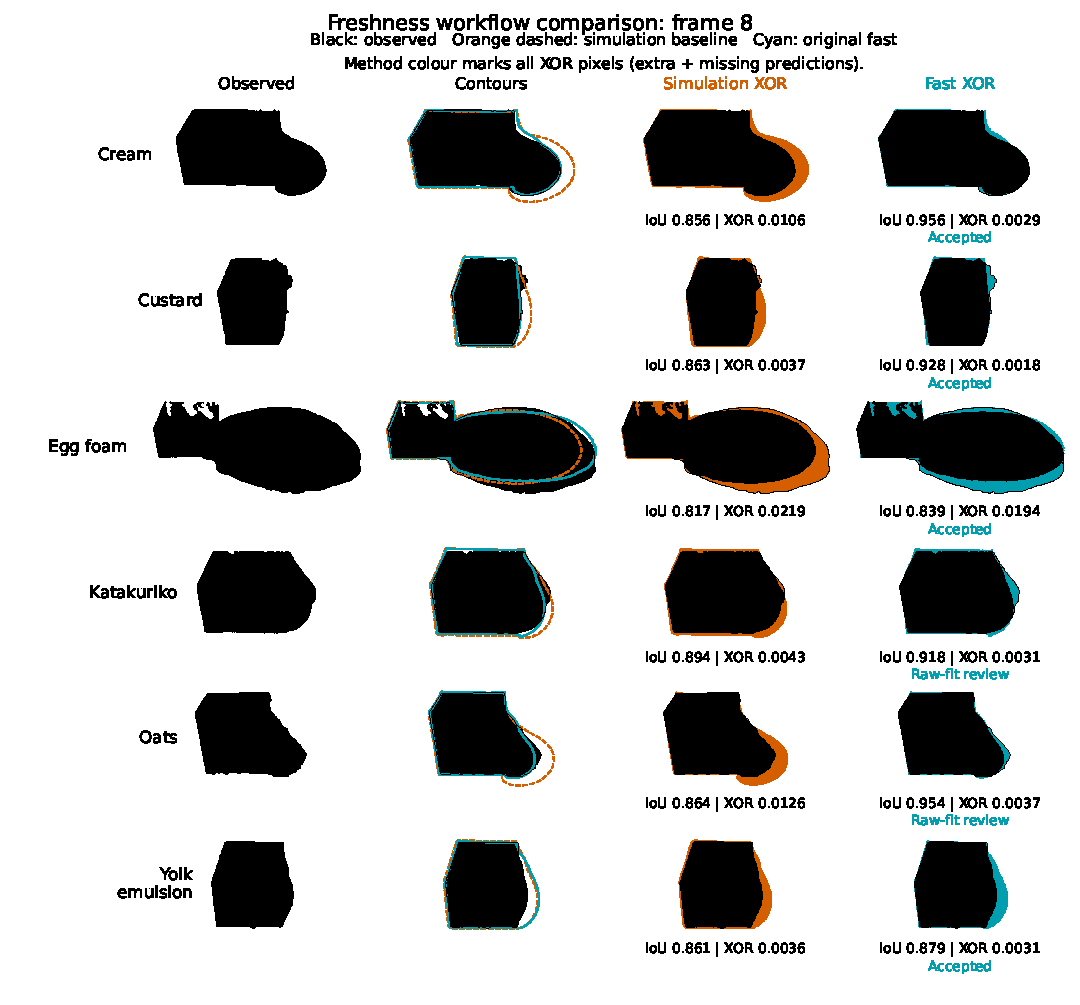
\includegraphics[width=0.98\textwidth,keepaspectratio]
 {figs/freshness_workflow_20261022/main_comparison_frame8_print.pdf}
\caption{Freshness workflow comparison on the third observation from
the original preparation batch. The fast estimate uses the first two
observations from that batch; the simulation-based estimate combines
the same first observation with a supplementary second observation
from a later, separately prepared batch. Rows show frame~8 for the six
materials. Columns are observation, contour overlay, simulation-based
mismatch and original fast mismatch. Observations are black, the
simulation-based baseline is orange (dashed in the overlay), and the
fast method is cyan (solid). Method-coloured pixels mark all silhouette
mismatches, including both extra and missing predictions. Displayed
scores refer to frame~8; Table~\ref{tab:fresh-workflow-results} averages
frames~1--8 at full resolution. Common display crops do not affect
scoring. No third-setup score selects a parameter or repairs a mask.
The comparison evaluates workflows with different second observations,
not a matched-input optimiser ablation.}
\Description{Six rows show black observed silhouettes, orange and cyan
contours, orange simulation-based XOR maps and cyan fast XOR maps.
Katakuriko and oats retain their raw-fit-review labels.}
\label{fig:fresh-binary}
\end{figure*}

Replay geometries are bound to the saved settings and cuboid
configuration: setup~3 has $H=3.5$\,cm for cream and $H=2.5$\,cm for
egg foam. They are common to both predictions and were not selected
by IoU. The third capture is excluded from fitting, but the material
panel was examined during development and is not an untouched external test.





\subsubsection{Completed simulation-based sequential baseline}
\label{sec:freshness-simulation-baseline}
To prepare a direct workflow comparison, the existing Linux
simulation-in-the-loop implementation was run on setup~1 of each of
the same six materials. This is a Linux port of the Hamamichi workflow,
using uGIMP, surface reconstruction, rendering and full-image XOR inside
CMA-ES. Its logarithmic parameter coordinates, platform adaptation and
static-boundary implementation differ from the original public Mac
implementation. It is therefore identified as the existing Linux
simulation-based baseline, not a byte-identical execution of the
authors' source or an isolated optimiser ablation.

The six runs retain population~7, seed~10, initial step size~1.0,
and a maximum of 100 generations. Each completed 700 candidate
evaluations and stopped on the generation budget. Completion means
the configured budget and output checks finished; it does not prove
numerical convergence or a globally optimal material estimate.
The primary parameter is the optimiser library's returned best member
of the final generation. The all-history minimum is preserved
separately and is not substituted after looking at its loss or
recommended geometry.

\begin{table*}[!htbp]
\centering\small\setlength{\tabcolsep}{5pt}
\caption{Single-setup simulation-based baseline parameters in SI units. All six fits stop at the 100-generation budget after 700 evaluations. XOR averages eight full $960\times540$ optimisation images. Second geometries and times appear only in Tables~\ref{tab:fresh-second-geometries} and~\ref{tab:fresh-workflow-time}.}
\label{tab:freshness-old-setup1}
\begin{tabular}{@{}lrrrr@{}}
\toprule
Material & $\hat n$ & $\hat\eta$ [Pa\,s$^{\hat n}$] & $\hat\sigma_Y$ [Pa] & XOR \\
\midrule
Cream & 0.535490 & 10.064747 & 2.933669 & 0.00800709 \\
Custard & 0.993918 & 23.446867 & 1.381154 & 0.00343967 \\
Egg foam & 0.999929 & 0.047807 & 0.001183 & 0.00960045 \\
Katakuriko & 0.999845 & 2.807416 & 34.487848 & 0.00498264 \\
Oats & 0.997304 & 5.730819 & 1.519945 & 0.00450424 \\
Yolk emulsion & 0.699627 & 20.954466 & 0.495047 & 0.00147401 \\
\bottomrule
\end{tabular}
\end{table*}

The setup-1 estimates supply the second geometries in
Table~\ref{tab:fresh-second-geometries}. All six proposals use the
criterion in Sec.~\ref{sec:proposer} without mapping continuation;
surrogate coverage at these proposals is not certified. The subsequent
joint simulation-based fits retain population 7, seed 10, initial
step $2/3$, native parameter bounds and the equal-weight mean of
the two eight-frame XOR objectives. Each completes 700 evaluations
and stops at the 100-generation budget, rather than a certified optimum.
Returned parameters are fixed before common third-setup evaluation.

\begin{table*}[!htbp]
\centering\small
\setlength{\tabcolsep}{7pt}
\caption{Completed simulation-based joint estimates from original
setup~1 and remade-batch setup~2. Parameters are in SI units; the
returned candidate is the original optimiser-library output.
Joint XOR averages the two eight-frame means at the native
$960\times540$ optimisation resolution, not the third-setup score.
All runs stop at their configured 100-generation budget.}
\label{tab:freshness-old-joint}
\begin{tabular}{@{}lrrrr@{}}
\toprule
Material & $\hat n$ & $\hat\eta$ [Pa\,s$^{\hat n}$]
 & $\hat\sigma_Y$ [Pa] & Joint XOR \\
\midrule
Cream & 0.793190 & 4.932032 & 0.944775 & 0.00528706 \\
Custard & 0.971835 & 24.204166 & 0.805281 & 0.00251218 \\
Egg foam & 0.999926 & 0.050644 & $4.24098\!\times\!10^{-6}$ & 0.00723645 \\
Katakuriko & 0.472069 & 21.916761 & 1.995021 & 0.00284397 \\
Oats & 0.999826 & 5.507447 & 0.420321 & 0.00419874 \\
Yolk emulsion & 0.940810 & 1.647247 & 32.750411 & 0.00384922 \\
\bottomrule
\end{tabular}
\end{table*}

The final returned candidates in Table~\ref{tab:freshness-old-joint}
are not replaced by the all-history minimum-loss parameters. For
custard, the returned and lowest recorded losses coincide at native
text precision but their parameter vectors differ; for the other
five materials the returned loss is slightly higher. The returned
parameters are the ones used for the common third-setup predictions
in Table~\ref{tab:fresh-workflow-results}. This evaluation does not
select an inverse output using the held-out images. Both workflows
use density $1.0\,\mathrm{g\,cm}^{-3}$; the simulation-based native
optimisation images and XOR objective remain distinct from the fast
front-displacement representation and marginal objective.

\subsubsection{Interpretation and further attribution controls}
\label{sec:freshness-future-protocol}
The completed comparison combines an original same-preparation
observation sequence with a later remade-batch supplementary capture.
It is not a new, synchronised, randomly assigned trial of two complete
acquisition schedules. The known batch provenance and recorded costs
make the practical state-consistency issue explicit, while the
common-target scores quantify predictive behaviour on the original
preparation. They do not assign the entire score difference to waiting,
ageing or remaking: second geometry, acquisition variation, inverse
representation, surrogate error and numerical implementation can also
contribute. A cross-batch shared-HB fit remains a defined numerical
problem; its physical interpretation depends on whether the two
specimens actually share a response. No batch~B third observation is
evaluated here, so these scores do not establish the returned baseline
parameters' accuracy for future use on batch~B.

More specific causal attribution would require prespecified repeated
preparations or paired aliquots, explicit records of preparation,
capture, computation and manual-adjustment intervals, and a fixed
geometry measured early and late. Such controls would distinguish
material response changes from release and acquisition variation,
including materials with little drift and failed measurements.
Consistent numerical implementations and controlled second geometries
would further separate acquisition effects from estimation effects.
Those attribution controls have not been performed in this comparison.
They are distinct from the completed supplementary captures, joint
fits and third-setup predictions reported above, and are not inferred
from offline computation timestamps or silhouette residual shapes.

The supported conclusion is that the original fast same-batch workflow
has better average original-batch third-setup agreement in this
six-material collection, with substantially shorter recorded inverse
computation. This supports reducing computational waiting and reliance
on cross-preparation observations as a practical motivation. It is
not an identified ageing law, a proof of exact constant material state,
an isolated optimiser accuracy comparison, or a claim of HB parameter
uniqueness.


\FloatBarrier
\subsection{Compute-Stage Time Budget}
\label{sec:timebudget}

\paragraph{Frozen result-producing runs.}
We separate per-fit inverse time from initial forward-interface
construction, measurement construction, setup proposal and physical
replay. The saved wall timer brackets the complete fit call: it includes
observation-conditioned expert selection, numerical search, returned-point
reevaluation, validity and raw-fit assessment, and construction of the
in-memory result. It excludes initial forward-interface construction
and the subsequent outer per-case JSON serialisation and file write,
as well as video capture, calibration, segmentation, MPM simulation
and rendering. Individual experts can be loaded lazily inside a fit;
that cost and the sequentially evolving expert-cache state remain as
recorded. No separate sensitivity or refinement diagnostics were enabled
in this frozen protocol. Table~\ref{tab:time-budget} reports those
single-run measurements for the real-material estimates. Freshness
measurements are reported separately in Table~\ref{tab:fresh-workflow-time}. They are observed run costs, not
three-repeat controlled latency distributions.

\begin{table*}[!htbp]
\centering\small
\setlength{\tabcolsep}{4pt}
\caption{Real-material inverse-call wall times in seconds. Each row reports two individual fits and their joint fit. Lazy expert loading and in-call cache effects are included; initial forward construction, outer file writing, acquisition and physical replay are excluded.}
\label{tab:time-budget}
\begin{tabular}{@{}lrrr@{}}
\toprule
Material & Setup 1 & Setup 2 & Joint \\
\midrule
Chuno & 11.751 & 2.905 & 17.407 \\
Okonomiyaki & 15.289 & 3.475 & 18.881 \\
Moisturising milk & 2.466 & 6.950 & 13.058 \\
Lotion & 8.207 & 3.919 & 25.241 \\
Pork-cutlet sauce & 4.219 & 5.143 & 18.998 \\
Sweet bean paste & 4.404 & 11.787 & 19.923 \\
\bottomrule
\end{tabular}
\end{table*}

The frozen real-material joint fits span $13.058$--$25.241$\,s,
and the six freshness joint fits span $5.192$--$25.409$\,s.
The complete real-material batch takes $197.762$\,s for its 18 fit
stages including loading and batch overhead; the six-fit freshness
batch takes $109.944$\,s on the same inclusive batch convention.
The latter cannot be divided into a single-setup latency, nor compared
directly with the setup-1 simulation queue to obtain a matched speedup.
The saved environment binds the package and source versions, but these
original runs were not a hardware-normalised, interleaved benchmark.
The supported statement is seconds-scale inversion for the recorded
workloads, with the stated loading and measurement exclusions.

\paragraph{Physical replay and simulation-based optimisation costs.}
In the same frozen freshness packet, simulation of one fixed material
at its third geometry takes $71.290$--$156.930$\,s and rendering takes
$19.466$--$50.120$\,s. These are offline checks of already selected
parameters; neither enters the online inverse timer. In contrast, the
Linux baseline in Table~\ref{tab:freshness-old-setup1} repeats simulation
and rendering inside each setup-1 objective evaluation. Its per-material
wall cost is $3.623$--$7.844$\,h, on a single sequential GPU queue under
WSL2 with an NVIDIA RTX~5060~Ti. Those times include external checks
and cleanup, and the optimisation image resolution, objective, parameter
coordinates and workload differ from the surrogate runs. They establish
a substantial practical computation burden for that implemented
workflow, but do not yet establish a matched-accuracy or
matched-observation speedup factor.

\begin{table*}[!htbp]
\centering\small
\setlength{\tabcolsep}{7pt}
\caption{Computation records bound to the freshness estimates in the
main comparison. Simulation-based stages include native simulation,
rendering, external per-candidate checks and cleanup; fast joint fits
use the inverse-call scope of Table~\ref{tab:time-budget}.
The two-stage sum excludes preparation, acquisition, manual waiting,
failed earlier attempts and third-setup replay. No matched fast
setup-1 timer is available here. Different platforms and included
overheads preclude interpreting these entries as a strict speedup ratio.}
\label{tab:fresh-workflow-time}
\begin{tabular}{@{}lrrrr@{}}
\toprule
 & \multicolumn{3}{c}{Simulation-based workflow [h]} & Fast [s] \\
Material & Setup 1 & Joint & Two-stage sum & Joint \\
\midrule
Cream & 7.844 & 10.756 & 18.600 & 20.043 \\
Custard & 6.330 & 8.326 & 14.656 & 5.192 \\
Egg foam & 3.623 & 6.691 & 10.315 & 24.511 \\
Katakuriko & 4.181 & 6.556 & 10.737 & 10.536 \\
Oats & 4.197 & 6.591 & 10.788 & 25.409 \\
Yolk emulsion & 3.654 & 12.622 & 16.276 & 21.631 \\
\bottomrule
\end{tabular}
\end{table*}

The six simulation-based joint records sum to $51.542$\,h; the six
fast fit calls sum to $107.322$\,s, or $109.944$\,s including the
original fast batch's loading and outer overhead. These are sums
over different tasks and timing scopes, not a matched sequential
acquisition latency. In particular, the fast joint timer does not
provide a full setup-1--proposal--setup-2 workflow timer. The
simulation-based first fit precedes its second-geometry proposal and
supplementary capture: its $3.623$--$7.844$\,h cost is therefore
directly relevant to retaining an original preparation for the next
measurement. The later joint fit adds $6.556$--$12.622$\,h; the
two recorded stages total $10.315$--$18.600$\,h per material.
The actual preparation and capture intervals are not recovered from
these computation times.

The reported costs distinguish model preparation, inverse calls,
optional geometry selection, acquisition and offline validation.
They support seconds-scale numerical fits for the measured workloads,
not end-to-end real-time operation or an accuracy-matched speedup.
The controls in Sec.~\ref{sec:freshness-future-protocol} are still needed
to isolate delay or material-change effects.\FloatBarrier

\section{Discussion and Limitations}
\label{sec:discussion}

The experiments assess several distinct links in video rheometry:
approximation of a simulated trajectory, numerical fitting of observed
fronts, agreement with an external flow curve, prediction at another
geometry, and the time needed to obtain an estimate. These links have
different references and failure modes. We interpret them separately
before considering what a fast inverse can contribute to a sequence of
physical measurements.

\subsection{Surrogate Fidelity and Inverse Identifiability}

The fixed GP bank makes repeated trajectory evaluation inexpensive,
but its assigned-expert MAE of $0.05297$\,cm does not certify inverse
recovery (Sec.~\ref{sec:fidelity}). The response-informed partition is
fixed in that forward evaluation; the online inverse preselects its
own supported expert combinations. Average forward error therefore
does not bound every parameter visited during optimisation, particularly
near support boundaries or where different HB triples have similar fronts.

The inverse combines local support checks with a working error
model. Its covariance contains native GP and BAE variance once,
plus absolute, relative, timing and shared scale-dependent bias terms.
The shared term uses one coefficient multiplied by the observation
scale, rather than a constant displacement. The marginal objective
includes a weighted residual and a log determinant
(Eq.~\eqref{eq:inverse-marginal-loss}). These allowances are assumptions,
not independently measured camera, simulator or release-time error
distributions; they do not provide calibrated parameter confidence.

The continuous inverse returns a parameter point with applicability
and fit information, or an explicit failure state
(Sec.~\ref{sec:inverse-output}). Its accepted state requires the raw
relative front RMSE to pass at every observed setup. This check prevents
a large working variance alone from disguising a poor front fit, but
does not establish constitutive accuracy. A review point is a reported
diagnostic outcome, not an accepted material identification. Supported
parameter boxes and local input distances limit extrapolation without
certifying a prediction-error bound. Likewise, a parameter near a
boundary flags proximity to the edge of the prescribed domain. That
flag by itself does not establish parameter unidentifiability. The bounded CMA-ES search supplies no
proof of a global minimum, and numerical stopping and budget exhaustion
remain distinct from parameter recovery.

The observation-perturbation panel makes this distinction concrete
(Sec.~\ref{sec:continuous-synthetic}). All 64 fits on 40 parameter
truths return supported estimates and 62 pass the raw gate.
The shifted condition has median flow error 0.379 and median
yield-stress log-ratio error 2.811 despite a median worst-setup
front RMSE of 0.071. Within the paired 24-case subset, removing the
imposed time shift lowers median flow error from 0.362 to 0.232.
These are specified synthetic perturbations, not an identification
of a real video's release time or an independent generalisation test.



Different HB triples may predict similar free-surface motion over
a limited excited shear-rate range. Additional geometries can supply
complementary observations~\cite{hamamichi2023nonnewtonian}, but joint
fitting also depends on state consistency and forward-model adequacy.
Local sensitivity or curvature diagnoses weak directions under stated
assumptions; it does not prove global uniqueness or calibrated intervals.

\subsection{Constitutive Agreement and Cross-Setup Prediction}

For six rheometer-reference materials, mean joint
$E_{\mathrm{flow}}=0.271667$ on $1$--$100\,\mathrm{s}^{-1}$;
the material-wise range is $0.106578$--$0.534329$
(Tab.~\ref{tab:real-flow-stage-comparison}). All eighteen single and
joint stages pass the proxy-fit gate. The external reference is an
HB fit to measured rheometer data, not known parameter truth.

Joint estimation improves on setup~1 for four materials, but worsens
for Chuno and moisturising milk. Relative to the better of the two
single-setup estimates, sweet bean paste also worsens. An additional
observation constrains the same parameter triple more strongly only
within the shared-state and forward-model assumptions. It can expose
inconsistency between observations or move a compromise estimate away
from the external reference. These outcomes demonstrate why a passing
observed-front fit is not a guarantee of better constitutive agreement
and why single-setup results must remain visible alongside the joint
estimate. They do not determine whether observation error, physical
model discrepancy, surrogate error, or finite numerical search is the
principal cause in a particular material.

The shear-rate audit provides a physical context for these comparisons
(Tab.~\ref{tab:gammadot-real} and Fig.~\ref{fig:gammadot-real}). Its
central support descriptors fall within the measured rheometer range,
but cover only part of it. They are summaries of particle rates
predicted using the rheometer-reference HB material, not shear rates
measured from the video or strict bounds on all particles and times.
The reference replay also uses density
$1.025\,\mathrm{g\,cm}^{-3}$, distinct from the surrogate's
$1.0\,\mathrm{g\,cm}^{-3}$. Relative to the HB transition scale
$\dot\gamma^\star$ of Eq.~\eqref{eq:gammastar}, predominantly high-rate
motion can constrain the rate-dependent contribution while providing
less information about the yield contribution. Agreement far outside
the modelled dam-break rate range is consequently an HB extrapolation
diagnostic. This interpretation does not establish an optimal setup
pair or prove the rank of the transient inverse problem.

The real-material flow curves do not provide parameter-matched
image-space validation. Such a test would need physical replays at
the exact returned estimates with matched geometry, camera and masks.
It remains distinct from the completed third-setup prediction on the
separate freshness collection.

For the separate freshness collection, the fast same-batch
estimates predict the excluded third observation with mean IoU
$0.913819$ over six materials and 48 frames, compared with $0.877112$
for the simulation-based cross-batch workflow
(Tab.~\ref{tab:fresh-workflow-results}). This supports the stated
workflow and cross-setup image comparison, not rheometer agreement
or parameter recovery. Four fast estimates pass the proxy gate;
Katakuriko and oats remain review outcomes in the average. The panel
has been examined during development and is not an untouched external test.

The observed-setup MLS checks explain why these validation layers
must remain separate (Tab.~\ref{tab:freshness-observed-mls}). Cream's
second setup has proxy relative RMSE $0.0936$ but direct MLS relative RMSE
$0.3217$. Oats' first setup changes from $0.0775$ to $0.4270$,
although its third-setup mean IoU is $0.9564$. The front and image
metrics observe different aspects of a trajectory and use different
normalisations. Moreover, the fixed GP corpus, the headless MLS
check, and the uGIMP image replay are different simulator
implementations. Their differences need not be pure GP regression
error relative to one identical trajectory generator. A high IoU
cannot replace direct-front agreement, and direct-front agreement
cannot replace an external constitutive reference. These simulations
are offline checks of fixed estimates; they do not enter the online
selector or change the saved acceptance states.

\paragraph{Freshness as a time-sensitive acquisition question.}
The original fast setup~1, setup~2 and held-out setup~3 were acquired
close together from one preparation. The completed simulation-based
workflow reuses that first recording but obtains its proposed second
capture from a later, separately prepared specimen. It then completes
the joint inverse and predicts the same original third observation.
The two routes therefore differ in the practical arrangement of
their second observations; neither an exported geometry nor a later
simulation timestamp is treated as a new same-batch measurement.

The fast route's higher average third-setup IoU and lower XOR in this
collection, together with its seconds-scale joint fits and the
baseline's hours-scale first and joint stages, support reducing
computational waiting and reliance on remade specimens as a practical
measurement goal. The baseline's first-stage computation is especially
relevant because its recommendation and supplementary capture follow
that stage. The record does not supply matched full-workflow acquisition
latencies for the two routes, however, and the original fast captures
did not consume the baseline's geometry proposals.

Following one recipe does not guarantee the same response after
remaking, but distinct batch provenance is not itself a measurement
of rheological drift. The comparison changes second geometry,
preparation, acquisition and numerical pathway together. It therefore
cannot assign the roughly $3.67$ percentage-point mean-IoU difference
solely to material freshness, or establish that one optimiser solves
the same static inverse problem more accurately. If the responses
of the two preparations differ, forcing one shared HB triple can
produce a compromise; that is a limitation of the observation/state
assumption, not proof that simulation-based inversion is intrinsically
invalid. The common reference remains the original batch, and no
third-setting capture from the remade batch is evaluated.

The attribution controls in
Sec.~\ref{sec:freshness-future-protocol} remain a separate question:
repeated preparations, recorded acquisition intervals and fixed-geometry
early/late measurements would distinguish state changes from release,
camera and estimation effects. The present work reports completed
cross-setup predictions and a cross-preparation workflow comparison,
while retaining this causal limit, all six cases and their fit states.
It does not identify an ageing law or certify a constant constitutive
state solely from short acquisition intervals.

\subsection{Computation and Optional Setup Recommendation}

The computational gain comes from reusing a fixed offline forward
model. The online search evaluates GP predictions and a numerical
objective without running MPM or rendering candidate images.
The frozen joint-fit timers span $13.058$--$25.241$\,s for the six
rheometer-reference materials and $5.192$--$25.409$\,s for freshness
(Tab.~\ref{tab:time-budget}). They include expert preselection,
search, lazy expert loading within the call, and returned-point fit
assessment. They exclude initial forward-interface construction,
outer result-file writing, video processing, acquisition and offline
physical replay. These original single-run observations support
seconds-scale inversion on the recorded workloads. They do not
establish a universal latency bound or an end-to-end real-time device.

The simulation-based workflow records $3.623$--$7.844$\,h for
setup~1 and another $6.556$--$12.622$\,h for joint fitting
(Tab.~\ref{tab:fresh-workflow-time}). Its image objective, resolution,
parameter coordinates, platform and included overhead differ from the
surrogate runs. These costs do not define a matched-observation or
matched-accuracy speedup. Corpus generation and GP training are
amortised offline costs; their value depends on reuse and model
stability, and no measured break-even count is established here.



The optional geometry proposal has an independent role after
estimation. It inherits the plane-Poiseuille loss-normal criterion
of \citet{hamamichi2023nonnewtonian}. When the empirical material
mapping gives an invalid bridge, the flagged common-offset
continuation in Sec.~\ref{sec:proposer} makes a numerical proposal
available under its stated rule. It does not recalibrate that mapping,
restore an independently verified physical interpretation, or certify
that the proposed geometry is covered by the GP bank. The inverse
fit state and the proposal state consequently carry different
information. Numerical agreement with the inherited search rule is
not evidence of improved material identification.

Numerical proposal consistency does not establish acquisition
superiority. The formal real-material and fast freshness results use
fixed geometries. The simulation-based freshness workflow separately
uses its proposed second geometries
(Tab.~\ref{tab:fresh-second-geometries}); it does not turn the fast
captures into adaptive experiments or isolate a geometry-selection
advantage. Physical-map calibration remains a separate future question.

\subsection{Limitations and Future Work}
\label{sec:limitations}

\paragraph{Coverage and independent validation.}
The apparatus range $W,H\in[2,7]$\,cm, fixed density
$1.0\,\mathrm{g\,cm}^{-3}$, sampled HB domain and local expert
supports define the learned approximation's scope. They do not certify
all materials within those bounds. The response-informed partition
limits the forward test, and the synthetic and material panels have
been examined during development. An independent recovery study should
freeze the complete protocol before sampling new materials, geometries
and noise, and retain unsupported, review and budget-limited outcomes.
Offline model changes need their own validation.

\paragraph{Observation error and material observability.}
Eight front positions compress a three-dimensional transient flow.
They discard much of its surface shape and internal velocity
information, so different HB triples can remain observationally
similar. The marker-based camera initialisation and edge refinement
make metric observation construction possible, but a small
reprojection residual does not certify the centimetre error of an
extracted front. Calibration provenance, occlusion, segmentation,
the initial-column reference and release timing remain important.
The shared-bias and interval-based timing allowances represent
specified error assumptions; they do not identify a unique release
offset or separate all sources of discrepancy. Future independently
measured calibration and timing errors would be needed to assess
coverage of statistical uncertainty statements. Richer observations
or complementary geometries could improve discrimination, but their
benefit must be measured rather than inferred from a local rank test.

\paragraph{Physical model and simulator differences.}
The simulator carries an elastic state with prescribed moduli,
followed by HB stress relaxation (Sec.~\ref{sec:constitutive-reference}).
The inverse estimates only $(n,\eta,\sigma_Y)$, not elastic moduli,
a general memory law or ageing kinetics. Surface effects, gate motion,
contact and density errors may affect real-material transfer.
The training simulator, direct MLS check and uGIMP image replay
require parameter- and configuration-matched tests before a discrepancy
can be attributed to one implementation or physical cause.

\paragraph{From numerical inversion to a measurement workflow.}
The completed freshness workflow comparison motivates further
controlled acquisition experiments to isolate how shorter computation
affects observations of changing materials. These experiments require
predefined repeats, consistent batches, drift controls and complete
wall-time records, rather than a speed ratio assembled from unrelated
stages. Automating container dimensions, panel release, camera
calibration, segmentation, inverse estimation, proposal reporting
and flow-curve export could reduce manual delay and make the workflow
more reproducible. Independent simulation and held-out image checks
would remain offline evaluations of fixed outputs. Extending to
shear-thickening, independently identified elastic parameters, or
other history-dependent constitutive behaviour would require new
observations, simulator data and validation. Differentiable simulation
or rendering may offer alternative tools for those future problems;
they are not components of the fixed-surrogate numerical inverse
evaluated in this paper.

\section{Conclusion}
\label{sec:conclusion}

We presented a surrogate-accelerated numerical inverse for estimating
Herschel--Bulkley parameters from calibrated dam-break observations.
A fixed bank of $2{,}775$ local GP experts is constructed from a
$407{,}480$-row cleaned simulation corpus, with GP fitting restricted
to the training split. Of these experts, $2{,}735$ are eligible for
the stated inverse policy. The forward model predicts eight signed
front displacements from material parameters and setup geometry at
density $1.0\,\mathrm{g\,cm}^{-3}$. The camera and front-extraction
pipeline relates the recorded images to that metric observation
representation.

Within compatible expert supports, bounded continuous CMA-ES fits a
shared HB triple to the observed setups using a Gaussian marginal
objective. Native GP and local BAE variances are combined with the
stated observation and timing allowances and a shared scale-dependent
bias term. The output is a parameter estimate with applicability and
raw-fit information, or an explicit failure state. All online
inverse evaluations use the fixed surrogate; physical simulation and
rendering are reserved for separate validation of selected outputs.

The frozen joint estimates achieve mean rheometer-reference
flow-curve error $0.2717$ on one six-material collection and mean
third-setup IoU $0.9138$ across 48 frames on a different six-material
freshness collection. Observed joint-fit times are
$13.058$--$25.241$\,s and $5.192$--$25.409$\,s, respectively,
under the loading and workload boundaries of
Sec.~\ref{sec:timebudget}. The synthetic development experiments and
direct simulator checks show why these results must be interpreted
separately: proxy-fit acceptance, constitutive agreement, image
prediction and parameter uniqueness are different claims. The
reported estimates demonstrate measured seconds-scale inversion and
cross-setup predictive consistency under the recorded conditions;
they do not supply calibrated parameter confidence or an unrestricted
real-time guarantee.

The optional next-setup module retains the inherited Hamamichi
criterion with flagged common-offset continuation when its bridge is
invalid. Numerical availability does not establish acquisition superiority.
The fast freshness workflow uses original same-batch inputs and gives
mean IoU $0.913819$, against $0.877112$ for the simulation-based route
with a remade-batch second capture. Whole-image XOR is $0.004363$
versus $0.006449$. Five materials favour the fast route; egg foam
slightly favours the baseline. Both fast raw-fit-review cases remain
in the average. These results support reducing computational waiting
and cross-preparation dependence, without isolating material drift,
geometry selection, acquisition variability or numerical approximation.
The contribution is a reusable numerical inverse with explicit support
and fit reports, evaluated through distinct constitutive, predictive
and workflow references.


% --- Acknowledgements -------------------------------------------------
\begin{acks}
Acknowledgements are omitted for anonymous review.
\end{acks}

% Bibliography
\bibliographystyle{ACM-Reference-Format}
\bibliography{bibliography}

% Appendix
% \appendix



\end{document}
